Dieses Kapitel behandelt die versionsübergreifende Suche nach Umsteigern.
%Es geht also zum einen darum zu bestimmen, ob ein bestimmter Kode einer bestimmten Version sich überhaupt verändert hat, sowie zum anderen darum, abhängig von einer Start- und Zielversion zu ermitteln, welche Überleitungen von Kodes möglich sind.
Es geht darum zu bestimmen, ob und wie ein bestimmter Kode in Betrachtung auf alle Versionen des Kodiersystems übergeleitet wurde. 
Die hier aufgeführten Algorithmen sind unabhängig von einer konkreten Implementation verfasst -- als Datenstrukturen werden nur assoziative Arrays, also Maps mit Key$\Rightarrow$Value Paaren, sowie gewöhnliche Arrays mit Index verwendet. 

\section{Allgemeine Funktionen}

Grundlegend ist davon auszugehen, dass Funktionen zum Lesen der Daten vorliegen -- nach erfolgreicher Integration aus dem vorherigen Kapitel. 

\subsection{Daten Lesen}
\label{function-read-data}

Konkret könnten zum Beispiel die Inhalte der Kodes- und Umsteiger-Dateien mit folgenden Parametern ausgelesen werden. 

\newpara{readData}

\begin{itemize}
\item \texttt{\$system} \newline Das Kodiersystem, beispielsweise als Konstanten definiert: \texttt{'icd10gm'} und \texttt{'ops'}. 
\item \texttt{\$version} \newline Die Version, beziehungsweise Jahreszahl.
\item \texttt{\$code} \newline Ein Kode, nach dem gesucht wird. In Bezug auf die Notation von ICD-10-GM und OPS ist es sinnvoll, automatisch an rechter Stelle einen Wildcard zu implizieren -- das heißt einen Platzhalter für beliebige, weitere Zeichen. Dann werden mit einem leeren Wert alle Daten für die anderen Parameter gelesen ohne Einschränkung auf den Kode. 
\item \texttt{\$type} \newline Die Art der Daten, die gelesen werden sollen. Möglich ebenfalls als Konstanten:
  \begin{itemize}
  \item \texttt{'kodes'} \newline Kodes-Daten: Kode und Titel. 
  \item \texttt{'umsteiger'} \newline Umsteiger-Daten: alter Kode und neuer Kode, sowie Information über die automatische Überleitbarkeit in beide Richtungen. Es werden die Umsteiger von der angegebenen auf die nächstältere Version abgefragt. Suche über \texttt{\$code} = neuer Kode. 
  \item \texttt{'umsteiger\_join'} \newline Wie Umsteiger-Daten, aber zusätzlich mit Titel für jeweils den alten und neuen Kode. "`Join"' bezieht sich auf die entsprechende Datenbankoperation.
  \item \texttt{'umsteiger\_join\_alt'} \newline Wie oben, außer dass die Suche über \texttt{\$code} = alter Kode und in die andere Richtung erfolgt. Das heißt es wird die angegebene Version mit der nächstneueren Version verglichen. "`Alt"' für "`alternate direction"'. \\
  \end{itemize}
\end{itemize}

\subsection{Nächste Version}

Außerdem wird eine Funktion benötigt, die ausgehend von System und Version die jeweils nächstältere oder -neuere Version ermittelt. Hierfür kann die in Unterabschnitt \ref{struktdateiversionen} erwähnte strukturierte Datei dienen, welche alle Versionen und Abweichungen definiert.

Wenn keine neuere oder ältere Version existiert, bleibt der Rückgabewert leer.

\newpara{nextNewerVersion / nextOlderVersion}

\begin{figure}[H]
    \centering\large%\sffamily
    \resizebox{.99\linewidth}{!}{% Graphic for TeX using PGF
% Title: /home/simon/jacuke_ma/tex/dia/versions.dia
% Creator: Dia v0.97+git
% CreationDate: Wed Oct 16 06:27:56 2024
% For: simon
% \usepackage{tikz}
% The following commands are not supported in PSTricks at present
% We define them conditionally, so when they are implemented,
% this pgf file will use them.
\ifx\du\undefined
  \newlength{\du}
\fi
\setlength{\du}{15\unitlength}
\begin{tikzpicture}[even odd rule]
\pgftransformxscale{1.000000}
\pgftransformyscale{-1.000000}
\definecolor{dialinecolor}{rgb}{0.000000, 0.000000, 0.000000}
\pgfsetstrokecolor{dialinecolor}
\pgfsetstrokeopacity{1.000000}
\definecolor{diafillcolor}{rgb}{1.000000, 1.000000, 1.000000}
\pgfsetfillcolor{diafillcolor}
\pgfsetfillopacity{1.000000}
\pgfsetlinewidth{0.150000\du}
\pgfsetdash{}{0pt}
\pgfsetbuttcap
{
\definecolor{diafillcolor}{rgb}{0.000000, 0.000000, 0.000000}
\pgfsetfillcolor{diafillcolor}
\pgfsetfillopacity{1.000000}
% was here!!!
\pgfsetarrowsend{stealth}
\definecolor{dialinecolor}{rgb}{0.000000, 0.000000, 0.000000}
\pgfsetstrokecolor{dialinecolor}
\pgfsetstrokeopacity{1.000000}
\draw (-9.000000\du,-15.000000\du)--(-13.000000\du,-15.000000\du);
}
\pgfsetlinewidth{0.150000\du}
\pgfsetdash{}{0pt}
\pgfsetbuttcap
{
\definecolor{diafillcolor}{rgb}{0.000000, 0.000000, 0.000000}
\pgfsetfillcolor{diafillcolor}
\pgfsetfillopacity{1.000000}
% was here!!!
\pgfsetarrowsstart{stealth}
\definecolor{dialinecolor}{rgb}{0.000000, 0.000000, 0.000000}
\pgfsetstrokecolor{dialinecolor}
\pgfsetstrokeopacity{1.000000}
\draw (11.000000\du,-15.000000\du)--(7.000000\du,-15.000000\du);
}
\pgfsetlinewidth{0.000000\du}
\pgfsetdash{}{0pt}
\definecolor{diafillcolor}{rgb}{1.000000, 1.000000, 1.000000}
\pgfsetfillcolor{diafillcolor}
\pgfsetfillopacity{1.000000}
\pgfpathellipse{\pgfpoint{9.000000\du}{-15.000000\du}}{\pgfpoint{1.000000\du}{0\du}}{\pgfpoint{0\du}{1.000000\du}}
\pgfusepath{fill}
\definecolor{dialinecolor}{rgb}{1.000000, 1.000000, 1.000000}
\pgfsetstrokecolor{dialinecolor}
\pgfsetstrokeopacity{1.000000}
\pgfpathellipse{\pgfpoint{9.000000\du}{-15.000000\du}}{\pgfpoint{1.000000\du}{0\du}}{\pgfpoint{0\du}{1.000000\du}}
\pgfusepath{stroke}
\pgfsetlinewidth{0.000000\du}
\pgfsetdash{}{0pt}
\definecolor{diafillcolor}{rgb}{1.000000, 1.000000, 1.000000}
\pgfsetfillcolor{diafillcolor}
\pgfsetfillopacity{1.000000}
\pgfpathellipse{\pgfpoint{-11.000000\du}{-15.000000\du}}{\pgfpoint{1.000000\du}{0\du}}{\pgfpoint{0\du}{1.000000\du}}
\pgfusepath{fill}
\definecolor{dialinecolor}{rgb}{1.000000, 1.000000, 1.000000}
\pgfsetstrokecolor{dialinecolor}
\pgfsetstrokeopacity{1.000000}
\pgfpathellipse{\pgfpoint{-11.000000\du}{-15.000000\du}}{\pgfpoint{1.000000\du}{0\du}}{\pgfpoint{0\du}{1.000000\du}}
\pgfusepath{stroke}
\pgfsetlinewidth{0.100000\du}
\pgfsetdash{}{0pt}
\pgfsetmiterjoin
\pgfsetbuttcap
{\pgfsetcornersarced{\pgfpoint{0.000000\du}{0.000000\du}}\definecolor{dialinecolor}{rgb}{1.000000, 1.000000, 1.000000}
\pgfsetstrokecolor{dialinecolor}
\pgfsetstrokeopacity{1.000000}
\draw (-24.000000\du,-20.000000\du)--(-24.000000\du,-13.000000\du)--(22.000000\du,-13.000000\du)--(22.000000\du,-20.000000\du)--cycle;
}\pgfsetlinewidth{0.100000\du}
\pgfsetdash{}{0pt}
\pgfsetmiterjoin
\pgfsetbuttcap
{\pgfsetcornersarced{\pgfpoint{0.000000\du}{0.000000\du}}\definecolor{diafillcolor}{rgb}{1.000000, 1.000000, 1.000000}
\pgfsetfillcolor{diafillcolor}
\pgfsetfillopacity{1.000000}
\fill (17.000000\du,-16.000000\du)--(17.000000\du,-14.000000\du)--(21.000000\du,-14.000000\du)--(21.000000\du,-16.000000\du)--cycle;
}{\pgfsetcornersarced{\pgfpoint{0.000000\du}{0.000000\du}}\definecolor{dialinecolor}{rgb}{0.000000, 0.000000, 0.000000}
\pgfsetstrokecolor{dialinecolor}
\pgfsetstrokeopacity{1.000000}
\draw (17.000000\du,-16.000000\du)--(17.000000\du,-14.000000\du)--(21.000000\du,-14.000000\du)--(21.000000\du,-16.000000\du)--cycle;
}\pgfsetlinewidth{0.100000\du}
\pgfsetdash{}{0pt}
\pgfsetmiterjoin
\pgfsetbuttcap
{\pgfsetcornersarced{\pgfpoint{0.000000\du}{0.000000\du}}\definecolor{diafillcolor}{rgb}{1.000000, 1.000000, 1.000000}
\pgfsetfillcolor{diafillcolor}
\pgfsetfillopacity{1.000000}
\fill (11.000000\du,-16.000000\du)--(11.000000\du,-14.000000\du)--(15.000000\du,-14.000000\du)--(15.000000\du,-16.000000\du)--cycle;
}{\pgfsetcornersarced{\pgfpoint{0.000000\du}{0.000000\du}}\definecolor{dialinecolor}{rgb}{0.000000, 0.000000, 0.000000}
\pgfsetstrokecolor{dialinecolor}
\pgfsetstrokeopacity{1.000000}
\draw (11.000000\du,-16.000000\du)--(11.000000\du,-14.000000\du)--(15.000000\du,-14.000000\du)--(15.000000\du,-16.000000\du)--cycle;
}\pgfsetlinewidth{0.100000\du}
\pgfsetdash{}{0pt}
\pgfsetmiterjoin
\pgfsetbuttcap
{\pgfsetcornersarced{\pgfpoint{0.000000\du}{0.000000\du}}\definecolor{diafillcolor}{rgb}{1.000000, 1.000000, 1.000000}
\pgfsetfillcolor{diafillcolor}
\pgfsetfillopacity{1.000000}
\fill (3.000000\du,-16.000000\du)--(3.000000\du,-14.000000\du)--(7.000000\du,-14.000000\du)--(7.000000\du,-16.000000\du)--cycle;
}{\pgfsetcornersarced{\pgfpoint{0.000000\du}{0.000000\du}}\definecolor{dialinecolor}{rgb}{0.000000, 0.000000, 0.000000}
\pgfsetstrokecolor{dialinecolor}
\pgfsetstrokeopacity{1.000000}
\draw (3.000000\du,-16.000000\du)--(3.000000\du,-14.000000\du)--(7.000000\du,-14.000000\du)--(7.000000\du,-16.000000\du)--cycle;
}\pgfsetlinewidth{0.100000\du}
\pgfsetdash{}{0pt}
\pgfsetmiterjoin
\pgfsetbuttcap
{\pgfsetcornersarced{\pgfpoint{0.000000\du}{0.000000\du}}\definecolor{diafillcolor}{rgb}{1.000000, 1.000000, 1.000000}
\pgfsetfillcolor{diafillcolor}
\pgfsetfillopacity{1.000000}
\fill (-23.000000\du,-16.000000\du)--(-23.000000\du,-14.000000\du)--(-19.000000\du,-14.000000\du)--(-19.000000\du,-16.000000\du)--cycle;
}{\pgfsetcornersarced{\pgfpoint{0.000000\du}{0.000000\du}}\definecolor{dialinecolor}{rgb}{0.000000, 0.000000, 0.000000}
\pgfsetstrokecolor{dialinecolor}
\pgfsetstrokeopacity{1.000000}
\draw (-23.000000\du,-16.000000\du)--(-23.000000\du,-14.000000\du)--(-19.000000\du,-14.000000\du)--(-19.000000\du,-16.000000\du)--cycle;
}\pgfsetlinewidth{0.100000\du}
\pgfsetdash{}{0pt}
\pgfsetmiterjoin
\pgfsetbuttcap
{\pgfsetcornersarced{\pgfpoint{0.000000\du}{0.000000\du}}\definecolor{diafillcolor}{rgb}{1.000000, 1.000000, 1.000000}
\pgfsetfillcolor{diafillcolor}
\pgfsetfillopacity{1.000000}
\fill (-17.000000\du,-16.000000\du)--(-17.000000\du,-14.000000\du)--(-13.000000\du,-14.000000\du)--(-13.000000\du,-16.000000\du)--cycle;
}{\pgfsetcornersarced{\pgfpoint{0.000000\du}{0.000000\du}}\definecolor{dialinecolor}{rgb}{0.000000, 0.000000, 0.000000}
\pgfsetstrokecolor{dialinecolor}
\pgfsetstrokeopacity{1.000000}
\draw (-17.000000\du,-16.000000\du)--(-17.000000\du,-14.000000\du)--(-13.000000\du,-14.000000\du)--(-13.000000\du,-16.000000\du)--cycle;
}\pgfsetlinewidth{0.100000\du}
\pgfsetdash{}{0pt}
\pgfsetmiterjoin
\pgfsetbuttcap
{\pgfsetcornersarced{\pgfpoint{0.000000\du}{0.000000\du}}\definecolor{diafillcolor}{rgb}{1.000000, 1.000000, 1.000000}
\pgfsetfillcolor{diafillcolor}
\pgfsetfillopacity{1.000000}
\fill (-9.000000\du,-16.000000\du)--(-9.000000\du,-14.000000\du)--(-5.000000\du,-14.000000\du)--(-5.000000\du,-16.000000\du)--cycle;
}{\pgfsetcornersarced{\pgfpoint{0.000000\du}{0.000000\du}}\definecolor{dialinecolor}{rgb}{0.000000, 0.000000, 0.000000}
\pgfsetstrokecolor{dialinecolor}
\pgfsetstrokeopacity{1.000000}
\draw (-9.000000\du,-16.000000\du)--(-9.000000\du,-14.000000\du)--(-5.000000\du,-14.000000\du)--(-5.000000\du,-16.000000\du)--cycle;
}% setfont left to latex
\definecolor{dialinecolor}{rgb}{0.000000, 0.000000, 0.000000}
\pgfsetstrokecolor{dialinecolor}
\pgfsetstrokeopacity{1.000000}
\definecolor{diafillcolor}{rgb}{0.000000, 0.000000, 0.000000}
\pgfsetfillcolor{diafillcolor}
\pgfsetfillopacity{1.000000}
\node[anchor=base,inner sep=0pt, outer sep=0pt,color=dialinecolor] at (-15.000000\du,-14.687351\du){2024};
% setfont left to latex
\definecolor{dialinecolor}{rgb}{0.000000, 0.000000, 0.000000}
\pgfsetstrokecolor{dialinecolor}
\pgfsetstrokeopacity{1.000000}
\definecolor{diafillcolor}{rgb}{0.000000, 0.000000, 0.000000}
\pgfsetfillcolor{diafillcolor}
\pgfsetfillopacity{1.000000}
\node[anchor=base,inner sep=0pt, outer sep=0pt,color=dialinecolor] at (13.000000\du,-14.687351\du){1.3};
% setfont left to latex
\definecolor{dialinecolor}{rgb}{0.000000, 0.000000, 0.000000}
\pgfsetstrokecolor{dialinecolor}
\pgfsetstrokeopacity{1.000000}
\definecolor{diafillcolor}{rgb}{0.000000, 0.000000, 0.000000}
\pgfsetfillcolor{diafillcolor}
\pgfsetfillopacity{1.000000}
\node[anchor=base,inner sep=0pt, outer sep=0pt,color=dialinecolor] at (-11.000000\du,-14.687351\du){...};
% setfont left to latex
\definecolor{dialinecolor}{rgb}{0.000000, 0.000000, 0.000000}
\pgfsetstrokecolor{dialinecolor}
\pgfsetstrokeopacity{1.000000}
\definecolor{diafillcolor}{rgb}{0.000000, 0.000000, 0.000000}
\pgfsetfillcolor{diafillcolor}
\pgfsetfillopacity{1.000000}
\node[anchor=base,inner sep=0pt, outer sep=0pt,color=dialinecolor] at (9.000000\du,-14.687351\du){...};
% setfont left to latex
\definecolor{dialinecolor}{rgb}{0.000000, 0.000000, 0.000000}
\pgfsetstrokecolor{dialinecolor}
\pgfsetstrokeopacity{1.000000}
\definecolor{diafillcolor}{rgb}{0.000000, 0.000000, 0.000000}
\pgfsetfillcolor{diafillcolor}
\pgfsetfillopacity{1.000000}
\node[anchor=base,inner sep=0pt, outer sep=0pt,color=dialinecolor] at (-7.000000\du,-14.687351\du){2014};
% setfont left to latex
\definecolor{dialinecolor}{rgb}{0.000000, 0.000000, 0.000000}
\pgfsetstrokecolor{dialinecolor}
\pgfsetstrokeopacity{1.000000}
\definecolor{diafillcolor}{rgb}{0.000000, 0.000000, 0.000000}
\pgfsetfillcolor{diafillcolor}
\pgfsetfillopacity{1.000000}
\node[anchor=base,inner sep=0pt, outer sep=0pt,color=dialinecolor] at (5.000000\du,-14.687351\du){2012};
\pgfsetlinewidth{0.150000\du}
\pgfsetdash{}{0pt}
\pgfsetbuttcap
{
\definecolor{diafillcolor}{rgb}{0.000000, 0.000000, 0.000000}
\pgfsetfillcolor{diafillcolor}
\pgfsetfillopacity{1.000000}
% was here!!!
\pgfsetarrowsend{stealth}
\definecolor{dialinecolor}{rgb}{0.000000, 0.000000, 0.000000}
\pgfsetstrokecolor{dialinecolor}
\pgfsetstrokeopacity{1.000000}
\pgfpathmoveto{\pgfpoint{-0.999992\du}{-15.999980\du}}
\pgfpatharc{338}{203}{3.250000\du and 3.250000\du}
\pgfusepath{stroke}
}
\definecolor{diafillcolor}{rgb}{1.000000, 1.000000, 1.000000}
\pgfsetfillcolor{diafillcolor}
\pgfsetfillopacity{1.000000}
\fill (-11.217500\du,-19.525637\du)--(-3.000000\du,-19.525637\du)--(-3.000000\du,-18.474363\du)--(-11.217500\du,-18.474363\du)--cycle;
% setfont left to latex
\definecolor{dialinecolor}{rgb}{0.000000, 0.000000, 0.000000}
\pgfsetstrokecolor{dialinecolor}
\pgfsetstrokeopacity{1.000000}
\definecolor{diafillcolor}{rgb}{0.000000, 0.000000, 0.000000}
\pgfsetfillcolor{diafillcolor}
\pgfsetfillopacity{1.000000}
\node[anchor=base east,inner sep=0pt, outer sep=0pt,color=dialinecolor] at (-3.000000\du,-18.687351\du){nextNewerVersion};
% setfont left to latex
\definecolor{dialinecolor}{rgb}{0.000000, 0.000000, 0.000000}
\pgfsetstrokecolor{dialinecolor}
\pgfsetstrokeopacity{1.000000}
\definecolor{diafillcolor}{rgb}{0.000000, 0.000000, 0.000000}
\pgfsetfillcolor{diafillcolor}
\pgfsetfillopacity{1.000000}
\node[anchor=base west,inner sep=0pt,outer sep=0pt,color=dialinecolor] at (1.000000\du,-18.687351\du){nextOlderVersion};
\pgfsetlinewidth{0.100000\du}
\pgfsetdash{}{0pt}
\pgfsetmiterjoin
\pgfsetbuttcap
{\pgfsetcornersarced{\pgfpoint{0.000000\du}{0.000000\du}}\definecolor{diafillcolor}{rgb}{1.000000, 1.000000, 1.000000}
\pgfsetfillcolor{diafillcolor}
\pgfsetfillopacity{1.000000}
\fill (-3.000000\du,-16.000000\du)--(-3.000000\du,-14.000000\du)--(1.000000\du,-14.000000\du)--(1.000000\du,-16.000000\du)--cycle;
}{\pgfsetcornersarced{\pgfpoint{0.000000\du}{0.000000\du}}\definecolor{dialinecolor}{rgb}{0.000000, 0.000000, 0.000000}
\pgfsetstrokecolor{dialinecolor}
\pgfsetstrokeopacity{1.000000}
\draw (-3.000000\du,-16.000000\du)--(-3.000000\du,-14.000000\du)--(1.000000\du,-14.000000\du)--(1.000000\du,-16.000000\du)--cycle;
}% setfont left to latex
\definecolor{dialinecolor}{rgb}{0.000000, 0.000000, 0.000000}
\pgfsetstrokecolor{dialinecolor}
\pgfsetstrokeopacity{1.000000}
\definecolor{diafillcolor}{rgb}{0.000000, 0.000000, 0.000000}
\pgfsetfillcolor{diafillcolor}
\pgfsetfillopacity{1.000000}
\node[anchor=base,inner sep=0pt, outer sep=0pt,color=dialinecolor] at (-1.000000\du,-14.687351\du){2013};
\pgfsetlinewidth{0.150000\du}
\pgfsetdash{}{0pt}
\pgfsetbuttcap
{
\definecolor{diafillcolor}{rgb}{0.000000, 0.000000, 0.000000}
\pgfsetfillcolor{diafillcolor}
\pgfsetfillopacity{1.000000}
% was here!!!
\pgfsetarrowsend{stealth}
\definecolor{dialinecolor}{rgb}{0.000000, 0.000000, 0.000000}
\pgfsetstrokecolor{dialinecolor}
\pgfsetstrokeopacity{1.000000}
\draw (-17.000000\du,-15.000000\du)--(-19.000000\du,-15.000000\du);
}
\pgfsetlinewidth{0.150000\du}
\pgfsetdash{}{0pt}
\pgfsetbuttcap
{
\definecolor{diafillcolor}{rgb}{0.000000, 0.000000, 0.000000}
\pgfsetfillcolor{diafillcolor}
\pgfsetfillopacity{1.000000}
% was here!!!
\pgfsetarrowsstart{stealth}
\definecolor{dialinecolor}{rgb}{0.000000, 0.000000, 0.000000}
\pgfsetstrokecolor{dialinecolor}
\pgfsetstrokeopacity{1.000000}
\draw (17.000000\du,-15.000000\du)--(15.000000\du,-15.000000\du);
}
\pgfsetlinewidth{0.150000\du}
\pgfsetdash{}{0pt}
\pgfsetbuttcap
{
\definecolor{diafillcolor}{rgb}{0.000000, 0.000000, 0.000000}
\pgfsetfillcolor{diafillcolor}
\pgfsetfillopacity{1.000000}
% was here!!!
\pgfsetarrowsstart{stealth}
\definecolor{dialinecolor}{rgb}{0.000000, 0.000000, 0.000000}
\pgfsetstrokecolor{dialinecolor}
\pgfsetstrokeopacity{1.000000}
\pgfpathmoveto{\pgfpoint{5.000008\du}{-15.999980\du}}
\pgfpatharc{338}{203}{3.250000\du and 3.250000\du}
\pgfusepath{stroke}
}
\end{tikzpicture}
}
    \normalsize\vspace{-1em}\caption{Ermitteln der nächstliegenden Versionen am Beispiel von ICD-10-GM.}
\end{figure}

\subsection{Beispieldaten mit graphischer Darstellung}

Um beispielsweise die Kodes M21.4 und M21.6 aus der ICD-10-GM Version 2016 mit der Funktion readData abzufragen, sehen die Aufrufe so aus:

\texttt{readData ('icd10gm', '2014', 'M21.4', 'kodes')} \newline
\texttt{readData ('icd10gm', '2014', 'M21.6', 'kodes')}

\newpage

Die Ergebnisse in Tabellenform:

%\begingroup
\begin{centernss}
\renewcommand{\arraystretch}{1.2}
\setlength{\tabcolsep}{12pt}
\begin{tabular}{ll}
code (Kode) & name (Titel) \\
\hline
M21.4 & Plattfuß [Pes planus] (erworben) \\
M21.6 & Sonstige erworbene Deformitäten des Knöchels und des Fußes \\
\end{tabular}
\end{centernss}
%\endgroup

%\ \newline

Für das restliche Kapitel wird angenommen, dass die Ergebnisse der readData-Funktion in einer zweidimensionalen Datenstruktur gespeichert werden, die einer Tabelle ähnelt -- das heißt eine Array-Liste mit einem Eintrag pro Zeile beginnend mit Index = 0, sowie einem assoziativen Array (Map oder alternativ eine Klassenstruktur) mit Key = Spaltenüberschrift. Der Zugriff auf den Titel "`Plattfuß"' in deren oberen Tabelle erfolgt dann über \texttt{\$data[ 0 ][ 'name' ]}.

(Mit dem \$-Zeichen werden Variablennamen hervorgehoben.) \\

Analog zu den Kodes können die Umsteiger wie folgt abgefragt werden: \newline
\texttt{lies\_daten ('icd10gm', '2014', 'M21.4', 'umsteiger')} \newline
\texttt{lies\_daten ('icd10gm', '2014', 'M21.6', 'umsteiger')} \\

Resultierend in:

%\begingroup
\begin{centernss}
\renewcommand{\arraystretch}{1.2}
\begin{tabular}{p{136pt}p{136pt}lr}
new (Kode Version 2014) & old (Kode Version 2013) & \multicolumn{2}{c}{$\leftarrow$Auto$\rightarrow$} \\
\hline
M21.4 & M21.4 & A & A \\
M21.6 & M21.6 & A & A \\
\end{tabular}
\end{centernss}
%\endgroup

``Auto'' steht für die automatische Überleitbarkeit in die jeweilige Richtung, das heißt 2014$\leftarrow$2013 und 2014$\rightarrow$2013. \\

Von Version 2014 auf 2013 ändern sich die angegebenen ICD-10-GM Kodes nicht. Sie sind auch in beide Richtungen automatisch überleitbar. Wie bereits in der Datenintegration erwähnt, müssen diese Einträge eigentlich gar nicht aufgenommen werden. Sie sind hier nur zur Vereinfachung aufgelistet, weil die Einträge auch so in den BfArM-Dateien enthalten sind. Bei der versionsübergreifenden Suche nach Umsteigern sind allerdings nur die Veränderungen relevant. Anstatt alle nicht relevanten Umsteiger-Einträge abzuspeichern und bei jeder Abfrage auszuschließen, kann alternativ auch angenommen werden, dass bei Nichtvorhandensein eines Umsteigers zwischen zwei Versionen dieser Kode einfach gleich bleibt. Die Suche nach Umsteigern geht immer von einem vorhanden Kode aus.

\emph{Wichtig:} Für den Rest des Kapitels bedeutet Umsteiger, dass bei der Überleitung eines Kodes von der alten auf die neue Version wirklich eine Veränderung vorliegt. 

\newpage

M21.4 hat also keine Umsteiger. M21.6 hat folgende: \newline

\begin{centernss}
\renewcommand{\arraystretch}{1.2}
\begin{tabular}{p{136pt}p{136pt}lr}
new (Kode Version 2015) & old (Kode Version 2014) & \multicolumn{2}{c}{$\leftarrow$Auto$\rightarrow$} \\
\hline
%M21.4 & M21.4 & A & A \\
%\cline{1-1}%\hline%\hdashline[0.5pt/5pt]
M21.60 & M21.6 & & A \\
M21.61 & M21.6 & & A \\
M21.62 & M21.6 & & A \\
M21.63 & M21.6 & & A \\
M21.68 & M21.6 & & A \\
\end{tabular}
\end{centernss}

\begin{centernss}
\renewcommand{\arraystretch}{1.2}
\begin{tabular}{p{136pt}p{136pt}lr}
new (Kode Version 2013) & old (Kode Version 2012) & \multicolumn{2}{c}{$\leftarrow$Auto$\rightarrow$} \\
\hline
%M21.4 & M21.4 & A & A \\
%\cline{1-1}%\hline%\hdashline[0.5pt/5pt]
M21.6 & M21.60 & A &  \\
M21.6 & M21.67 & A &  \\
M21.6 & M21.87 & A & A \\
\end{tabular}
\end{centernss}

\begin{comment}
\begin{centernss}
\renewcommand{\arraystretch}{1.2}
\begin{tabular}{p{136pt}p{136pt}lr}
new (Kode Version 2.0) & old (Kode Version 1.3) & \multicolumn{2}{c}{$\leftarrow$Auto$\rightarrow$} \\
\hline
M21.4 & M21.4 & A & A \\
%\cline{1-1}%\hline%\hdashline[0.5pt/5pt]
M21.60 & M21.6 &  & A \\
M21.67 & M21.6 &  & A \\
%\cline{1-1}%\hline%\hdashline[0.5pt/5pt]
M21.80 & M21.8 &  & A \\
M21.81 & M21.8 &  & A \\
M21.82 & M21.8 &  & A \\
M21.83 & M21.8 &  & A \\
M21.84 & M21.8 &  & A \\
M21.85 & M21.8 &  & A \\
M21.86 & M21.8 &  & A \\
M21.87 & M21.8 &  & A \\
M21.88 & M21.8 &  & A \\
M21.89 & M21.8 & A & A \\
\end{tabular}
\end{centernss}
\end{comment}

\ \newline Die Suche wird ab Version 2012 mit M21.60, M21.67 und M21.87 fortgesetzt: 

\begin{centernss}
\renewcommand{\arraystretch}{1.2}
\begin{tabular}{p{136pt}p{136pt}lr}
new (Kode Version 2.0) & old (Kode Version 1.3) & \multicolumn{2}{c}{$\leftarrow$Auto$\rightarrow$} \\
\hline
%M21.4 & M21.4 & A & A \\
%\cline{1-1}%\hline%\hdashline[0.5pt/5pt]
M21.60 & M21.6 &  & A \\
M21.67 & M21.6 &  & A \\
%\cline{1-1}%\hline%\hdashline[0.5pt/5pt]
M21.80 & M21.8 &  & A \\
M21.81 & M21.8 &  & A \\
M21.82 & M21.8 &  & A \\
M21.83 & M21.8 &  & A \\
M21.84 & M21.8 &  & A \\
M21.85 & M21.8 &  & A \\
M21.86 & M21.8 &  & A \\
M21.87 & M21.8 &  & A \\
M21.88 & M21.8 &  & A \\
M21.89 & M21.8 & A & A \\
\end{tabular}
\end{centernss}

\ \\

%Anmerkung: Von Kode M21.8, Version 1.3. ausgehend gibt es noch wesentlich mehr Umsteiger, aber diese werden hier nicht gelistet, weil sie sind von M21.6, Version 2014 aus nicht erreichbar sind. 

Anmerkung: Die Umsteiger für Kode M21.8, Version 1.3. sind nur zur Vollständigkeit gelistet. Von M21.6, Version 2014 ausgehend ist nur M21.87, Version 2.0 erreichbar.

\begin{comment}

\begin{minipage}[t]{.5\textwidth}\vspace{0pt}
%
\begingroup
\begin{tabular}{p{58pt}p{58pt}lr}
new (2015) & old (2014) & \multicolumn{2}{c}{$\leftarrow$Auto$\rightarrow$} \\
\hline
M21.4 & M21.4 & A & A \\
\cline{1-1}%\hline%\hdashline[0.5pt/5pt]
M21.60 & M21.6 & & A \\
M21.61 & M21.6 & & A \\
M21.62 & M21.6 & & A \\
M21.63 & M21.6 & & A \\
M21.68 & M21.6 & & A \\
\end{tabular}
%

\ \\

%\ \\

%
\begin{tabular}{p{58pt}p{58pt}lr}
new (2013) & old (2012) & \multicolumn{2}{c}{$\leftarrow$Auto$\rightarrow$} \\
\hline
M21.4 & M21.4 & A & A \\
\cline{1-1}%\hline%\hdashline[0.5pt/5pt]
M21.6 & M21.60 & A &  \\
M21.6 & M21.67 & A &  \\
M21.6 & M21.87 & A & A \\
\end{tabular}
\endgroup
%
\end{minipage}
\begin{minipage}[t]{.5\textwidth}%\vspace{0pt}
%
\begingroup
\renewcommand{\arraystretch}{1.2}
\begin{tabular}[t]{p{58pt}p{58pt}lr}
new (2.0) & old (1.3) & \multicolumn{2}{c}{$\leftarrow$Auto$\rightarrow$} \\
\hline
M21.4 & M21.4 & A & A \\
\cline{1-1}%\hline%\hdashline[0.5pt/5pt]
M21.60 & M21.6 &  & A \\
M21.67 & M21.6 &  & A \\
\cline{1-1}%\hline%\hdashline[0.5pt/5pt]
M21.80 & M21.8 &  & A \\
M21.81 & M21.8 &  & A \\
M21.82 & M21.8 &  & A \\
M21.83 & M21.8 &  & A \\
M21.84 & M21.8 &  & A \\
M21.85 & M21.8 &  & A \\
M21.86 & M21.8 &  & A \\
M21.87 & M21.8 &  & A \\
M21.88 & M21.8 &  & A \\
M21.89 & M21.8 & A & A \\
\end{tabular}
\endgroup
%
\end{minipage}
\end{comment}




\begin{comment}

2.0

M21.6;M21.60;;A
M21.6;M21.67;;A

M21.8;M21.80;;A
M21.8;M21.81;;A
M21.8;M21.82;;A
M21.8;M21.83;;A
M21.8;M21.84;;A
M21.8;M21.85;;A
M21.8;M21.86;;A
M21.8;M21.87;;A
M21.8;M21.88;;A
M21.8;M21.89;A;A

\end{comment}

Die Ergebnisse können als Graph dargestellt werden; siehe nächste Seite. Die Versionen sind horizontal angeordnet und die Kodes pro Version vertikal darunter als Knoten. Ausgangspunkt sind wie erwähnt die Kodes M21.4 und M21.6 der Version 2014. Die Knoten der anderen Versionen entsprechen den Kodes, die über Umsteiger erreichbar sind. Die Pfeilspitzen geben die Richtung der automatischen Überleitbarkeit an. 

\begin{figure}[H]
    \centering\Large%\sffamily
    \resizebox{.99\linewidth}{!}{% Graphic for TeX using PGF
% Title: /home/simon/jacuke_ma/tex/dia/nodes.dia
% Creator: Dia v0.97+git
% CreationDate: Fri Sep 20 16:05:51 2024
% For: simon
% \usepackage{tikz}
% The following commands are not supported in PSTricks at present
% We define them conditionally, so when they are implemented,
% this pgf file will use them.
\ifx\du\undefined
  \newlength{\du}
\fi
\setlength{\du}{15\unitlength}
\begin{tikzpicture}[even odd rule]
\pgftransformxscale{1.000000}
\pgftransformyscale{-1.000000}
\definecolor{dialinecolor}{rgb}{0.000000, 0.000000, 0.000000}
\pgfsetstrokecolor{dialinecolor}
\pgfsetstrokeopacity{1.000000}
\definecolor{diafillcolor}{rgb}{1.000000, 1.000000, 1.000000}
\pgfsetfillcolor{diafillcolor}
\pgfsetfillopacity{1.000000}
\pgfsetlinewidth{0.100000\du}
\pgfsetdash{}{0pt}
\pgfsetmiterjoin
\pgfsetbuttcap
{\pgfsetcornersarced{\pgfpoint{0.000000\du}{0.000000\du}}\definecolor{diafillcolor}{rgb}{1.000000, 1.000000, 1.000000}
\pgfsetfillcolor{diafillcolor}
\pgfsetfillopacity{0.117647}
\fill (-24.000000\du,-13.000000\du)--(-24.000000\du,28.000000\du)--(22.000000\du,28.000000\du)--(22.000000\du,-13.000000\du)--cycle;
}{\pgfsetcornersarced{\pgfpoint{0.000000\du}{0.000000\du}}\definecolor{dialinecolor}{rgb}{1.000000, 1.000000, 1.000000}
\pgfsetstrokecolor{dialinecolor}
\pgfsetstrokeopacity{1.000000}
\draw (-24.000000\du,-13.000000\du)--(-24.000000\du,28.000000\du)--(22.000000\du,28.000000\du)--(22.000000\du,-13.000000\du)--cycle;
}\pgfsetlinewidth{0.100000\du}
\pgfsetdash{{0.500000\du}{0.500000\du}}{0\du}
\pgfsetbuttcap
{
\definecolor{diafillcolor}{rgb}{0.411765, 0.411765, 0.411765}
\pgfsetfillcolor{diafillcolor}
\pgfsetfillopacity{1.000000}
% was here!!!
\definecolor{dialinecolor}{rgb}{0.411765, 0.411765, 0.411765}
\pgfsetstrokecolor{dialinecolor}
\pgfsetstrokeopacity{1.000000}
\draw (19.000000\du,-10.000000\du)--(19.000000\du,28.000000\du);
}
\pgfsetlinewidth{0.100000\du}
\pgfsetdash{{0.500000\du}{0.500000\du}}{0\du}
\pgfsetbuttcap
{
\definecolor{diafillcolor}{rgb}{0.411765, 0.411765, 0.411765}
\pgfsetfillcolor{diafillcolor}
\pgfsetfillopacity{1.000000}
% was here!!!
\definecolor{dialinecolor}{rgb}{0.411765, 0.411765, 0.411765}
\pgfsetstrokecolor{dialinecolor}
\pgfsetstrokeopacity{1.000000}
\draw (13.000000\du,-10.000000\du)--(13.000000\du,28.000000\du);
}
\pgfsetlinewidth{0.100000\du}
\pgfsetdash{}{0pt}
\pgfsetmiterjoin
\pgfsetbuttcap
{\pgfsetcornersarced{\pgfpoint{0.000000\du}{0.000000\du}}\definecolor{diafillcolor}{rgb}{1.000000, 1.000000, 1.000000}
\pgfsetfillcolor{diafillcolor}
\pgfsetfillopacity{1.000000}
\fill (11.000000\du,-12.000000\du)--(11.000000\du,-10.000000\du)--(15.000000\du,-10.000000\du)--(15.000000\du,-12.000000\du)--cycle;
}{\pgfsetcornersarced{\pgfpoint{0.000000\du}{0.000000\du}}\definecolor{dialinecolor}{rgb}{0.411765, 0.411765, 0.411765}
\pgfsetstrokecolor{dialinecolor}
\pgfsetstrokeopacity{1.000000}
\draw (11.000000\du,-12.000000\du)--(11.000000\du,-10.000000\du)--(15.000000\du,-10.000000\du)--(15.000000\du,-12.000000\du)--cycle;
}% setfont left to latex
\definecolor{dialinecolor}{rgb}{0.411765, 0.411765, 0.411765}
\pgfsetstrokecolor{dialinecolor}
\pgfsetstrokeopacity{1.000000}
\definecolor{diafillcolor}{rgb}{0.411765, 0.411765, 0.411765}
\pgfsetfillcolor{diafillcolor}
\pgfsetfillopacity{1.000000}
\node[anchor=base,inner sep=0pt, outer sep=0pt,color=dialinecolor] at (13.000000\du,-10.687351\du){2.0};
\pgfsetlinewidth{0.100000\du}
\pgfsetdash{{0.500000\du}{0.500000\du}}{0\du}
\pgfsetbuttcap
{
\definecolor{diafillcolor}{rgb}{0.411765, 0.411765, 0.411765}
\pgfsetfillcolor{diafillcolor}
\pgfsetfillopacity{1.000000}
% was here!!!
\definecolor{dialinecolor}{rgb}{0.411765, 0.411765, 0.411765}
\pgfsetstrokecolor{dialinecolor}
\pgfsetstrokeopacity{1.000000}
\draw (5.000000\du,-10.000000\du)--(5.000000\du,28.000000\du);
}
\pgfsetlinewidth{0.100000\du}
\pgfsetdash{}{0pt}
\pgfsetmiterjoin
\pgfsetbuttcap
{\pgfsetcornersarced{\pgfpoint{0.000000\du}{0.000000\du}}\definecolor{diafillcolor}{rgb}{1.000000, 1.000000, 1.000000}
\pgfsetfillcolor{diafillcolor}
\pgfsetfillopacity{1.000000}
\fill (3.000000\du,-12.000000\du)--(3.000000\du,-10.000000\du)--(7.000000\du,-10.000000\du)--(7.000000\du,-12.000000\du)--cycle;
}{\pgfsetcornersarced{\pgfpoint{0.000000\du}{0.000000\du}}\definecolor{dialinecolor}{rgb}{0.411765, 0.411765, 0.411765}
\pgfsetstrokecolor{dialinecolor}
\pgfsetstrokeopacity{1.000000}
\draw (3.000000\du,-12.000000\du)--(3.000000\du,-10.000000\du)--(7.000000\du,-10.000000\du)--(7.000000\du,-12.000000\du)--cycle;
}% setfont left to latex
\definecolor{dialinecolor}{rgb}{0.411765, 0.411765, 0.411765}
\pgfsetstrokecolor{dialinecolor}
\pgfsetstrokeopacity{1.000000}
\definecolor{diafillcolor}{rgb}{0.411765, 0.411765, 0.411765}
\pgfsetfillcolor{diafillcolor}
\pgfsetfillopacity{1.000000}
\node[anchor=base,inner sep=0pt, outer sep=0pt,color=dialinecolor] at (5.000000\du,-10.687351\du){2012};
\pgfsetlinewidth{0.100000\du}
\pgfsetdash{{0.500000\du}{0.500000\du}}{0\du}
\pgfsetbuttcap
{
\definecolor{diafillcolor}{rgb}{0.411765, 0.411765, 0.411765}
\pgfsetfillcolor{diafillcolor}
\pgfsetfillopacity{1.000000}
% was here!!!
\definecolor{dialinecolor}{rgb}{0.411765, 0.411765, 0.411765}
\pgfsetstrokecolor{dialinecolor}
\pgfsetstrokeopacity{1.000000}
\draw (-1.000000\du,-10.000000\du)--(-1.000000\du,28.000000\du);
}
\pgfsetlinewidth{0.100000\du}
\pgfsetdash{}{0pt}
\pgfsetmiterjoin
\pgfsetbuttcap
{\pgfsetcornersarced{\pgfpoint{0.000000\du}{0.000000\du}}\definecolor{diafillcolor}{rgb}{1.000000, 1.000000, 1.000000}
\pgfsetfillcolor{diafillcolor}
\pgfsetfillopacity{1.000000}
\fill (-3.000000\du,-12.000000\du)--(-3.000000\du,-10.000000\du)--(1.000000\du,-10.000000\du)--(1.000000\du,-12.000000\du)--cycle;
}{\pgfsetcornersarced{\pgfpoint{0.000000\du}{0.000000\du}}\definecolor{dialinecolor}{rgb}{0.411765, 0.411765, 0.411765}
\pgfsetstrokecolor{dialinecolor}
\pgfsetstrokeopacity{1.000000}
\draw (-3.000000\du,-12.000000\du)--(-3.000000\du,-10.000000\du)--(1.000000\du,-10.000000\du)--(1.000000\du,-12.000000\du)--cycle;
}% setfont left to latex
\definecolor{dialinecolor}{rgb}{0.411765, 0.411765, 0.411765}
\pgfsetstrokecolor{dialinecolor}
\pgfsetstrokeopacity{1.000000}
\definecolor{diafillcolor}{rgb}{0.411765, 0.411765, 0.411765}
\pgfsetfillcolor{diafillcolor}
\pgfsetfillopacity{1.000000}
\node[anchor=base,inner sep=0pt, outer sep=0pt,color=dialinecolor] at (-1.000000\du,-10.687351\du){2013};
\pgfsetlinewidth{0.100000\du}
\pgfsetdash{{0.500000\du}{0.500000\du}}{0\du}
\pgfsetbuttcap
{
\definecolor{diafillcolor}{rgb}{0.411765, 0.411765, 0.411765}
\pgfsetfillcolor{diafillcolor}
\pgfsetfillopacity{1.000000}
% was here!!!
\definecolor{dialinecolor}{rgb}{0.411765, 0.411765, 0.411765}
\pgfsetstrokecolor{dialinecolor}
\pgfsetstrokeopacity{1.000000}
\draw (-7.000000\du,-10.000000\du)--(-7.000000\du,28.000000\du);
}
\pgfsetlinewidth{0.100000\du}
\pgfsetdash{}{0pt}
\pgfsetmiterjoin
\pgfsetbuttcap
{\pgfsetcornersarced{\pgfpoint{0.000000\du}{0.000000\du}}\definecolor{diafillcolor}{rgb}{1.000000, 1.000000, 1.000000}
\pgfsetfillcolor{diafillcolor}
\pgfsetfillopacity{1.000000}
\fill (-9.000000\du,-12.000000\du)--(-9.000000\du,-10.000000\du)--(-5.000000\du,-10.000000\du)--(-5.000000\du,-12.000000\du)--cycle;
}{\pgfsetcornersarced{\pgfpoint{0.000000\du}{0.000000\du}}\definecolor{dialinecolor}{rgb}{0.411765, 0.411765, 0.411765}
\pgfsetstrokecolor{dialinecolor}
\pgfsetstrokeopacity{1.000000}
\draw (-9.000000\du,-12.000000\du)--(-9.000000\du,-10.000000\du)--(-5.000000\du,-10.000000\du)--(-5.000000\du,-12.000000\du)--cycle;
}% setfont left to latex
\definecolor{dialinecolor}{rgb}{0.411765, 0.411765, 0.411765}
\pgfsetstrokecolor{dialinecolor}
\pgfsetstrokeopacity{1.000000}
\definecolor{diafillcolor}{rgb}{0.411765, 0.411765, 0.411765}
\pgfsetfillcolor{diafillcolor}
\pgfsetfillopacity{1.000000}
\node[anchor=base,inner sep=0pt, outer sep=0pt,color=dialinecolor] at (-7.000000\du,-10.687351\du){2014};
\pgfsetlinewidth{0.100000\du}
\pgfsetdash{{0.500000\du}{0.500000\du}}{0\du}
\pgfsetbuttcap
{
\definecolor{diafillcolor}{rgb}{0.411765, 0.411765, 0.411765}
\pgfsetfillcolor{diafillcolor}
\pgfsetfillopacity{1.000000}
% was here!!!
\definecolor{dialinecolor}{rgb}{0.411765, 0.411765, 0.411765}
\pgfsetstrokecolor{dialinecolor}
\pgfsetstrokeopacity{1.000000}
\draw (-13.000000\du,-10.000000\du)--(-13.000000\du,28.000000\du);
}
\pgfsetlinewidth{0.100000\du}
\pgfsetdash{}{0pt}
\pgfsetmiterjoin
\pgfsetbuttcap
{\pgfsetcornersarced{\pgfpoint{0.000000\du}{0.000000\du}}\definecolor{diafillcolor}{rgb}{1.000000, 1.000000, 1.000000}
\pgfsetfillcolor{diafillcolor}
\pgfsetfillopacity{1.000000}
\fill (-15.000000\du,-12.000000\du)--(-15.000000\du,-10.000000\du)--(-11.000000\du,-10.000000\du)--(-11.000000\du,-12.000000\du)--cycle;
}{\pgfsetcornersarced{\pgfpoint{0.000000\du}{0.000000\du}}\definecolor{dialinecolor}{rgb}{0.411765, 0.411765, 0.411765}
\pgfsetstrokecolor{dialinecolor}
\pgfsetstrokeopacity{1.000000}
\draw (-15.000000\du,-12.000000\du)--(-15.000000\du,-10.000000\du)--(-11.000000\du,-10.000000\du)--(-11.000000\du,-12.000000\du)--cycle;
}% setfont left to latex
\definecolor{dialinecolor}{rgb}{0.411765, 0.411765, 0.411765}
\pgfsetstrokecolor{dialinecolor}
\pgfsetstrokeopacity{1.000000}
\definecolor{diafillcolor}{rgb}{0.411765, 0.411765, 0.411765}
\pgfsetfillcolor{diafillcolor}
\pgfsetfillopacity{1.000000}
\node[anchor=base,inner sep=0pt, outer sep=0pt,color=dialinecolor] at (-13.000000\du,-10.687351\du){2015};
\pgfsetlinewidth{0.100000\du}
\pgfsetdash{{0.500000\du}{0.500000\du}}{0\du}
\pgfsetbuttcap
{
\definecolor{diafillcolor}{rgb}{0.411765, 0.411765, 0.411765}
\pgfsetfillcolor{diafillcolor}
\pgfsetfillopacity{1.000000}
% was here!!!
\definecolor{dialinecolor}{rgb}{0.411765, 0.411765, 0.411765}
\pgfsetstrokecolor{dialinecolor}
\pgfsetstrokeopacity{1.000000}
\draw (-21.000000\du,-10.000000\du)--(-21.000000\du,28.000000\du);
}
\pgfsetlinewidth{0.100000\du}
\pgfsetdash{}{0pt}
\definecolor{diafillcolor}{rgb}{1.000000, 1.000000, 1.000000}
\pgfsetfillcolor{diafillcolor}
\pgfsetfillopacity{1.000000}
\pgfpathellipse{\pgfpoint{13.000000\du}{6.000000\du}}{\pgfpoint{2.000000\du}{0\du}}{\pgfpoint{0\du}{2.000000\du}}
\pgfusepath{fill}
\definecolor{dialinecolor}{rgb}{0.000000, 0.000000, 0.000000}
\pgfsetstrokecolor{dialinecolor}
\pgfsetstrokeopacity{1.000000}
\pgfpathellipse{\pgfpoint{13.000000\du}{6.000000\du}}{\pgfpoint{2.000000\du}{0\du}}{\pgfpoint{0\du}{2.000000\du}}
\pgfusepath{stroke}
% setfont left to latex
\definecolor{dialinecolor}{rgb}{0.000000, 0.000000, 0.000000}
\pgfsetstrokecolor{dialinecolor}
\pgfsetstrokeopacity{1.000000}
\definecolor{diafillcolor}{rgb}{0.000000, 0.000000, 0.000000}
\pgfsetfillcolor{diafillcolor}
\pgfsetfillopacity{1.000000}
\node[anchor=base,inner sep=0pt, outer sep=0pt,color=dialinecolor] at (13.000000\du,6.312649\du){M21.60};
\pgfsetlinewidth{0.100000\du}
\pgfsetdash{}{0pt}
\definecolor{diafillcolor}{rgb}{1.000000, 1.000000, 1.000000}
\pgfsetfillcolor{diafillcolor}
\pgfsetfillopacity{1.000000}
\pgfpathellipse{\pgfpoint{19.000000\du}{6.000000\du}}{\pgfpoint{2.000000\du}{0\du}}{\pgfpoint{0\du}{2.000000\du}}
\pgfusepath{fill}
\definecolor{dialinecolor}{rgb}{0.000000, 0.000000, 0.000000}
\pgfsetstrokecolor{dialinecolor}
\pgfsetstrokeopacity{1.000000}
\pgfpathellipse{\pgfpoint{19.000000\du}{6.000000\du}}{\pgfpoint{2.000000\du}{0\du}}{\pgfpoint{0\du}{2.000000\du}}
\pgfusepath{stroke}
% setfont left to latex
\definecolor{dialinecolor}{rgb}{0.000000, 0.000000, 0.000000}
\pgfsetstrokecolor{dialinecolor}
\pgfsetstrokeopacity{1.000000}
\definecolor{diafillcolor}{rgb}{0.000000, 0.000000, 0.000000}
\pgfsetfillcolor{diafillcolor}
\pgfsetfillopacity{1.000000}
\node[anchor=base,inner sep=0pt, outer sep=0pt,color=dialinecolor] at (19.000000\du,6.312649\du){M21.6};
\pgfsetlinewidth{0.100000\du}
\pgfsetdash{}{0pt}
\definecolor{diafillcolor}{rgb}{1.000000, 1.000000, 1.000000}
\pgfsetfillcolor{diafillcolor}
\pgfsetfillopacity{1.000000}
\pgfpathellipse{\pgfpoint{13.000000\du}{12.000000\du}}{\pgfpoint{2.000000\du}{0\du}}{\pgfpoint{0\du}{2.000000\du}}
\pgfusepath{fill}
\definecolor{dialinecolor}{rgb}{0.000000, 0.000000, 0.000000}
\pgfsetstrokecolor{dialinecolor}
\pgfsetstrokeopacity{1.000000}
\pgfpathellipse{\pgfpoint{13.000000\du}{12.000000\du}}{\pgfpoint{2.000000\du}{0\du}}{\pgfpoint{0\du}{2.000000\du}}
\pgfusepath{stroke}
% setfont left to latex
\definecolor{dialinecolor}{rgb}{0.000000, 0.000000, 0.000000}
\pgfsetstrokecolor{dialinecolor}
\pgfsetstrokeopacity{1.000000}
\definecolor{diafillcolor}{rgb}{0.000000, 0.000000, 0.000000}
\pgfsetfillcolor{diafillcolor}
\pgfsetfillopacity{1.000000}
\node[anchor=base,inner sep=0pt, outer sep=0pt,color=dialinecolor] at (13.000000\du,12.312649\du){M21.67};
\pgfsetlinewidth{0.200000\du}
\pgfsetdash{}{0pt}
\pgfsetbuttcap
{
\definecolor{diafillcolor}{rgb}{0.000000, 0.000000, 0.000000}
\pgfsetfillcolor{diafillcolor}
\pgfsetfillopacity{1.000000}
% was here!!!
\pgfsetarrowsend{stealth}
\definecolor{dialinecolor}{rgb}{0.000000, 0.000000, 0.000000}
\pgfsetstrokecolor{dialinecolor}
\pgfsetstrokeopacity{1.000000}
\draw (15.044922\du,6.000000\du)--(16.955078\du,6.000000\du);
}
\pgfsetlinewidth{0.200000\du}
\pgfsetdash{}{0pt}
\pgfsetbuttcap
{
\definecolor{diafillcolor}{rgb}{0.000000, 0.000000, 0.000000}
\pgfsetfillcolor{diafillcolor}
\pgfsetfillopacity{1.000000}
% was here!!!
\pgfsetarrowsend{stealth}
\definecolor{dialinecolor}{rgb}{0.000000, 0.000000, 0.000000}
\pgfsetstrokecolor{dialinecolor}
\pgfsetstrokeopacity{1.000000}
\draw (14.448730\du,10.551270\du)--(17.551270\du,7.448730\du);
}
\pgfsetlinewidth{0.100000\du}
\pgfsetdash{}{0pt}
\definecolor{diafillcolor}{rgb}{1.000000, 1.000000, 1.000000}
\pgfsetfillcolor{diafillcolor}
\pgfsetfillopacity{1.000000}
\pgfpathellipse{\pgfpoint{13.000000\du}{18.000000\du}}{\pgfpoint{2.000000\du}{0\du}}{\pgfpoint{0\du}{2.000000\du}}
\pgfusepath{fill}
\definecolor{dialinecolor}{rgb}{0.000000, 0.000000, 0.000000}
\pgfsetstrokecolor{dialinecolor}
\pgfsetstrokeopacity{1.000000}
\pgfpathellipse{\pgfpoint{13.000000\du}{18.000000\du}}{\pgfpoint{2.000000\du}{0\du}}{\pgfpoint{0\du}{2.000000\du}}
\pgfusepath{stroke}
% setfont left to latex
\definecolor{dialinecolor}{rgb}{0.000000, 0.000000, 0.000000}
\pgfsetstrokecolor{dialinecolor}
\pgfsetstrokeopacity{1.000000}
\definecolor{diafillcolor}{rgb}{0.000000, 0.000000, 0.000000}
\pgfsetfillcolor{diafillcolor}
\pgfsetfillopacity{1.000000}
\node[anchor=base,inner sep=0pt, outer sep=0pt,color=dialinecolor] at (13.000000\du,18.312649\du){M21.87};
\pgfsetlinewidth{0.200000\du}
\pgfsetdash{}{0pt}
\pgfsetbuttcap
{
\definecolor{diafillcolor}{rgb}{0.000000, 0.000000, 0.000000}
\pgfsetfillcolor{diafillcolor}
\pgfsetfillopacity{1.000000}
% was here!!!
\pgfsetarrowsend{stealth}
\definecolor{dialinecolor}{rgb}{0.000000, 0.000000, 0.000000}
\pgfsetstrokecolor{dialinecolor}
\pgfsetstrokeopacity{1.000000}
\draw (15.044922\du,18.000000\du)--(16.955078\du,18.000000\du);
}
\pgfsetlinewidth{0.100000\du}
\pgfsetdash{}{0pt}
\definecolor{diafillcolor}{rgb}{1.000000, 1.000000, 1.000000}
\pgfsetfillcolor{diafillcolor}
\pgfsetfillopacity{1.000000}
\pgfpathellipse{\pgfpoint{5.000000\du}{6.000000\du}}{\pgfpoint{2.000000\du}{0\du}}{\pgfpoint{0\du}{2.000000\du}}
\pgfusepath{fill}
\definecolor{dialinecolor}{rgb}{0.000000, 0.000000, 0.000000}
\pgfsetstrokecolor{dialinecolor}
\pgfsetstrokeopacity{1.000000}
\pgfpathellipse{\pgfpoint{5.000000\du}{6.000000\du}}{\pgfpoint{2.000000\du}{0\du}}{\pgfpoint{0\du}{2.000000\du}}
\pgfusepath{stroke}
% setfont left to latex
\definecolor{dialinecolor}{rgb}{0.000000, 0.000000, 0.000000}
\pgfsetstrokecolor{dialinecolor}
\pgfsetstrokeopacity{1.000000}
\definecolor{diafillcolor}{rgb}{0.000000, 0.000000, 0.000000}
\pgfsetfillcolor{diafillcolor}
\pgfsetfillopacity{1.000000}
\node[anchor=base,inner sep=0pt, outer sep=0pt,color=dialinecolor] at (5.000000\du,6.312649\du){M21.60};
\pgfsetlinewidth{0.100000\du}
\pgfsetdash{}{0pt}
\definecolor{diafillcolor}{rgb}{1.000000, 1.000000, 1.000000}
\pgfsetfillcolor{diafillcolor}
\pgfsetfillopacity{1.000000}
\pgfpathellipse{\pgfpoint{5.000000\du}{12.000000\du}}{\pgfpoint{2.000000\du}{0\du}}{\pgfpoint{0\du}{2.000000\du}}
\pgfusepath{fill}
\definecolor{dialinecolor}{rgb}{0.000000, 0.000000, 0.000000}
\pgfsetstrokecolor{dialinecolor}
\pgfsetstrokeopacity{1.000000}
\pgfpathellipse{\pgfpoint{5.000000\du}{12.000000\du}}{\pgfpoint{2.000000\du}{0\du}}{\pgfpoint{0\du}{2.000000\du}}
\pgfusepath{stroke}
% setfont left to latex
\definecolor{dialinecolor}{rgb}{0.000000, 0.000000, 0.000000}
\pgfsetstrokecolor{dialinecolor}
\pgfsetstrokeopacity{1.000000}
\definecolor{diafillcolor}{rgb}{0.000000, 0.000000, 0.000000}
\pgfsetfillcolor{diafillcolor}
\pgfsetfillopacity{1.000000}
\node[anchor=base,inner sep=0pt, outer sep=0pt,color=dialinecolor] at (5.000000\du,12.312649\du){M21.67};
\pgfsetlinewidth{0.100000\du}
\pgfsetdash{}{0pt}
\definecolor{diafillcolor}{rgb}{1.000000, 1.000000, 1.000000}
\pgfsetfillcolor{diafillcolor}
\pgfsetfillopacity{1.000000}
\pgfpathellipse{\pgfpoint{5.000000\du}{18.000000\du}}{\pgfpoint{2.000000\du}{0\du}}{\pgfpoint{0\du}{2.000000\du}}
\pgfusepath{fill}
\definecolor{dialinecolor}{rgb}{0.000000, 0.000000, 0.000000}
\pgfsetstrokecolor{dialinecolor}
\pgfsetstrokeopacity{1.000000}
\pgfpathellipse{\pgfpoint{5.000000\du}{18.000000\du}}{\pgfpoint{2.000000\du}{0\du}}{\pgfpoint{0\du}{2.000000\du}}
\pgfusepath{stroke}
% setfont left to latex
\definecolor{dialinecolor}{rgb}{0.000000, 0.000000, 0.000000}
\pgfsetstrokecolor{dialinecolor}
\pgfsetstrokeopacity{1.000000}
\definecolor{diafillcolor}{rgb}{0.000000, 0.000000, 0.000000}
\pgfsetfillcolor{diafillcolor}
\pgfsetfillopacity{1.000000}
\node[anchor=base,inner sep=0pt, outer sep=0pt,color=dialinecolor] at (5.000000\du,18.312649\du){M21.87};
\pgfsetlinewidth{0.100000\du}
\pgfsetdash{}{0pt}
\definecolor{diafillcolor}{rgb}{1.000000, 1.000000, 1.000000}
\pgfsetfillcolor{diafillcolor}
\pgfsetfillopacity{1.000000}
\pgfpathellipse{\pgfpoint{-1.000000\du}{12.000000\du}}{\pgfpoint{2.000000\du}{0\du}}{\pgfpoint{0\du}{2.000000\du}}
\pgfusepath{fill}
\definecolor{dialinecolor}{rgb}{0.000000, 0.000000, 0.000000}
\pgfsetstrokecolor{dialinecolor}
\pgfsetstrokeopacity{1.000000}
\pgfpathellipse{\pgfpoint{-1.000000\du}{12.000000\du}}{\pgfpoint{2.000000\du}{0\du}}{\pgfpoint{0\du}{2.000000\du}}
\pgfusepath{stroke}
% setfont left to latex
\definecolor{dialinecolor}{rgb}{0.000000, 0.000000, 0.000000}
\pgfsetstrokecolor{dialinecolor}
\pgfsetstrokeopacity{1.000000}
\definecolor{diafillcolor}{rgb}{0.000000, 0.000000, 0.000000}
\pgfsetfillcolor{diafillcolor}
\pgfsetfillopacity{1.000000}
\node[anchor=base,inner sep=0pt, outer sep=0pt,color=dialinecolor] at (-1.000000\du,12.312649\du){M21.6};
\pgfsetlinewidth{0.200000\du}
\pgfsetdash{}{0pt}
\pgfsetbuttcap
{
\definecolor{diafillcolor}{rgb}{0.000000, 0.000000, 0.000000}
\pgfsetfillcolor{diafillcolor}
\pgfsetfillopacity{1.000000}
% was here!!!
\pgfsetarrowsend{stealth}
\definecolor{dialinecolor}{rgb}{0.000000, 0.000000, 0.000000}
\pgfsetstrokecolor{dialinecolor}
\pgfsetstrokeopacity{1.000000}
\draw (3.551270\du,7.448730\du)--(0.448730\du,10.551300\du);
}
\pgfsetlinewidth{0.200000\du}
\pgfsetdash{}{0pt}
\pgfsetbuttcap
{
\definecolor{diafillcolor}{rgb}{0.000000, 0.000000, 0.000000}
\pgfsetfillcolor{diafillcolor}
\pgfsetfillopacity{1.000000}
% was here!!!
\pgfsetarrowsstart{stealth}
\pgfsetarrowsend{stealth}
\definecolor{dialinecolor}{rgb}{0.000000, 0.000000, 0.000000}
\pgfsetstrokecolor{dialinecolor}
\pgfsetstrokeopacity{1.000000}
\draw (3.551270\du,16.551300\du)--(0.448730\du,13.448700\du);
}
\pgfsetlinewidth{0.200000\du}
\pgfsetdash{}{0pt}
\pgfsetbuttcap
{
\definecolor{diafillcolor}{rgb}{0.000000, 0.000000, 0.000000}
\pgfsetfillcolor{diafillcolor}
\pgfsetfillopacity{1.000000}
% was here!!!
\pgfsetarrowsend{stealth}
\definecolor{dialinecolor}{rgb}{0.000000, 0.000000, 0.000000}
\pgfsetstrokecolor{dialinecolor}
\pgfsetstrokeopacity{1.000000}
\draw (2.955080\du,12.000000\du)--(1.044920\du,12.000000\du);
}
\pgfsetlinewidth{0.100000\du}
\pgfsetdash{}{0pt}
\definecolor{diafillcolor}{rgb}{1.000000, 1.000000, 1.000000}
\pgfsetfillcolor{diafillcolor}
\pgfsetfillopacity{1.000000}
\pgfpathellipse{\pgfpoint{-7.000000\du}{12.000000\du}}{\pgfpoint{2.000000\du}{0\du}}{\pgfpoint{0\du}{2.000000\du}}
\pgfusepath{fill}
\definecolor{dialinecolor}{rgb}{0.000000, 0.000000, 0.000000}
\pgfsetstrokecolor{dialinecolor}
\pgfsetstrokeopacity{1.000000}
\pgfpathellipse{\pgfpoint{-7.000000\du}{12.000000\du}}{\pgfpoint{2.000000\du}{0\du}}{\pgfpoint{0\du}{2.000000\du}}
\pgfusepath{stroke}
% setfont left to latex
\definecolor{dialinecolor}{rgb}{0.000000, 0.000000, 0.000000}
\pgfsetstrokecolor{dialinecolor}
\pgfsetstrokeopacity{1.000000}
\definecolor{diafillcolor}{rgb}{0.000000, 0.000000, 0.000000}
\pgfsetfillcolor{diafillcolor}
\pgfsetfillopacity{1.000000}
\node[anchor=base,inner sep=0pt, outer sep=0pt,color=dialinecolor] at (-7.000000\du,12.312649\du){M21.6};
\pgfsetlinewidth{0.200000\du}
\pgfsetdash{}{0pt}
\pgfsetbuttcap
{
\definecolor{diafillcolor}{rgb}{0.000000, 0.000000, 0.000000}
\pgfsetfillcolor{diafillcolor}
\pgfsetfillopacity{1.000000}
% was here!!!
\pgfsetarrowsstart{stealth}
\pgfsetarrowsend{stealth}
\definecolor{dialinecolor}{rgb}{0.000000, 0.000000, 0.000000}
\pgfsetstrokecolor{dialinecolor}
\pgfsetstrokeopacity{1.000000}
\draw (-3.044920\du,12.000000\du)--(-4.955080\du,12.000000\du);
}
\pgfsetlinewidth{0.100000\du}
\pgfsetdash{}{0pt}
\definecolor{diafillcolor}{rgb}{1.000000, 1.000000, 1.000000}
\pgfsetfillcolor{diafillcolor}
\pgfsetfillopacity{1.000000}
\pgfpathellipse{\pgfpoint{-13.000000\du}{6.000000\du}}{\pgfpoint{2.000000\du}{0\du}}{\pgfpoint{0\du}{2.000000\du}}
\pgfusepath{fill}
\definecolor{dialinecolor}{rgb}{0.000000, 0.000000, 0.000000}
\pgfsetstrokecolor{dialinecolor}
\pgfsetstrokeopacity{1.000000}
\pgfpathellipse{\pgfpoint{-13.000000\du}{6.000000\du}}{\pgfpoint{2.000000\du}{0\du}}{\pgfpoint{0\du}{2.000000\du}}
\pgfusepath{stroke}
% setfont left to latex
\definecolor{dialinecolor}{rgb}{0.000000, 0.000000, 0.000000}
\pgfsetstrokecolor{dialinecolor}
\pgfsetstrokeopacity{1.000000}
\definecolor{diafillcolor}{rgb}{0.000000, 0.000000, 0.000000}
\pgfsetfillcolor{diafillcolor}
\pgfsetfillopacity{1.000000}
\node[anchor=base,inner sep=0pt, outer sep=0pt,color=dialinecolor] at (-13.000000\du,6.312649\du){M21.61};
\pgfsetlinewidth{0.100000\du}
\pgfsetdash{}{0pt}
\definecolor{diafillcolor}{rgb}{1.000000, 1.000000, 1.000000}
\pgfsetfillcolor{diafillcolor}
\pgfsetfillopacity{1.000000}
\pgfpathellipse{\pgfpoint{-13.000000\du}{12.000000\du}}{\pgfpoint{2.000000\du}{0\du}}{\pgfpoint{0\du}{2.000000\du}}
\pgfusepath{fill}
\definecolor{dialinecolor}{rgb}{0.000000, 0.000000, 0.000000}
\pgfsetstrokecolor{dialinecolor}
\pgfsetstrokeopacity{1.000000}
\pgfpathellipse{\pgfpoint{-13.000000\du}{12.000000\du}}{\pgfpoint{2.000000\du}{0\du}}{\pgfpoint{0\du}{2.000000\du}}
\pgfusepath{stroke}
% setfont left to latex
\definecolor{dialinecolor}{rgb}{0.000000, 0.000000, 0.000000}
\pgfsetstrokecolor{dialinecolor}
\pgfsetstrokeopacity{1.000000}
\definecolor{diafillcolor}{rgb}{0.000000, 0.000000, 0.000000}
\pgfsetfillcolor{diafillcolor}
\pgfsetfillopacity{1.000000}
\node[anchor=base,inner sep=0pt, outer sep=0pt,color=dialinecolor] at (-13.000000\du,12.312649\du){M21.62};
\pgfsetlinewidth{0.100000\du}
\pgfsetdash{}{0pt}
\definecolor{diafillcolor}{rgb}{1.000000, 1.000000, 1.000000}
\pgfsetfillcolor{diafillcolor}
\pgfsetfillopacity{1.000000}
\pgfpathellipse{\pgfpoint{-13.000000\du}{18.000000\du}}{\pgfpoint{2.000000\du}{0\du}}{\pgfpoint{0\du}{2.000000\du}}
\pgfusepath{fill}
\definecolor{dialinecolor}{rgb}{0.000000, 0.000000, 0.000000}
\pgfsetstrokecolor{dialinecolor}
\pgfsetstrokeopacity{1.000000}
\pgfpathellipse{\pgfpoint{-13.000000\du}{18.000000\du}}{\pgfpoint{2.000000\du}{0\du}}{\pgfpoint{0\du}{2.000000\du}}
\pgfusepath{stroke}
% setfont left to latex
\definecolor{dialinecolor}{rgb}{0.000000, 0.000000, 0.000000}
\pgfsetstrokecolor{dialinecolor}
\pgfsetstrokeopacity{1.000000}
\definecolor{diafillcolor}{rgb}{0.000000, 0.000000, 0.000000}
\pgfsetfillcolor{diafillcolor}
\pgfsetfillopacity{1.000000}
\node[anchor=base,inner sep=0pt, outer sep=0pt,color=dialinecolor] at (-13.000000\du,18.312649\du){M21.63};
\pgfsetlinewidth{0.100000\du}
\pgfsetdash{}{0pt}
\definecolor{diafillcolor}{rgb}{1.000000, 1.000000, 1.000000}
\pgfsetfillcolor{diafillcolor}
\pgfsetfillopacity{1.000000}
\pgfpathellipse{\pgfpoint{-13.000000\du}{0.000000\du}}{\pgfpoint{2.000000\du}{0\du}}{\pgfpoint{0\du}{2.000000\du}}
\pgfusepath{fill}
\definecolor{dialinecolor}{rgb}{0.000000, 0.000000, 0.000000}
\pgfsetstrokecolor{dialinecolor}
\pgfsetstrokeopacity{1.000000}
\pgfpathellipse{\pgfpoint{-13.000000\du}{0.000000\du}}{\pgfpoint{2.000000\du}{0\du}}{\pgfpoint{0\du}{2.000000\du}}
\pgfusepath{stroke}
% setfont left to latex
\definecolor{dialinecolor}{rgb}{0.000000, 0.000000, 0.000000}
\pgfsetstrokecolor{dialinecolor}
\pgfsetstrokeopacity{1.000000}
\definecolor{diafillcolor}{rgb}{0.000000, 0.000000, 0.000000}
\pgfsetfillcolor{diafillcolor}
\pgfsetfillopacity{1.000000}
\node[anchor=base,inner sep=0pt, outer sep=0pt,color=dialinecolor] at (-13.000000\du,0.312649\du){M21.60};
\pgfsetlinewidth{0.100000\du}
\pgfsetdash{}{0pt}
\definecolor{diafillcolor}{rgb}{1.000000, 1.000000, 1.000000}
\pgfsetfillcolor{diafillcolor}
\pgfsetfillopacity{1.000000}
\pgfpathellipse{\pgfpoint{-13.000000\du}{24.000000\du}}{\pgfpoint{2.000000\du}{0\du}}{\pgfpoint{0\du}{2.000000\du}}
\pgfusepath{fill}
\definecolor{dialinecolor}{rgb}{0.000000, 0.000000, 0.000000}
\pgfsetstrokecolor{dialinecolor}
\pgfsetstrokeopacity{1.000000}
\pgfpathellipse{\pgfpoint{-13.000000\du}{24.000000\du}}{\pgfpoint{2.000000\du}{0\du}}{\pgfpoint{0\du}{2.000000\du}}
\pgfusepath{stroke}
% setfont left to latex
\definecolor{dialinecolor}{rgb}{0.000000, 0.000000, 0.000000}
\pgfsetstrokecolor{dialinecolor}
\pgfsetstrokeopacity{1.000000}
\definecolor{diafillcolor}{rgb}{0.000000, 0.000000, 0.000000}
\pgfsetfillcolor{diafillcolor}
\pgfsetfillopacity{1.000000}
\node[anchor=base,inner sep=0pt, outer sep=0pt,color=dialinecolor] at (-13.000000\du,24.312649\du){M21.68};
\pgfsetlinewidth{0.200000\du}
\pgfsetdash{}{0pt}
\pgfsetbuttcap
{
\definecolor{diafillcolor}{rgb}{0.000000, 0.000000, 0.000000}
\pgfsetfillcolor{diafillcolor}
\pgfsetfillopacity{1.000000}
% was here!!!
\pgfsetarrowsend{stealth}
\definecolor{dialinecolor}{rgb}{0.000000, 0.000000, 0.000000}
\pgfsetstrokecolor{dialinecolor}
\pgfsetstrokeopacity{1.000000}
\draw (-12.084500\du,1.831050\du)--(-7.915530\du,10.168900\du);
}
\pgfsetlinewidth{0.200000\du}
\pgfsetdash{}{0pt}
\pgfsetbuttcap
{
\definecolor{diafillcolor}{rgb}{0.000000, 0.000000, 0.000000}
\pgfsetfillcolor{diafillcolor}
\pgfsetfillopacity{1.000000}
% was here!!!
\pgfsetarrowsend{stealth}
\definecolor{dialinecolor}{rgb}{0.000000, 0.000000, 0.000000}
\pgfsetstrokecolor{dialinecolor}
\pgfsetstrokeopacity{1.000000}
\draw (-11.551300\du,7.448730\du)--(-8.448730\du,10.551300\du);
}
\pgfsetlinewidth{0.200000\du}
\pgfsetdash{}{0pt}
\pgfsetbuttcap
{
\definecolor{diafillcolor}{rgb}{0.000000, 0.000000, 0.000000}
\pgfsetfillcolor{diafillcolor}
\pgfsetfillopacity{1.000000}
% was here!!!
\pgfsetarrowsend{stealth}
\definecolor{dialinecolor}{rgb}{0.000000, 0.000000, 0.000000}
\pgfsetstrokecolor{dialinecolor}
\pgfsetstrokeopacity{1.000000}
\draw (-10.955100\du,12.000000\du)--(-9.044920\du,12.000000\du);
}
\pgfsetlinewidth{0.200000\du}
\pgfsetdash{}{0pt}
\pgfsetbuttcap
{
\definecolor{diafillcolor}{rgb}{0.000000, 0.000000, 0.000000}
\pgfsetfillcolor{diafillcolor}
\pgfsetfillopacity{1.000000}
% was here!!!
\pgfsetarrowsend{stealth}
\definecolor{dialinecolor}{rgb}{0.000000, 0.000000, 0.000000}
\pgfsetstrokecolor{dialinecolor}
\pgfsetstrokeopacity{1.000000}
\draw (-11.551300\du,16.551300\du)--(-8.448730\du,13.448700\du);
}
\pgfsetlinewidth{0.200000\du}
\pgfsetdash{}{0pt}
\pgfsetbuttcap
{
\definecolor{diafillcolor}{rgb}{0.000000, 0.000000, 0.000000}
\pgfsetfillcolor{diafillcolor}
\pgfsetfillopacity{1.000000}
% was here!!!
\pgfsetarrowsend{stealth}
\definecolor{dialinecolor}{rgb}{0.000000, 0.000000, 0.000000}
\pgfsetstrokecolor{dialinecolor}
\pgfsetstrokeopacity{1.000000}
\draw (-12.084500\du,22.168900\du)--(-7.915530\du,13.831100\du);
}
\pgfsetlinewidth{0.200000\du}
\pgfsetdash{}{0pt}
\pgfsetbuttcap
{
\definecolor{diafillcolor}{rgb}{0.000000, 0.000000, 0.000000}
\pgfsetfillcolor{diafillcolor}
\pgfsetfillopacity{1.000000}
% was here!!!
\pgfsetarrowsstart{stealth}
\pgfsetarrowsend{stealth}
\definecolor{dialinecolor}{rgb}{0.000000, 0.000000, 0.000000}
\pgfsetstrokecolor{dialinecolor}
\pgfsetstrokeopacity{1.000000}
\draw (10.955078\du,12.000000\du)--(7.000000\du,12.000000\du);
}
\pgfsetlinewidth{0.000000\du}
\pgfsetdash{}{0pt}
\definecolor{diafillcolor}{rgb}{1.000000, 1.000000, 1.000000}
\pgfsetfillcolor{diafillcolor}
\pgfsetfillopacity{1.000000}
\pgfpathellipse{\pgfpoint{9.000000\du}{12.000000\du}}{\pgfpoint{1.000000\du}{0\du}}{\pgfpoint{0\du}{1.000000\du}}
\pgfusepath{fill}
\definecolor{dialinecolor}{rgb}{1.000000, 1.000000, 1.000000}
\pgfsetstrokecolor{dialinecolor}
\pgfsetstrokeopacity{1.000000}
\pgfpathellipse{\pgfpoint{9.000000\du}{12.000000\du}}{\pgfpoint{1.000000\du}{0\du}}{\pgfpoint{0\du}{1.000000\du}}
\pgfusepath{stroke}
% setfont left to latex
\definecolor{dialinecolor}{rgb}{0.000000, 0.000000, 0.000000}
\pgfsetstrokecolor{dialinecolor}
\pgfsetstrokeopacity{1.000000}
\definecolor{diafillcolor}{rgb}{0.000000, 0.000000, 0.000000}
\pgfsetfillcolor{diafillcolor}
\pgfsetfillopacity{1.000000}
\node[anchor=base,inner sep=0pt, outer sep=0pt,color=dialinecolor] at (8.977540\du,12.312649\du){...};
\pgfsetlinewidth{0.200000\du}
\pgfsetdash{}{0pt}
\pgfsetbuttcap
{
\definecolor{diafillcolor}{rgb}{0.000000, 0.000000, 0.000000}
\pgfsetfillcolor{diafillcolor}
\pgfsetfillopacity{1.000000}
% was here!!!
\pgfsetarrowsstart{stealth}
\pgfsetarrowsend{stealth}
\definecolor{dialinecolor}{rgb}{0.000000, 0.000000, 0.000000}
\pgfsetstrokecolor{dialinecolor}
\pgfsetstrokeopacity{1.000000}
\draw (11.000000\du,18.000000\du)--(7.000000\du,18.000000\du);
}
\pgfsetlinewidth{0.000000\du}
\pgfsetdash{}{0pt}
\definecolor{diafillcolor}{rgb}{1.000000, 1.000000, 1.000000}
\pgfsetfillcolor{diafillcolor}
\pgfsetfillopacity{1.000000}
\pgfpathellipse{\pgfpoint{9.000000\du}{18.000000\du}}{\pgfpoint{1.000000\du}{0\du}}{\pgfpoint{0\du}{1.000000\du}}
\pgfusepath{fill}
\definecolor{dialinecolor}{rgb}{1.000000, 1.000000, 1.000000}
\pgfsetstrokecolor{dialinecolor}
\pgfsetstrokeopacity{1.000000}
\pgfpathellipse{\pgfpoint{9.000000\du}{18.000000\du}}{\pgfpoint{1.000000\du}{0\du}}{\pgfpoint{0\du}{1.000000\du}}
\pgfusepath{stroke}
% setfont left to latex
\definecolor{dialinecolor}{rgb}{0.000000, 0.000000, 0.000000}
\pgfsetstrokecolor{dialinecolor}
\pgfsetstrokeopacity{1.000000}
\definecolor{diafillcolor}{rgb}{0.000000, 0.000000, 0.000000}
\pgfsetfillcolor{diafillcolor}
\pgfsetfillopacity{1.000000}
\node[anchor=base,inner sep=0pt, outer sep=0pt,color=dialinecolor] at (9.000000\du,18.312649\du){...};
\pgfsetlinewidth{0.200000\du}
\pgfsetdash{}{0pt}
\pgfsetbuttcap
{
\definecolor{diafillcolor}{rgb}{0.000000, 0.000000, 0.000000}
\pgfsetfillcolor{diafillcolor}
\pgfsetfillopacity{1.000000}
% was here!!!
\pgfsetarrowsstart{stealth}
\pgfsetarrowsend{stealth}
\definecolor{dialinecolor}{rgb}{0.000000, 0.000000, 0.000000}
\pgfsetstrokecolor{dialinecolor}
\pgfsetstrokeopacity{1.000000}
\draw (11.000000\du,6.000000\du)--(7.000000\du,6.000000\du);
}
\pgfsetlinewidth{0.000000\du}
\pgfsetdash{}{0pt}
\definecolor{diafillcolor}{rgb}{1.000000, 1.000000, 1.000000}
\pgfsetfillcolor{diafillcolor}
\pgfsetfillopacity{1.000000}
\pgfpathellipse{\pgfpoint{9.000000\du}{6.000000\du}}{\pgfpoint{1.000000\du}{0\du}}{\pgfpoint{0\du}{1.000000\du}}
\pgfusepath{fill}
\definecolor{dialinecolor}{rgb}{1.000000, 1.000000, 1.000000}
\pgfsetstrokecolor{dialinecolor}
\pgfsetstrokeopacity{1.000000}
\pgfpathellipse{\pgfpoint{9.000000\du}{6.000000\du}}{\pgfpoint{1.000000\du}{0\du}}{\pgfpoint{0\du}{1.000000\du}}
\pgfusepath{stroke}
% setfont left to latex
\definecolor{dialinecolor}{rgb}{0.000000, 0.000000, 0.000000}
\pgfsetstrokecolor{dialinecolor}
\pgfsetstrokeopacity{1.000000}
\definecolor{diafillcolor}{rgb}{0.000000, 0.000000, 0.000000}
\pgfsetfillcolor{diafillcolor}
\pgfsetfillopacity{1.000000}
\node[anchor=base,inner sep=0pt, outer sep=0pt,color=dialinecolor] at (9.000000\du,6.312649\du){...};
\pgfsetlinewidth{0.100000\du}
\pgfsetdash{}{0pt}
\definecolor{diafillcolor}{rgb}{1.000000, 1.000000, 1.000000}
\pgfsetfillcolor{diafillcolor}
\pgfsetfillopacity{1.000000}
\pgfpathellipse{\pgfpoint{19.000000\du}{18.000000\du}}{\pgfpoint{2.000000\du}{0\du}}{\pgfpoint{0\du}{2.000000\du}}
\pgfusepath{fill}
\definecolor{dialinecolor}{rgb}{0.000000, 0.000000, 0.000000}
\pgfsetstrokecolor{dialinecolor}
\pgfsetstrokeopacity{1.000000}
\pgfpathellipse{\pgfpoint{19.000000\du}{18.000000\du}}{\pgfpoint{2.000000\du}{0\du}}{\pgfpoint{0\du}{2.000000\du}}
\pgfusepath{stroke}
% setfont left to latex
\definecolor{dialinecolor}{rgb}{0.000000, 0.000000, 0.000000}
\pgfsetstrokecolor{dialinecolor}
\pgfsetstrokeopacity{1.000000}
\definecolor{diafillcolor}{rgb}{0.000000, 0.000000, 0.000000}
\pgfsetfillcolor{diafillcolor}
\pgfsetfillopacity{1.000000}
\node[anchor=base,inner sep=0pt, outer sep=0pt,color=dialinecolor] at (19.000000\du,18.312649\du){M21.8};
\pgfsetlinewidth{0.100000\du}
\pgfsetdash{}{0pt}
\definecolor{diafillcolor}{rgb}{1.000000, 1.000000, 1.000000}
\pgfsetfillcolor{diafillcolor}
\pgfsetfillopacity{1.000000}
\pgfpathellipse{\pgfpoint{-21.000000\du}{6.000000\du}}{\pgfpoint{2.000000\du}{0\du}}{\pgfpoint{0\du}{2.000000\du}}
\pgfusepath{fill}
\definecolor{dialinecolor}{rgb}{0.000000, 0.000000, 0.000000}
\pgfsetstrokecolor{dialinecolor}
\pgfsetstrokeopacity{1.000000}
\pgfpathellipse{\pgfpoint{-21.000000\du}{6.000000\du}}{\pgfpoint{2.000000\du}{0\du}}{\pgfpoint{0\du}{2.000000\du}}
\pgfusepath{stroke}
% setfont left to latex
\definecolor{dialinecolor}{rgb}{0.000000, 0.000000, 0.000000}
\pgfsetstrokecolor{dialinecolor}
\pgfsetstrokeopacity{1.000000}
\definecolor{diafillcolor}{rgb}{0.000000, 0.000000, 0.000000}
\pgfsetfillcolor{diafillcolor}
\pgfsetfillopacity{1.000000}
\node[anchor=base,inner sep=0pt, outer sep=0pt,color=dialinecolor] at (-21.000000\du,6.312649\du){M21.61};
\pgfsetlinewidth{0.100000\du}
\pgfsetdash{}{0pt}
\definecolor{diafillcolor}{rgb}{1.000000, 1.000000, 1.000000}
\pgfsetfillcolor{diafillcolor}
\pgfsetfillopacity{1.000000}
\pgfpathellipse{\pgfpoint{-21.000000\du}{12.000000\du}}{\pgfpoint{2.000000\du}{0\du}}{\pgfpoint{0\du}{2.000000\du}}
\pgfusepath{fill}
\definecolor{dialinecolor}{rgb}{0.000000, 0.000000, 0.000000}
\pgfsetstrokecolor{dialinecolor}
\pgfsetstrokeopacity{1.000000}
\pgfpathellipse{\pgfpoint{-21.000000\du}{12.000000\du}}{\pgfpoint{2.000000\du}{0\du}}{\pgfpoint{0\du}{2.000000\du}}
\pgfusepath{stroke}
% setfont left to latex
\definecolor{dialinecolor}{rgb}{0.000000, 0.000000, 0.000000}
\pgfsetstrokecolor{dialinecolor}
\pgfsetstrokeopacity{1.000000}
\definecolor{diafillcolor}{rgb}{0.000000, 0.000000, 0.000000}
\pgfsetfillcolor{diafillcolor}
\pgfsetfillopacity{1.000000}
\node[anchor=base,inner sep=0pt, outer sep=0pt,color=dialinecolor] at (-21.000000\du,12.312649\du){M21.62};
\pgfsetlinewidth{0.100000\du}
\pgfsetdash{}{0pt}
\definecolor{diafillcolor}{rgb}{1.000000, 1.000000, 1.000000}
\pgfsetfillcolor{diafillcolor}
\pgfsetfillopacity{1.000000}
\pgfpathellipse{\pgfpoint{-21.000000\du}{18.000000\du}}{\pgfpoint{2.000000\du}{0\du}}{\pgfpoint{0\du}{2.000000\du}}
\pgfusepath{fill}
\definecolor{dialinecolor}{rgb}{0.000000, 0.000000, 0.000000}
\pgfsetstrokecolor{dialinecolor}
\pgfsetstrokeopacity{1.000000}
\pgfpathellipse{\pgfpoint{-21.000000\du}{18.000000\du}}{\pgfpoint{2.000000\du}{0\du}}{\pgfpoint{0\du}{2.000000\du}}
\pgfusepath{stroke}
% setfont left to latex
\definecolor{dialinecolor}{rgb}{0.000000, 0.000000, 0.000000}
\pgfsetstrokecolor{dialinecolor}
\pgfsetstrokeopacity{1.000000}
\definecolor{diafillcolor}{rgb}{0.000000, 0.000000, 0.000000}
\pgfsetfillcolor{diafillcolor}
\pgfsetfillopacity{1.000000}
\node[anchor=base,inner sep=0pt, outer sep=0pt,color=dialinecolor] at (-21.000000\du,18.312649\du){M21.63};
\pgfsetlinewidth{0.100000\du}
\pgfsetdash{}{0pt}
\definecolor{diafillcolor}{rgb}{1.000000, 1.000000, 1.000000}
\pgfsetfillcolor{diafillcolor}
\pgfsetfillopacity{1.000000}
\pgfpathellipse{\pgfpoint{-21.000000\du}{0.000000\du}}{\pgfpoint{2.000000\du}{0\du}}{\pgfpoint{0\du}{2.000000\du}}
\pgfusepath{fill}
\definecolor{dialinecolor}{rgb}{0.000000, 0.000000, 0.000000}
\pgfsetstrokecolor{dialinecolor}
\pgfsetstrokeopacity{1.000000}
\pgfpathellipse{\pgfpoint{-21.000000\du}{0.000000\du}}{\pgfpoint{2.000000\du}{0\du}}{\pgfpoint{0\du}{2.000000\du}}
\pgfusepath{stroke}
% setfont left to latex
\definecolor{dialinecolor}{rgb}{0.000000, 0.000000, 0.000000}
\pgfsetstrokecolor{dialinecolor}
\pgfsetstrokeopacity{1.000000}
\definecolor{diafillcolor}{rgb}{0.000000, 0.000000, 0.000000}
\pgfsetfillcolor{diafillcolor}
\pgfsetfillopacity{1.000000}
\node[anchor=base,inner sep=0pt, outer sep=0pt,color=dialinecolor] at (-21.000000\du,0.312649\du){M21.60};
\pgfsetlinewidth{0.100000\du}
\pgfsetdash{}{0pt}
\definecolor{diafillcolor}{rgb}{1.000000, 1.000000, 1.000000}
\pgfsetfillcolor{diafillcolor}
\pgfsetfillopacity{1.000000}
\pgfpathellipse{\pgfpoint{-21.000000\du}{24.000000\du}}{\pgfpoint{2.000000\du}{0\du}}{\pgfpoint{0\du}{2.000000\du}}
\pgfusepath{fill}
\definecolor{dialinecolor}{rgb}{0.000000, 0.000000, 0.000000}
\pgfsetstrokecolor{dialinecolor}
\pgfsetstrokeopacity{1.000000}
\pgfpathellipse{\pgfpoint{-21.000000\du}{24.000000\du}}{\pgfpoint{2.000000\du}{0\du}}{\pgfpoint{0\du}{2.000000\du}}
\pgfusepath{stroke}
% setfont left to latex
\definecolor{dialinecolor}{rgb}{0.000000, 0.000000, 0.000000}
\pgfsetstrokecolor{dialinecolor}
\pgfsetstrokeopacity{1.000000}
\definecolor{diafillcolor}{rgb}{0.000000, 0.000000, 0.000000}
\pgfsetfillcolor{diafillcolor}
\pgfsetfillopacity{1.000000}
\node[anchor=base,inner sep=0pt, outer sep=0pt,color=dialinecolor] at (-21.000000\du,24.312649\du){M21.68};
\pgfsetlinewidth{0.200000\du}
\pgfsetdash{}{0pt}
\pgfsetbuttcap
{
\definecolor{diafillcolor}{rgb}{0.000000, 0.000000, 0.000000}
\pgfsetfillcolor{diafillcolor}
\pgfsetfillopacity{1.000000}
% was here!!!
\pgfsetarrowsstart{stealth}
\pgfsetarrowsend{stealth}
\definecolor{dialinecolor}{rgb}{0.000000, 0.000000, 0.000000}
\pgfsetstrokecolor{dialinecolor}
\pgfsetstrokeopacity{1.000000}
\draw (-15.000000\du,6.000000\du)--(-19.000000\du,6.000000\du);
}
\pgfsetlinewidth{0.000000\du}
\pgfsetdash{}{0pt}
\definecolor{diafillcolor}{rgb}{1.000000, 1.000000, 1.000000}
\pgfsetfillcolor{diafillcolor}
\pgfsetfillopacity{1.000000}
\pgfpathellipse{\pgfpoint{-17.000000\du}{6.000000\du}}{\pgfpoint{1.000000\du}{0\du}}{\pgfpoint{0\du}{1.000000\du}}
\pgfusepath{fill}
\definecolor{dialinecolor}{rgb}{1.000000, 1.000000, 1.000000}
\pgfsetstrokecolor{dialinecolor}
\pgfsetstrokeopacity{1.000000}
\pgfpathellipse{\pgfpoint{-17.000000\du}{6.000000\du}}{\pgfpoint{1.000000\du}{0\du}}{\pgfpoint{0\du}{1.000000\du}}
\pgfusepath{stroke}
% setfont left to latex
\definecolor{dialinecolor}{rgb}{0.000000, 0.000000, 0.000000}
\pgfsetstrokecolor{dialinecolor}
\pgfsetstrokeopacity{1.000000}
\definecolor{diafillcolor}{rgb}{0.000000, 0.000000, 0.000000}
\pgfsetfillcolor{diafillcolor}
\pgfsetfillopacity{1.000000}
\node[anchor=base,inner sep=0pt, outer sep=0pt,color=dialinecolor] at (-17.000000\du,6.312649\du){...};
\pgfsetlinewidth{0.200000\du}
\pgfsetdash{}{0pt}
\pgfsetbuttcap
{
\definecolor{diafillcolor}{rgb}{0.000000, 0.000000, 0.000000}
\pgfsetfillcolor{diafillcolor}
\pgfsetfillopacity{1.000000}
% was here!!!
\pgfsetarrowsstart{stealth}
\pgfsetarrowsend{stealth}
\definecolor{dialinecolor}{rgb}{0.000000, 0.000000, 0.000000}
\pgfsetstrokecolor{dialinecolor}
\pgfsetstrokeopacity{1.000000}
\draw (-15.000000\du,12.000000\du)--(-19.000000\du,12.000000\du);
}
\pgfsetlinewidth{0.000000\du}
\pgfsetdash{}{0pt}
\definecolor{diafillcolor}{rgb}{1.000000, 1.000000, 1.000000}
\pgfsetfillcolor{diafillcolor}
\pgfsetfillopacity{1.000000}
\pgfpathellipse{\pgfpoint{-17.000000\du}{12.000000\du}}{\pgfpoint{1.000000\du}{0\du}}{\pgfpoint{0\du}{1.000000\du}}
\pgfusepath{fill}
\definecolor{dialinecolor}{rgb}{1.000000, 1.000000, 1.000000}
\pgfsetstrokecolor{dialinecolor}
\pgfsetstrokeopacity{1.000000}
\pgfpathellipse{\pgfpoint{-17.000000\du}{12.000000\du}}{\pgfpoint{1.000000\du}{0\du}}{\pgfpoint{0\du}{1.000000\du}}
\pgfusepath{stroke}
% setfont left to latex
\definecolor{dialinecolor}{rgb}{0.000000, 0.000000, 0.000000}
\pgfsetstrokecolor{dialinecolor}
\pgfsetstrokeopacity{1.000000}
\definecolor{diafillcolor}{rgb}{0.000000, 0.000000, 0.000000}
\pgfsetfillcolor{diafillcolor}
\pgfsetfillopacity{1.000000}
\node[anchor=base,inner sep=0pt, outer sep=0pt,color=dialinecolor] at (-17.000000\du,12.312649\du){...};
\pgfsetlinewidth{0.200000\du}
\pgfsetdash{}{0pt}
\pgfsetbuttcap
{
\definecolor{diafillcolor}{rgb}{0.000000, 0.000000, 0.000000}
\pgfsetfillcolor{diafillcolor}
\pgfsetfillopacity{1.000000}
% was here!!!
\pgfsetarrowsstart{stealth}
\pgfsetarrowsend{stealth}
\definecolor{dialinecolor}{rgb}{0.000000, 0.000000, 0.000000}
\pgfsetstrokecolor{dialinecolor}
\pgfsetstrokeopacity{1.000000}
\draw (-15.000000\du,0.000000\du)--(-19.000000\du,0.000000\du);
}
\pgfsetlinewidth{0.000000\du}
\pgfsetdash{}{0pt}
\definecolor{diafillcolor}{rgb}{1.000000, 1.000000, 1.000000}
\pgfsetfillcolor{diafillcolor}
\pgfsetfillopacity{1.000000}
\pgfpathellipse{\pgfpoint{-17.000000\du}{0.000000\du}}{\pgfpoint{1.000000\du}{0\du}}{\pgfpoint{0\du}{1.000000\du}}
\pgfusepath{fill}
\definecolor{dialinecolor}{rgb}{1.000000, 1.000000, 1.000000}
\pgfsetstrokecolor{dialinecolor}
\pgfsetstrokeopacity{1.000000}
\pgfpathellipse{\pgfpoint{-17.000000\du}{0.000000\du}}{\pgfpoint{1.000000\du}{0\du}}{\pgfpoint{0\du}{1.000000\du}}
\pgfusepath{stroke}
% setfont left to latex
\definecolor{dialinecolor}{rgb}{0.000000, 0.000000, 0.000000}
\pgfsetstrokecolor{dialinecolor}
\pgfsetstrokeopacity{1.000000}
\definecolor{diafillcolor}{rgb}{0.000000, 0.000000, 0.000000}
\pgfsetfillcolor{diafillcolor}
\pgfsetfillopacity{1.000000}
\node[anchor=base,inner sep=0pt, outer sep=0pt,color=dialinecolor] at (-17.000000\du,0.312649\du){...};
\pgfsetlinewidth{0.200000\du}
\pgfsetdash{}{0pt}
\pgfsetbuttcap
{
\definecolor{diafillcolor}{rgb}{0.000000, 0.000000, 0.000000}
\pgfsetfillcolor{diafillcolor}
\pgfsetfillopacity{1.000000}
% was here!!!
\pgfsetarrowsstart{stealth}
\pgfsetarrowsend{stealth}
\definecolor{dialinecolor}{rgb}{0.000000, 0.000000, 0.000000}
\pgfsetstrokecolor{dialinecolor}
\pgfsetstrokeopacity{1.000000}
\draw (-15.000000\du,18.000000\du)--(-19.000000\du,18.000000\du);
}
\pgfsetlinewidth{0.000000\du}
\pgfsetdash{}{0pt}
\definecolor{diafillcolor}{rgb}{1.000000, 1.000000, 1.000000}
\pgfsetfillcolor{diafillcolor}
\pgfsetfillopacity{1.000000}
\pgfpathellipse{\pgfpoint{-17.000000\du}{18.000000\du}}{\pgfpoint{1.000000\du}{0\du}}{\pgfpoint{0\du}{1.000000\du}}
\pgfusepath{fill}
\definecolor{dialinecolor}{rgb}{1.000000, 1.000000, 1.000000}
\pgfsetstrokecolor{dialinecolor}
\pgfsetstrokeopacity{1.000000}
\pgfpathellipse{\pgfpoint{-17.000000\du}{18.000000\du}}{\pgfpoint{1.000000\du}{0\du}}{\pgfpoint{0\du}{1.000000\du}}
\pgfusepath{stroke}
% setfont left to latex
\definecolor{dialinecolor}{rgb}{0.000000, 0.000000, 0.000000}
\pgfsetstrokecolor{dialinecolor}
\pgfsetstrokeopacity{1.000000}
\definecolor{diafillcolor}{rgb}{0.000000, 0.000000, 0.000000}
\pgfsetfillcolor{diafillcolor}
\pgfsetfillopacity{1.000000}
\node[anchor=base,inner sep=0pt, outer sep=0pt,color=dialinecolor] at (-17.000000\du,18.312649\du){...};
\pgfsetlinewidth{0.200000\du}
\pgfsetdash{}{0pt}
\pgfsetbuttcap
{
\definecolor{diafillcolor}{rgb}{0.000000, 0.000000, 0.000000}
\pgfsetfillcolor{diafillcolor}
\pgfsetfillopacity{1.000000}
% was here!!!
\pgfsetarrowsstart{stealth}
\pgfsetarrowsend{stealth}
\definecolor{dialinecolor}{rgb}{0.000000, 0.000000, 0.000000}
\pgfsetstrokecolor{dialinecolor}
\pgfsetstrokeopacity{1.000000}
\draw (-15.000000\du,24.000000\du)--(-19.000000\du,24.000000\du);
}
\pgfsetlinewidth{0.000000\du}
\pgfsetdash{}{0pt}
\definecolor{diafillcolor}{rgb}{1.000000, 1.000000, 1.000000}
\pgfsetfillcolor{diafillcolor}
\pgfsetfillopacity{1.000000}
\pgfpathellipse{\pgfpoint{-17.000000\du}{24.000000\du}}{\pgfpoint{1.000000\du}{0\du}}{\pgfpoint{0\du}{1.000000\du}}
\pgfusepath{fill}
\definecolor{dialinecolor}{rgb}{1.000000, 1.000000, 1.000000}
\pgfsetstrokecolor{dialinecolor}
\pgfsetstrokeopacity{1.000000}
\pgfpathellipse{\pgfpoint{-17.000000\du}{24.000000\du}}{\pgfpoint{1.000000\du}{0\du}}{\pgfpoint{0\du}{1.000000\du}}
\pgfusepath{stroke}
% setfont left to latex
\definecolor{dialinecolor}{rgb}{0.000000, 0.000000, 0.000000}
\pgfsetstrokecolor{dialinecolor}
\pgfsetstrokeopacity{1.000000}
\definecolor{diafillcolor}{rgb}{0.000000, 0.000000, 0.000000}
\pgfsetfillcolor{diafillcolor}
\pgfsetfillopacity{1.000000}
\node[anchor=base,inner sep=0pt, outer sep=0pt,color=dialinecolor] at (-17.000000\du,24.312649\du){...};
\pgfsetlinewidth{0.100000\du}
\pgfsetdash{}{0pt}
\definecolor{diafillcolor}{rgb}{1.000000, 1.000000, 1.000000}
\pgfsetfillcolor{diafillcolor}
\pgfsetfillopacity{1.000000}
\pgfpathellipse{\pgfpoint{-21.000000\du}{-6.000000\du}}{\pgfpoint{2.000000\du}{0\du}}{\pgfpoint{0\du}{2.000000\du}}
\pgfusepath{fill}
\definecolor{dialinecolor}{rgb}{0.000000, 0.000000, 0.000000}
\pgfsetstrokecolor{dialinecolor}
\pgfsetstrokeopacity{1.000000}
\pgfpathellipse{\pgfpoint{-21.000000\du}{-6.000000\du}}{\pgfpoint{2.000000\du}{0\du}}{\pgfpoint{0\du}{2.000000\du}}
\pgfusepath{stroke}
% setfont left to latex
\definecolor{dialinecolor}{rgb}{0.000000, 0.000000, 0.000000}
\pgfsetstrokecolor{dialinecolor}
\pgfsetstrokeopacity{1.000000}
\definecolor{diafillcolor}{rgb}{0.000000, 0.000000, 0.000000}
\pgfsetfillcolor{diafillcolor}
\pgfsetfillopacity{1.000000}
\node[anchor=base,inner sep=0pt, outer sep=0pt,color=dialinecolor] at (-21.000000\du,-5.687351\du){M21.4};
\pgfsetlinewidth{0.100000\du}
\pgfsetdash{}{0pt}
\definecolor{diafillcolor}{rgb}{1.000000, 1.000000, 1.000000}
\pgfsetfillcolor{diafillcolor}
\pgfsetfillopacity{1.000000}
\pgfpathellipse{\pgfpoint{-13.000000\du}{-6.000000\du}}{\pgfpoint{2.000000\du}{0\du}}{\pgfpoint{0\du}{2.000000\du}}
\pgfusepath{fill}
\definecolor{dialinecolor}{rgb}{0.000000, 0.000000, 0.000000}
\pgfsetstrokecolor{dialinecolor}
\pgfsetstrokeopacity{1.000000}
\pgfpathellipse{\pgfpoint{-13.000000\du}{-6.000000\du}}{\pgfpoint{2.000000\du}{0\du}}{\pgfpoint{0\du}{2.000000\du}}
\pgfusepath{stroke}
% setfont left to latex
\definecolor{dialinecolor}{rgb}{0.000000, 0.000000, 0.000000}
\pgfsetstrokecolor{dialinecolor}
\pgfsetstrokeopacity{1.000000}
\definecolor{diafillcolor}{rgb}{0.000000, 0.000000, 0.000000}
\pgfsetfillcolor{diafillcolor}
\pgfsetfillopacity{1.000000}
\node[anchor=base,inner sep=0pt, outer sep=0pt,color=dialinecolor] at (-13.000000\du,-5.687351\du){M21.4};
\pgfsetlinewidth{0.100000\du}
\pgfsetdash{}{0pt}
\definecolor{diafillcolor}{rgb}{1.000000, 1.000000, 1.000000}
\pgfsetfillcolor{diafillcolor}
\pgfsetfillopacity{1.000000}
\pgfpathellipse{\pgfpoint{-7.000000\du}{-6.000000\du}}{\pgfpoint{2.000000\du}{0\du}}{\pgfpoint{0\du}{2.000000\du}}
\pgfusepath{fill}
\definecolor{dialinecolor}{rgb}{0.000000, 0.000000, 0.000000}
\pgfsetstrokecolor{dialinecolor}
\pgfsetstrokeopacity{1.000000}
\pgfpathellipse{\pgfpoint{-7.000000\du}{-6.000000\du}}{\pgfpoint{2.000000\du}{0\du}}{\pgfpoint{0\du}{2.000000\du}}
\pgfusepath{stroke}
% setfont left to latex
\definecolor{dialinecolor}{rgb}{0.000000, 0.000000, 0.000000}
\pgfsetstrokecolor{dialinecolor}
\pgfsetstrokeopacity{1.000000}
\definecolor{diafillcolor}{rgb}{0.000000, 0.000000, 0.000000}
\pgfsetfillcolor{diafillcolor}
\pgfsetfillopacity{1.000000}
\node[anchor=base,inner sep=0pt, outer sep=0pt,color=dialinecolor] at (-7.000000\du,-5.687351\du){M21.4};
\pgfsetlinewidth{0.100000\du}
\pgfsetdash{}{0pt}
\definecolor{diafillcolor}{rgb}{1.000000, 1.000000, 1.000000}
\pgfsetfillcolor{diafillcolor}
\pgfsetfillopacity{1.000000}
\pgfpathellipse{\pgfpoint{-1.000000\du}{-6.000000\du}}{\pgfpoint{2.000000\du}{0\du}}{\pgfpoint{0\du}{2.000000\du}}
\pgfusepath{fill}
\definecolor{dialinecolor}{rgb}{0.000000, 0.000000, 0.000000}
\pgfsetstrokecolor{dialinecolor}
\pgfsetstrokeopacity{1.000000}
\pgfpathellipse{\pgfpoint{-1.000000\du}{-6.000000\du}}{\pgfpoint{2.000000\du}{0\du}}{\pgfpoint{0\du}{2.000000\du}}
\pgfusepath{stroke}
% setfont left to latex
\definecolor{dialinecolor}{rgb}{0.000000, 0.000000, 0.000000}
\pgfsetstrokecolor{dialinecolor}
\pgfsetstrokeopacity{1.000000}
\definecolor{diafillcolor}{rgb}{0.000000, 0.000000, 0.000000}
\pgfsetfillcolor{diafillcolor}
\pgfsetfillopacity{1.000000}
\node[anchor=base,inner sep=0pt, outer sep=0pt,color=dialinecolor] at (-1.000000\du,-5.687351\du){M21.4};
\pgfsetlinewidth{0.100000\du}
\pgfsetdash{}{0pt}
\definecolor{diafillcolor}{rgb}{1.000000, 1.000000, 1.000000}
\pgfsetfillcolor{diafillcolor}
\pgfsetfillopacity{1.000000}
\pgfpathellipse{\pgfpoint{5.000000\du}{-6.000000\du}}{\pgfpoint{2.000000\du}{0\du}}{\pgfpoint{0\du}{2.000000\du}}
\pgfusepath{fill}
\definecolor{dialinecolor}{rgb}{0.000000, 0.000000, 0.000000}
\pgfsetstrokecolor{dialinecolor}
\pgfsetstrokeopacity{1.000000}
\pgfpathellipse{\pgfpoint{5.000000\du}{-6.000000\du}}{\pgfpoint{2.000000\du}{0\du}}{\pgfpoint{0\du}{2.000000\du}}
\pgfusepath{stroke}
% setfont left to latex
\definecolor{dialinecolor}{rgb}{0.000000, 0.000000, 0.000000}
\pgfsetstrokecolor{dialinecolor}
\pgfsetstrokeopacity{1.000000}
\definecolor{diafillcolor}{rgb}{0.000000, 0.000000, 0.000000}
\pgfsetfillcolor{diafillcolor}
\pgfsetfillopacity{1.000000}
\node[anchor=base,inner sep=0pt, outer sep=0pt,color=dialinecolor] at (5.000000\du,-5.687351\du){M21.4};
\pgfsetlinewidth{0.100000\du}
\pgfsetdash{}{0pt}
\definecolor{diafillcolor}{rgb}{1.000000, 1.000000, 1.000000}
\pgfsetfillcolor{diafillcolor}
\pgfsetfillopacity{1.000000}
\pgfpathellipse{\pgfpoint{13.000000\du}{-6.000000\du}}{\pgfpoint{2.000000\du}{0\du}}{\pgfpoint{0\du}{2.000000\du}}
\pgfusepath{fill}
\definecolor{dialinecolor}{rgb}{0.000000, 0.000000, 0.000000}
\pgfsetstrokecolor{dialinecolor}
\pgfsetstrokeopacity{1.000000}
\pgfpathellipse{\pgfpoint{13.000000\du}{-6.000000\du}}{\pgfpoint{2.000000\du}{0\du}}{\pgfpoint{0\du}{2.000000\du}}
\pgfusepath{stroke}
% setfont left to latex
\definecolor{dialinecolor}{rgb}{0.000000, 0.000000, 0.000000}
\pgfsetstrokecolor{dialinecolor}
\pgfsetstrokeopacity{1.000000}
\definecolor{diafillcolor}{rgb}{0.000000, 0.000000, 0.000000}
\pgfsetfillcolor{diafillcolor}
\pgfsetfillopacity{1.000000}
\node[anchor=base,inner sep=0pt, outer sep=0pt,color=dialinecolor] at (13.000000\du,-5.687351\du){M21.4};
\pgfsetlinewidth{0.100000\du}
\pgfsetdash{}{0pt}
\definecolor{diafillcolor}{rgb}{1.000000, 1.000000, 1.000000}
\pgfsetfillcolor{diafillcolor}
\pgfsetfillopacity{1.000000}
\pgfpathellipse{\pgfpoint{19.000000\du}{-6.000000\du}}{\pgfpoint{2.000000\du}{0\du}}{\pgfpoint{0\du}{2.000000\du}}
\pgfusepath{fill}
\definecolor{dialinecolor}{rgb}{0.000000, 0.000000, 0.000000}
\pgfsetstrokecolor{dialinecolor}
\pgfsetstrokeopacity{1.000000}
\pgfpathellipse{\pgfpoint{19.000000\du}{-6.000000\du}}{\pgfpoint{2.000000\du}{0\du}}{\pgfpoint{0\du}{2.000000\du}}
\pgfusepath{stroke}
% setfont left to latex
\definecolor{dialinecolor}{rgb}{0.000000, 0.000000, 0.000000}
\pgfsetstrokecolor{dialinecolor}
\pgfsetstrokeopacity{1.000000}
\definecolor{diafillcolor}{rgb}{0.000000, 0.000000, 0.000000}
\pgfsetfillcolor{diafillcolor}
\pgfsetfillopacity{1.000000}
\node[anchor=base,inner sep=0pt, outer sep=0pt,color=dialinecolor] at (19.000000\du,-5.687351\du){M21.4};
\pgfsetlinewidth{0.100000\du}
\pgfsetdash{}{0pt}
\pgfsetmiterjoin
\pgfsetbuttcap
{\pgfsetcornersarced{\pgfpoint{0.000000\du}{0.000000\du}}\definecolor{diafillcolor}{rgb}{1.000000, 1.000000, 1.000000}
\pgfsetfillcolor{diafillcolor}
\pgfsetfillopacity{1.000000}
\fill (-23.000000\du,-12.000000\du)--(-23.000000\du,-10.000000\du)--(-19.000000\du,-10.000000\du)--(-19.000000\du,-12.000000\du)--cycle;
}{\pgfsetcornersarced{\pgfpoint{0.000000\du}{0.000000\du}}\definecolor{dialinecolor}{rgb}{0.411765, 0.411765, 0.411765}
\pgfsetstrokecolor{dialinecolor}
\pgfsetstrokeopacity{1.000000}
\draw (-23.000000\du,-12.000000\du)--(-23.000000\du,-10.000000\du)--(-19.000000\du,-10.000000\du)--(-19.000000\du,-12.000000\du)--cycle;
}% setfont left to latex
\definecolor{dialinecolor}{rgb}{0.411765, 0.411765, 0.411765}
\pgfsetstrokecolor{dialinecolor}
\pgfsetstrokeopacity{1.000000}
\definecolor{diafillcolor}{rgb}{0.411765, 0.411765, 0.411765}
\pgfsetfillcolor{diafillcolor}
\pgfsetfillopacity{1.000000}
\node[anchor=base,inner sep=0pt, outer sep=0pt,color=dialinecolor] at (-21.000000\du,-10.687351\du){2024};
\pgfsetlinewidth{0.100000\du}
\pgfsetdash{}{0pt}
\pgfsetmiterjoin
\pgfsetbuttcap
{\pgfsetcornersarced{\pgfpoint{0.000000\du}{0.000000\du}}\definecolor{diafillcolor}{rgb}{1.000000, 1.000000, 1.000000}
\pgfsetfillcolor{diafillcolor}
\pgfsetfillopacity{1.000000}
\fill (17.000000\du,-12.000000\du)--(17.000000\du,-10.000000\du)--(21.000000\du,-10.000000\du)--(21.000000\du,-12.000000\du)--cycle;
}{\pgfsetcornersarced{\pgfpoint{0.000000\du}{0.000000\du}}\definecolor{dialinecolor}{rgb}{0.411765, 0.411765, 0.411765}
\pgfsetstrokecolor{dialinecolor}
\pgfsetstrokeopacity{1.000000}
\draw (17.000000\du,-12.000000\du)--(17.000000\du,-10.000000\du)--(21.000000\du,-10.000000\du)--(21.000000\du,-12.000000\du)--cycle;
}% setfont left to latex
\definecolor{dialinecolor}{rgb}{0.411765, 0.411765, 0.411765}
\pgfsetstrokecolor{dialinecolor}
\pgfsetstrokeopacity{1.000000}
\definecolor{diafillcolor}{rgb}{0.411765, 0.411765, 0.411765}
\pgfsetfillcolor{diafillcolor}
\pgfsetfillopacity{1.000000}
\node[anchor=base,inner sep=0pt, outer sep=0pt,color=dialinecolor] at (19.000000\du,-10.687351\du){1.3};
\pgfsetlinewidth{0.200000\du}
\pgfsetdash{}{0pt}
\pgfsetbuttcap
{
\definecolor{diafillcolor}{rgb}{0.411765, 0.411765, 0.411765}
\pgfsetfillcolor{diafillcolor}
\pgfsetfillopacity{1.000000}
% was here!!!
\pgfsetarrowsstart{stealth}
\pgfsetarrowsend{stealth}
\definecolor{dialinecolor}{rgb}{0.411765, 0.411765, 0.411765}
\pgfsetstrokecolor{dialinecolor}
\pgfsetstrokeopacity{1.000000}
\draw (-15.000000\du,-11.000000\du)--(-19.000000\du,-11.000000\du);
}
\pgfsetlinewidth{0.000000\du}
\pgfsetdash{}{0pt}
\definecolor{diafillcolor}{rgb}{1.000000, 1.000000, 1.000000}
\pgfsetfillcolor{diafillcolor}
\pgfsetfillopacity{1.000000}
\pgfpathellipse{\pgfpoint{-17.000000\du}{-11.000000\du}}{\pgfpoint{1.000000\du}{0\du}}{\pgfpoint{0\du}{1.000000\du}}
\pgfusepath{fill}
\definecolor{dialinecolor}{rgb}{1.000000, 1.000000, 1.000000}
\pgfsetstrokecolor{dialinecolor}
\pgfsetstrokeopacity{1.000000}
\pgfpathellipse{\pgfpoint{-17.000000\du}{-11.000000\du}}{\pgfpoint{1.000000\du}{0\du}}{\pgfpoint{0\du}{1.000000\du}}
\pgfusepath{stroke}
% setfont left to latex
\definecolor{dialinecolor}{rgb}{0.411765, 0.411765, 0.411765}
\pgfsetstrokecolor{dialinecolor}
\pgfsetstrokeopacity{1.000000}
\definecolor{diafillcolor}{rgb}{0.411765, 0.411765, 0.411765}
\pgfsetfillcolor{diafillcolor}
\pgfsetfillopacity{1.000000}
\node[anchor=base,inner sep=0pt, outer sep=0pt,color=dialinecolor] at (-17.000000\du,-10.687351\du){...};
\pgfsetlinewidth{0.200000\du}
\pgfsetdash{}{0pt}
\pgfsetbuttcap
{
\definecolor{diafillcolor}{rgb}{0.411765, 0.411765, 0.411765}
\pgfsetfillcolor{diafillcolor}
\pgfsetfillopacity{1.000000}
% was here!!!
\pgfsetarrowsstart{stealth}
\pgfsetarrowsend{stealth}
\definecolor{dialinecolor}{rgb}{0.411765, 0.411765, 0.411765}
\pgfsetstrokecolor{dialinecolor}
\pgfsetstrokeopacity{1.000000}
\draw (11.000000\du,-11.000000\du)--(7.000000\du,-11.000000\du);
}
\pgfsetlinewidth{0.000000\du}
\pgfsetdash{}{0pt}
\definecolor{diafillcolor}{rgb}{1.000000, 1.000000, 1.000000}
\pgfsetfillcolor{diafillcolor}
\pgfsetfillopacity{1.000000}
\pgfpathellipse{\pgfpoint{9.000000\du}{-11.000000\du}}{\pgfpoint{1.000000\du}{0\du}}{\pgfpoint{0\du}{1.000000\du}}
\pgfusepath{fill}
\definecolor{dialinecolor}{rgb}{1.000000, 1.000000, 1.000000}
\pgfsetstrokecolor{dialinecolor}
\pgfsetstrokeopacity{1.000000}
\pgfpathellipse{\pgfpoint{9.000000\du}{-11.000000\du}}{\pgfpoint{1.000000\du}{0\du}}{\pgfpoint{0\du}{1.000000\du}}
\pgfusepath{stroke}
% setfont left to latex
\definecolor{dialinecolor}{rgb}{0.411765, 0.411765, 0.411765}
\pgfsetstrokecolor{dialinecolor}
\pgfsetstrokeopacity{1.000000}
\definecolor{diafillcolor}{rgb}{0.411765, 0.411765, 0.411765}
\pgfsetfillcolor{diafillcolor}
\pgfsetfillopacity{1.000000}
\node[anchor=base,inner sep=0pt, outer sep=0pt,color=dialinecolor] at (9.000000\du,-10.687351\du){...};
\pgfsetlinewidth{0.200000\du}
\pgfsetdash{}{0pt}
\pgfsetbuttcap
{
\definecolor{diafillcolor}{rgb}{0.000000, 0.000000, 0.000000}
\pgfsetfillcolor{diafillcolor}
\pgfsetfillopacity{1.000000}
% was here!!!
\pgfsetarrowsstart{stealth}
\pgfsetarrowsend{stealth}
\definecolor{dialinecolor}{rgb}{0.000000, 0.000000, 0.000000}
\pgfsetstrokecolor{dialinecolor}
\pgfsetstrokeopacity{1.000000}
\draw (-9.000000\du,-6.000000\du)--(-11.000000\du,-6.000000\du);
}
\pgfsetlinewidth{0.200000\du}
\pgfsetdash{}{0pt}
\pgfsetbuttcap
{
\definecolor{diafillcolor}{rgb}{0.000000, 0.000000, 0.000000}
\pgfsetfillcolor{diafillcolor}
\pgfsetfillopacity{1.000000}
% was here!!!
\pgfsetarrowsstart{stealth}
\pgfsetarrowsend{stealth}
\definecolor{dialinecolor}{rgb}{0.000000, 0.000000, 0.000000}
\pgfsetstrokecolor{dialinecolor}
\pgfsetstrokeopacity{1.000000}
\draw (-3.000000\du,-6.000000\du)--(-5.000000\du,-6.000000\du);
}
\pgfsetlinewidth{0.200000\du}
\pgfsetdash{}{0pt}
\pgfsetbuttcap
{
\definecolor{diafillcolor}{rgb}{0.000000, 0.000000, 0.000000}
\pgfsetfillcolor{diafillcolor}
\pgfsetfillopacity{1.000000}
% was here!!!
\pgfsetarrowsstart{stealth}
\pgfsetarrowsend{stealth}
\definecolor{dialinecolor}{rgb}{0.000000, 0.000000, 0.000000}
\pgfsetstrokecolor{dialinecolor}
\pgfsetstrokeopacity{1.000000}
\draw (3.000000\du,-6.000000\du)--(1.000000\du,-6.000000\du);
}
\pgfsetlinewidth{0.200000\du}
\pgfsetdash{}{0pt}
\pgfsetbuttcap
{
\definecolor{diafillcolor}{rgb}{0.000000, 0.000000, 0.000000}
\pgfsetfillcolor{diafillcolor}
\pgfsetfillopacity{1.000000}
% was here!!!
\pgfsetarrowsstart{stealth}
\pgfsetarrowsend{stealth}
\definecolor{dialinecolor}{rgb}{0.000000, 0.000000, 0.000000}
\pgfsetstrokecolor{dialinecolor}
\pgfsetstrokeopacity{1.000000}
\draw (17.000000\du,-6.000000\du)--(15.000000\du,-6.000000\du);
}
\pgfsetlinewidth{0.200000\du}
\pgfsetdash{}{0pt}
\pgfsetbuttcap
{
\definecolor{diafillcolor}{rgb}{0.000000, 0.000000, 0.000000}
\pgfsetfillcolor{diafillcolor}
\pgfsetfillopacity{1.000000}
% was here!!!
\pgfsetarrowsstart{stealth}
\pgfsetarrowsend{stealth}
\definecolor{dialinecolor}{rgb}{0.000000, 0.000000, 0.000000}
\pgfsetstrokecolor{dialinecolor}
\pgfsetstrokeopacity{1.000000}
\draw (-15.000000\du,-6.000000\du)--(-19.000000\du,-6.000000\du);
}
\pgfsetlinewidth{0.000000\du}
\pgfsetdash{}{0pt}
\definecolor{diafillcolor}{rgb}{1.000000, 1.000000, 1.000000}
\pgfsetfillcolor{diafillcolor}
\pgfsetfillopacity{1.000000}
\pgfpathellipse{\pgfpoint{-17.000000\du}{-6.000000\du}}{\pgfpoint{1.000000\du}{0\du}}{\pgfpoint{0\du}{1.000000\du}}
\pgfusepath{fill}
\definecolor{dialinecolor}{rgb}{1.000000, 1.000000, 1.000000}
\pgfsetstrokecolor{dialinecolor}
\pgfsetstrokeopacity{1.000000}
\pgfpathellipse{\pgfpoint{-17.000000\du}{-6.000000\du}}{\pgfpoint{1.000000\du}{0\du}}{\pgfpoint{0\du}{1.000000\du}}
\pgfusepath{stroke}
% setfont left to latex
\definecolor{dialinecolor}{rgb}{0.000000, 0.000000, 0.000000}
\pgfsetstrokecolor{dialinecolor}
\pgfsetstrokeopacity{1.000000}
\definecolor{diafillcolor}{rgb}{0.000000, 0.000000, 0.000000}
\pgfsetfillcolor{diafillcolor}
\pgfsetfillopacity{1.000000}
\node[anchor=base,inner sep=0pt, outer sep=0pt,color=dialinecolor] at (-17.000000\du,-5.687351\du){...};
\pgfsetlinewidth{0.200000\du}
\pgfsetdash{}{0pt}
\pgfsetbuttcap
{
\definecolor{diafillcolor}{rgb}{0.000000, 0.000000, 0.000000}
\pgfsetfillcolor{diafillcolor}
\pgfsetfillopacity{1.000000}
% was here!!!
\pgfsetarrowsstart{stealth}
\pgfsetarrowsend{stealth}
\definecolor{dialinecolor}{rgb}{0.000000, 0.000000, 0.000000}
\pgfsetstrokecolor{dialinecolor}
\pgfsetstrokeopacity{1.000000}
\draw (11.000000\du,-6.000000\du)--(7.000000\du,-6.000000\du);
}
\pgfsetlinewidth{0.000000\du}
\pgfsetdash{}{0pt}
\definecolor{diafillcolor}{rgb}{1.000000, 1.000000, 1.000000}
\pgfsetfillcolor{diafillcolor}
\pgfsetfillopacity{1.000000}
\pgfpathellipse{\pgfpoint{9.000000\du}{-6.000000\du}}{\pgfpoint{1.000000\du}{0\du}}{\pgfpoint{0\du}{1.000000\du}}
\pgfusepath{fill}
\definecolor{dialinecolor}{rgb}{1.000000, 1.000000, 1.000000}
\pgfsetstrokecolor{dialinecolor}
\pgfsetstrokeopacity{1.000000}
\pgfpathellipse{\pgfpoint{9.000000\du}{-6.000000\du}}{\pgfpoint{1.000000\du}{0\du}}{\pgfpoint{0\du}{1.000000\du}}
\pgfusepath{stroke}
% setfont left to latex
\definecolor{dialinecolor}{rgb}{0.000000, 0.000000, 0.000000}
\pgfsetstrokecolor{dialinecolor}
\pgfsetstrokeopacity{1.000000}
\definecolor{diafillcolor}{rgb}{0.000000, 0.000000, 0.000000}
\pgfsetfillcolor{diafillcolor}
\pgfsetfillopacity{1.000000}
\node[anchor=base,inner sep=0pt, outer sep=0pt,color=dialinecolor] at (9.000000\du,-5.687351\du){...};
\end{tikzpicture}
}
    \normalsize\caption{Graphische Repräsentation der Überleitungen ausgehend von den Kodes M21.4 und M21.6 der ICD-10-GM Version 2014.}
\end{figure}

\section{Transitive Hülle}

Wenn statt der graphischen Repräsentation oben:

\begin{enumerate}
\item Die nicht relevanten Überleitungen ausgeschlossen werden; also wie besprochen nur Umsteiger-Einträge mit Veränderung zählen.
\item Die Kanten im Graph die Suchrichtung anzeigen statt der automatischen Überleitbarkeit.
\end{enumerate}

Dann ergibt sich ein gerichteter Graph -- das heißt ein Graph, der nur einfach gerichtete Kanten enthält und in dem jeder Knoten mit mindestens einem anderen Knoten über eine gerichtete Kante --auch Bogen genannt-- verbunden ist. Unter diesen Voraussetzungen entspricht die versionsübergreifende Suche nach Umsteigern der Bestimmung der transitiven Hülle in der Graphentheorie. 

\begin{figure}[H]
    \centering\Large%\sffamily
    \resizebox{.99\linewidth}{!}{% Graphic for TeX using PGF
% Title: /home/simon/jacuke_ma/tex/dia/nodes2.dia
% Creator: Dia v0.97+git
% CreationDate: Sun Sep 15 05:26:39 2024
% For: simon
% \usepackage{tikz}
% The following commands are not supported in PSTricks at present
% We define them conditionally, so when they are implemented,
% this pgf file will use them.
\ifx\du\undefined
  \newlength{\du}
\fi
\setlength{\du}{15\unitlength}
\begin{tikzpicture}[even odd rule]
\pgftransformxscale{1.000000}
\pgftransformyscale{-1.000000}
\definecolor{dialinecolor}{rgb}{0.000000, 0.000000, 0.000000}
\pgfsetstrokecolor{dialinecolor}
\pgfsetstrokeopacity{1.000000}
\definecolor{diafillcolor}{rgb}{1.000000, 1.000000, 1.000000}
\pgfsetfillcolor{diafillcolor}
\pgfsetfillopacity{1.000000}
\pgfsetlinewidth{0.100000\du}
\pgfsetdash{}{0pt}
\pgfsetmiterjoin
\pgfsetbuttcap
{\pgfsetcornersarced{\pgfpoint{0.000000\du}{0.000000\du}}\definecolor{diafillcolor}{rgb}{1.000000, 1.000000, 1.000000}
\pgfsetfillcolor{diafillcolor}
\pgfsetfillopacity{0.117647}
\fill (-24.000000\du,-7.000000\du)--(-24.000000\du,28.000000\du)--(22.000000\du,28.000000\du)--(22.000000\du,-7.000000\du)--cycle;
}{\pgfsetcornersarced{\pgfpoint{0.000000\du}{0.000000\du}}\definecolor{dialinecolor}{rgb}{1.000000, 1.000000, 1.000000}
\pgfsetstrokecolor{dialinecolor}
\pgfsetstrokeopacity{1.000000}
\draw (-24.000000\du,-7.000000\du)--(-24.000000\du,28.000000\du)--(22.000000\du,28.000000\du)--(22.000000\du,-7.000000\du)--cycle;
}\pgfsetlinewidth{0.100000\du}
\pgfsetdash{}{0pt}
\pgfsetbuttcap
{
\definecolor{diafillcolor}{rgb}{0.000000, 0.000000, 0.000000}
\pgfsetfillcolor{diafillcolor}
\pgfsetfillopacity{1.000000}
% was here!!!
\pgfsetarrowsstart{stealth}
\definecolor{dialinecolor}{rgb}{0.000000, 0.000000, 0.000000}
\pgfsetstrokecolor{dialinecolor}
\pgfsetstrokeopacity{1.000000}
\draw (-19.443970\du,1.333740\du)--(-7.000000\du,12.000000\du);
}
\pgfsetlinewidth{0.100000\du}
\pgfsetdash{}{0pt}
\pgfsetbuttcap
{
\definecolor{diafillcolor}{rgb}{0.000000, 0.000000, 0.000000}
\pgfsetfillcolor{diafillcolor}
\pgfsetfillopacity{1.000000}
% was here!!!
\pgfsetarrowsstart{stealth}
\definecolor{dialinecolor}{rgb}{0.000000, 0.000000, 0.000000}
\pgfsetstrokecolor{dialinecolor}
\pgfsetstrokeopacity{1.000000}
\draw (-19.115845\du,6.807495\du)--(-7.000000\du,12.000000\du);
}
\pgfsetlinewidth{0.100000\du}
\pgfsetdash{}{0pt}
\pgfsetbuttcap
{
\definecolor{diafillcolor}{rgb}{0.000000, 0.000000, 0.000000}
\pgfsetfillcolor{diafillcolor}
\pgfsetfillopacity{1.000000}
% was here!!!
\pgfsetarrowsstart{stealth}
\definecolor{dialinecolor}{rgb}{0.000000, 0.000000, 0.000000}
\pgfsetstrokecolor{dialinecolor}
\pgfsetstrokeopacity{1.000000}
\draw (-18.962891\du,12.000000\du)--(-7.000000\du,12.000000\du);
}
\pgfsetlinewidth{0.100000\du}
\pgfsetdash{}{0pt}
\pgfsetbuttcap
{
\definecolor{diafillcolor}{rgb}{0.000000, 0.000000, 0.000000}
\pgfsetfillcolor{diafillcolor}
\pgfsetfillopacity{1.000000}
% was here!!!
\pgfsetarrowsstart{stealth}
\definecolor{dialinecolor}{rgb}{0.000000, 0.000000, 0.000000}
\pgfsetstrokecolor{dialinecolor}
\pgfsetstrokeopacity{1.000000}
\draw (-19.115845\du,17.192505\du)--(-7.000000\du,12.000000\du);
}
\pgfsetlinewidth{0.100000\du}
\pgfsetdash{}{0pt}
\pgfsetbuttcap
{
\definecolor{diafillcolor}{rgb}{0.000000, 0.000000, 0.000000}
\pgfsetfillcolor{diafillcolor}
\pgfsetfillopacity{1.000000}
% was here!!!
\pgfsetarrowsstart{stealth}
\definecolor{dialinecolor}{rgb}{0.000000, 0.000000, 0.000000}
\pgfsetstrokecolor{dialinecolor}
\pgfsetstrokeopacity{1.000000}
\draw (-19.443970\du,22.666260\du)--(-7.000000\du,12.000000\du);
}
\pgfsetlinewidth{0.100000\du}
\pgfsetdash{{0.500000\du}{0.500000\du}}{0\du}
\pgfsetbuttcap
{
\definecolor{diafillcolor}{rgb}{0.411765, 0.411765, 0.411765}
\pgfsetfillcolor{diafillcolor}
\pgfsetfillopacity{1.000000}
% was here!!!
\definecolor{dialinecolor}{rgb}{0.411765, 0.411765, 0.411765}
\pgfsetstrokecolor{dialinecolor}
\pgfsetstrokeopacity{1.000000}
\draw (19.000000\du,-4.000000\du)--(19.000000\du,28.000000\du);
}
\pgfsetlinewidth{0.100000\du}
\pgfsetdash{{0.500000\du}{0.500000\du}}{0\du}
\pgfsetbuttcap
{
\definecolor{diafillcolor}{rgb}{0.411765, 0.411765, 0.411765}
\pgfsetfillcolor{diafillcolor}
\pgfsetfillopacity{1.000000}
% was here!!!
\definecolor{dialinecolor}{rgb}{0.411765, 0.411765, 0.411765}
\pgfsetstrokecolor{dialinecolor}
\pgfsetstrokeopacity{1.000000}
\draw (5.000000\du,-4.000000\du)--(5.000000\du,28.000000\du);
}
\pgfsetlinewidth{0.100000\du}
\pgfsetdash{}{0pt}
\pgfsetmiterjoin
\pgfsetbuttcap
{\pgfsetcornersarced{\pgfpoint{0.000000\du}{0.000000\du}}\definecolor{diafillcolor}{rgb}{1.000000, 1.000000, 1.000000}
\pgfsetfillcolor{diafillcolor}
\pgfsetfillopacity{1.000000}
\fill (3.000000\du,-6.000000\du)--(3.000000\du,-4.000000\du)--(7.000000\du,-4.000000\du)--(7.000000\du,-6.000000\du)--cycle;
}{\pgfsetcornersarced{\pgfpoint{0.000000\du}{0.000000\du}}\definecolor{dialinecolor}{rgb}{0.411765, 0.411765, 0.411765}
\pgfsetstrokecolor{dialinecolor}
\pgfsetstrokeopacity{1.000000}
\draw (3.000000\du,-6.000000\du)--(3.000000\du,-4.000000\du)--(7.000000\du,-4.000000\du)--(7.000000\du,-6.000000\du)--cycle;
}% setfont left to latex
\definecolor{dialinecolor}{rgb}{0.411765, 0.411765, 0.411765}
\pgfsetstrokecolor{dialinecolor}
\pgfsetstrokeopacity{1.000000}
\definecolor{diafillcolor}{rgb}{0.411765, 0.411765, 0.411765}
\pgfsetfillcolor{diafillcolor}
\pgfsetfillopacity{1.000000}
\node[anchor=base,inner sep=0pt, outer sep=0pt,color=dialinecolor] at (5.000000\du,-4.687351\du){2012};
\pgfsetlinewidth{0.100000\du}
\pgfsetdash{{0.500000\du}{0.500000\du}}{0\du}
\pgfsetbuttcap
{
\definecolor{diafillcolor}{rgb}{0.411765, 0.411765, 0.411765}
\pgfsetfillcolor{diafillcolor}
\pgfsetfillopacity{1.000000}
% was here!!!
\definecolor{dialinecolor}{rgb}{0.411765, 0.411765, 0.411765}
\pgfsetstrokecolor{dialinecolor}
\pgfsetstrokeopacity{1.000000}
\draw (-1.000000\du,-4.000000\du)--(-1.000000\du,28.000000\du);
}
\pgfsetlinewidth{0.100000\du}
\pgfsetdash{}{0pt}
\pgfsetmiterjoin
\pgfsetbuttcap
{\pgfsetcornersarced{\pgfpoint{0.000000\du}{0.000000\du}}\definecolor{diafillcolor}{rgb}{1.000000, 1.000000, 1.000000}
\pgfsetfillcolor{diafillcolor}
\pgfsetfillopacity{1.000000}
\fill (-3.000000\du,-6.000000\du)--(-3.000000\du,-4.000000\du)--(1.000000\du,-4.000000\du)--(1.000000\du,-6.000000\du)--cycle;
}{\pgfsetcornersarced{\pgfpoint{0.000000\du}{0.000000\du}}\definecolor{dialinecolor}{rgb}{0.411765, 0.411765, 0.411765}
\pgfsetstrokecolor{dialinecolor}
\pgfsetstrokeopacity{1.000000}
\draw (-3.000000\du,-6.000000\du)--(-3.000000\du,-4.000000\du)--(1.000000\du,-4.000000\du)--(1.000000\du,-6.000000\du)--cycle;
}% setfont left to latex
\definecolor{dialinecolor}{rgb}{0.411765, 0.411765, 0.411765}
\pgfsetstrokecolor{dialinecolor}
\pgfsetstrokeopacity{1.000000}
\definecolor{diafillcolor}{rgb}{0.411765, 0.411765, 0.411765}
\pgfsetfillcolor{diafillcolor}
\pgfsetfillopacity{1.000000}
\node[anchor=base,inner sep=0pt, outer sep=0pt,color=dialinecolor] at (-1.000000\du,-4.687351\du){2014};
\pgfsetlinewidth{0.100000\du}
\pgfsetdash{{0.500000\du}{0.500000\du}}{0\du}
\pgfsetbuttcap
{
\definecolor{diafillcolor}{rgb}{0.411765, 0.411765, 0.411765}
\pgfsetfillcolor{diafillcolor}
\pgfsetfillopacity{1.000000}
% was here!!!
\definecolor{dialinecolor}{rgb}{0.411765, 0.411765, 0.411765}
\pgfsetstrokecolor{dialinecolor}
\pgfsetstrokeopacity{1.000000}
\draw (-7.000000\du,-4.000000\du)--(-7.000000\du,28.000000\du);
}
\pgfsetlinewidth{0.100000\du}
\pgfsetdash{}{0pt}
\pgfsetmiterjoin
\pgfsetbuttcap
{\pgfsetcornersarced{\pgfpoint{0.000000\du}{0.000000\du}}\definecolor{diafillcolor}{rgb}{1.000000, 1.000000, 1.000000}
\pgfsetfillcolor{diafillcolor}
\pgfsetfillopacity{1.000000}
\fill (-9.000000\du,-6.000000\du)--(-9.000000\du,-4.000000\du)--(-5.000000\du,-4.000000\du)--(-5.000000\du,-6.000000\du)--cycle;
}{\pgfsetcornersarced{\pgfpoint{0.000000\du}{0.000000\du}}\definecolor{dialinecolor}{rgb}{0.411765, 0.411765, 0.411765}
\pgfsetstrokecolor{dialinecolor}
\pgfsetstrokeopacity{1.000000}
\draw (-9.000000\du,-6.000000\du)--(-9.000000\du,-4.000000\du)--(-5.000000\du,-4.000000\du)--(-5.000000\du,-6.000000\du)--cycle;
}% setfont left to latex
\definecolor{dialinecolor}{rgb}{0.411765, 0.411765, 0.411765}
\pgfsetstrokecolor{dialinecolor}
\pgfsetstrokeopacity{1.000000}
\definecolor{diafillcolor}{rgb}{0.411765, 0.411765, 0.411765}
\pgfsetfillcolor{diafillcolor}
\pgfsetfillopacity{1.000000}
\node[anchor=base,inner sep=0pt, outer sep=0pt,color=dialinecolor] at (-7.000000\du,-4.687351\du){2014};
\pgfsetlinewidth{0.100000\du}
\pgfsetdash{{0.500000\du}{0.500000\du}}{0\du}
\pgfsetbuttcap
{
\definecolor{diafillcolor}{rgb}{0.411765, 0.411765, 0.411765}
\pgfsetfillcolor{diafillcolor}
\pgfsetfillopacity{1.000000}
% was here!!!
\definecolor{dialinecolor}{rgb}{0.411765, 0.411765, 0.411765}
\pgfsetstrokecolor{dialinecolor}
\pgfsetstrokeopacity{1.000000}
\draw (-21.000000\du,-4.000000\du)--(-21.000000\du,28.000000\du);
}
\pgfsetlinewidth{0.100000\du}
\pgfsetdash{}{0pt}
\definecolor{diafillcolor}{rgb}{1.000000, 1.000000, 1.000000}
\pgfsetfillcolor{diafillcolor}
\pgfsetfillopacity{1.000000}
\pgfpathellipse{\pgfpoint{19.000000\du}{6.000000\du}}{\pgfpoint{2.000000\du}{0\du}}{\pgfpoint{0\du}{2.000000\du}}
\pgfusepath{fill}
\definecolor{dialinecolor}{rgb}{0.000000, 0.000000, 0.000000}
\pgfsetstrokecolor{dialinecolor}
\pgfsetstrokeopacity{1.000000}
\pgfpathellipse{\pgfpoint{19.000000\du}{6.000000\du}}{\pgfpoint{2.000000\du}{0\du}}{\pgfpoint{0\du}{2.000000\du}}
\pgfusepath{stroke}
% setfont left to latex
\definecolor{dialinecolor}{rgb}{0.000000, 0.000000, 0.000000}
\pgfsetstrokecolor{dialinecolor}
\pgfsetstrokeopacity{1.000000}
\definecolor{diafillcolor}{rgb}{0.000000, 0.000000, 0.000000}
\pgfsetfillcolor{diafillcolor}
\pgfsetfillopacity{1.000000}
\node[anchor=base,inner sep=0pt, outer sep=0pt,color=dialinecolor] at (19.000000\du,6.312649\du){M21.6};
\pgfsetlinewidth{0.100000\du}
\pgfsetdash{}{0pt}
\pgfsetbuttcap
{
\definecolor{diafillcolor}{rgb}{0.000000, 0.000000, 0.000000}
\pgfsetfillcolor{diafillcolor}
\pgfsetfillopacity{1.000000}
% was here!!!
\pgfsetarrowsend{stealth}
\definecolor{dialinecolor}{rgb}{0.000000, 0.000000, 0.000000}
\pgfsetstrokecolor{dialinecolor}
\pgfsetstrokeopacity{1.000000}
\draw (7.037109\du,6.000000\du)--(16.962891\du,6.000000\du);
}
\pgfsetlinewidth{0.100000\du}
\pgfsetdash{}{0pt}
\pgfsetbuttcap
{
\definecolor{diafillcolor}{rgb}{0.000000, 0.000000, 0.000000}
\pgfsetfillcolor{diafillcolor}
\pgfsetfillopacity{1.000000}
% was here!!!
\pgfsetarrowsend{stealth}
\definecolor{dialinecolor}{rgb}{0.000000, 0.000000, 0.000000}
\pgfsetstrokecolor{dialinecolor}
\pgfsetstrokeopacity{1.000000}
\draw (6.884155\du,11.192505\du)--(17.115845\du,6.807495\du);
}
\pgfsetlinewidth{0.100000\du}
\pgfsetdash{}{0pt}
\pgfsetbuttcap
{
\definecolor{diafillcolor}{rgb}{0.000000, 0.000000, 0.000000}
\pgfsetfillcolor{diafillcolor}
\pgfsetfillopacity{1.000000}
% was here!!!
\pgfsetarrowsend{stealth}
\definecolor{dialinecolor}{rgb}{0.000000, 0.000000, 0.000000}
\pgfsetstrokecolor{dialinecolor}
\pgfsetstrokeopacity{1.000000}
\draw (7.037109\du,18.000000\du)--(16.962891\du,18.000000\du);
}
\pgfsetlinewidth{0.100000\du}
\pgfsetdash{}{0pt}
\definecolor{diafillcolor}{rgb}{1.000000, 1.000000, 1.000000}
\pgfsetfillcolor{diafillcolor}
\pgfsetfillopacity{1.000000}
\pgfpathellipse{\pgfpoint{5.000000\du}{6.000000\du}}{\pgfpoint{2.000000\du}{0\du}}{\pgfpoint{0\du}{2.000000\du}}
\pgfusepath{fill}
\definecolor{dialinecolor}{rgb}{0.000000, 0.000000, 0.000000}
\pgfsetstrokecolor{dialinecolor}
\pgfsetstrokeopacity{1.000000}
\pgfpathellipse{\pgfpoint{5.000000\du}{6.000000\du}}{\pgfpoint{2.000000\du}{0\du}}{\pgfpoint{0\du}{2.000000\du}}
\pgfusepath{stroke}
% setfont left to latex
\definecolor{dialinecolor}{rgb}{0.000000, 0.000000, 0.000000}
\pgfsetstrokecolor{dialinecolor}
\pgfsetstrokeopacity{1.000000}
\definecolor{diafillcolor}{rgb}{0.000000, 0.000000, 0.000000}
\pgfsetfillcolor{diafillcolor}
\pgfsetfillopacity{1.000000}
\node[anchor=base,inner sep=0pt, outer sep=0pt,color=dialinecolor] at (5.000000\du,6.312649\du){M21.60};
\pgfsetlinewidth{0.100000\du}
\pgfsetdash{}{0pt}
\definecolor{diafillcolor}{rgb}{1.000000, 1.000000, 1.000000}
\pgfsetfillcolor{diafillcolor}
\pgfsetfillopacity{1.000000}
\pgfpathellipse{\pgfpoint{5.000000\du}{12.000000\du}}{\pgfpoint{2.000000\du}{0\du}}{\pgfpoint{0\du}{2.000000\du}}
\pgfusepath{fill}
\definecolor{dialinecolor}{rgb}{0.000000, 0.000000, 0.000000}
\pgfsetstrokecolor{dialinecolor}
\pgfsetstrokeopacity{1.000000}
\pgfpathellipse{\pgfpoint{5.000000\du}{12.000000\du}}{\pgfpoint{2.000000\du}{0\du}}{\pgfpoint{0\du}{2.000000\du}}
\pgfusepath{stroke}
% setfont left to latex
\definecolor{dialinecolor}{rgb}{0.000000, 0.000000, 0.000000}
\pgfsetstrokecolor{dialinecolor}
\pgfsetstrokeopacity{1.000000}
\definecolor{diafillcolor}{rgb}{0.000000, 0.000000, 0.000000}
\pgfsetfillcolor{diafillcolor}
\pgfsetfillopacity{1.000000}
\node[anchor=base,inner sep=0pt, outer sep=0pt,color=dialinecolor] at (5.000000\du,12.312649\du){M21.67};
\pgfsetlinewidth{0.100000\du}
\pgfsetdash{}{0pt}
\definecolor{diafillcolor}{rgb}{1.000000, 1.000000, 1.000000}
\pgfsetfillcolor{diafillcolor}
\pgfsetfillopacity{1.000000}
\pgfpathellipse{\pgfpoint{5.000000\du}{18.000000\du}}{\pgfpoint{2.000000\du}{0\du}}{\pgfpoint{0\du}{2.000000\du}}
\pgfusepath{fill}
\definecolor{dialinecolor}{rgb}{0.000000, 0.000000, 0.000000}
\pgfsetstrokecolor{dialinecolor}
\pgfsetstrokeopacity{1.000000}
\pgfpathellipse{\pgfpoint{5.000000\du}{18.000000\du}}{\pgfpoint{2.000000\du}{0\du}}{\pgfpoint{0\du}{2.000000\du}}
\pgfusepath{stroke}
% setfont left to latex
\definecolor{dialinecolor}{rgb}{0.000000, 0.000000, 0.000000}
\pgfsetstrokecolor{dialinecolor}
\pgfsetstrokeopacity{1.000000}
\definecolor{diafillcolor}{rgb}{0.000000, 0.000000, 0.000000}
\pgfsetfillcolor{diafillcolor}
\pgfsetfillopacity{1.000000}
\node[anchor=base,inner sep=0pt, outer sep=0pt,color=dialinecolor] at (5.000000\du,18.312649\du){M21.87};
\pgfsetlinewidth{0.100000\du}
\pgfsetdash{}{0pt}
\definecolor{diafillcolor}{rgb}{1.000000, 1.000000, 1.000000}
\pgfsetfillcolor{diafillcolor}
\pgfsetfillopacity{1.000000}
\pgfpathellipse{\pgfpoint{-1.000000\du}{12.000000\du}}{\pgfpoint{2.000000\du}{0\du}}{\pgfpoint{0\du}{2.000000\du}}
\pgfusepath{fill}
\definecolor{dialinecolor}{rgb}{0.000000, 0.000000, 0.000000}
\pgfsetstrokecolor{dialinecolor}
\pgfsetstrokeopacity{1.000000}
\pgfpathellipse{\pgfpoint{-1.000000\du}{12.000000\du}}{\pgfpoint{2.000000\du}{0\du}}{\pgfpoint{0\du}{2.000000\du}}
\pgfusepath{stroke}
% setfont left to latex
\definecolor{dialinecolor}{rgb}{0.000000, 0.000000, 0.000000}
\pgfsetstrokecolor{dialinecolor}
\pgfsetstrokeopacity{1.000000}
\definecolor{diafillcolor}{rgb}{0.000000, 0.000000, 0.000000}
\pgfsetfillcolor{diafillcolor}
\pgfsetfillopacity{1.000000}
\node[anchor=base,inner sep=0pt, outer sep=0pt,color=dialinecolor] at (-1.000000\du,12.312649\du){M21.6};
\pgfsetlinewidth{0.100000\du}
\pgfsetdash{}{0pt}
\pgfsetbuttcap
{
\definecolor{diafillcolor}{rgb}{0.000000, 0.000000, 0.000000}
\pgfsetfillcolor{diafillcolor}
\pgfsetfillopacity{1.000000}
% was here!!!
\pgfsetarrowsstart{stealth}
\definecolor{dialinecolor}{rgb}{0.000000, 0.000000, 0.000000}
\pgfsetstrokecolor{dialinecolor}
\pgfsetstrokeopacity{1.000000}
\draw (3.551270\du,7.448730\du)--(0.448730\du,10.551300\du);
}
\pgfsetlinewidth{0.100000\du}
\pgfsetdash{}{0pt}
\pgfsetbuttcap
{
\definecolor{diafillcolor}{rgb}{0.000000, 0.000000, 0.000000}
\pgfsetfillcolor{diafillcolor}
\pgfsetfillopacity{1.000000}
% was here!!!
\pgfsetarrowsstart{stealth}
\definecolor{dialinecolor}{rgb}{0.000000, 0.000000, 0.000000}
\pgfsetstrokecolor{dialinecolor}
\pgfsetstrokeopacity{1.000000}
\draw (3.551270\du,16.551300\du)--(0.448730\du,13.448700\du);
}
\pgfsetlinewidth{0.100000\du}
\pgfsetdash{}{0pt}
\pgfsetbuttcap
{
\definecolor{diafillcolor}{rgb}{0.000000, 0.000000, 0.000000}
\pgfsetfillcolor{diafillcolor}
\pgfsetfillopacity{1.000000}
% was here!!!
\pgfsetarrowsstart{stealth}
\definecolor{dialinecolor}{rgb}{0.000000, 0.000000, 0.000000}
\pgfsetstrokecolor{dialinecolor}
\pgfsetstrokeopacity{1.000000}
\draw (2.955080\du,12.000000\du)--(1.044920\du,12.000000\du);
}
\pgfsetlinewidth{0.100000\du}
\pgfsetdash{}{0pt}
\definecolor{diafillcolor}{rgb}{1.000000, 1.000000, 1.000000}
\pgfsetfillcolor{diafillcolor}
\pgfsetfillopacity{1.000000}
\pgfpathellipse{\pgfpoint{-7.000000\du}{12.000000\du}}{\pgfpoint{2.000000\du}{0\du}}{\pgfpoint{0\du}{2.000000\du}}
\pgfusepath{fill}
\definecolor{dialinecolor}{rgb}{0.000000, 0.000000, 0.000000}
\pgfsetstrokecolor{dialinecolor}
\pgfsetstrokeopacity{1.000000}
\pgfpathellipse{\pgfpoint{-7.000000\du}{12.000000\du}}{\pgfpoint{2.000000\du}{0\du}}{\pgfpoint{0\du}{2.000000\du}}
\pgfusepath{stroke}
% setfont left to latex
\definecolor{dialinecolor}{rgb}{0.000000, 0.000000, 0.000000}
\pgfsetstrokecolor{dialinecolor}
\pgfsetstrokeopacity{1.000000}
\definecolor{diafillcolor}{rgb}{0.000000, 0.000000, 0.000000}
\pgfsetfillcolor{diafillcolor}
\pgfsetfillopacity{1.000000}
\node[anchor=base,inner sep=0pt, outer sep=0pt,color=dialinecolor] at (-7.000000\du,12.312649\du){M21.6};
\pgfsetlinewidth{0.100000\du}
\pgfsetdash{}{0pt}
\definecolor{diafillcolor}{rgb}{1.000000, 1.000000, 1.000000}
\pgfsetfillcolor{diafillcolor}
\pgfsetfillopacity{1.000000}
\pgfpathellipse{\pgfpoint{19.000000\du}{18.000000\du}}{\pgfpoint{2.000000\du}{0\du}}{\pgfpoint{0\du}{2.000000\du}}
\pgfusepath{fill}
\definecolor{dialinecolor}{rgb}{0.000000, 0.000000, 0.000000}
\pgfsetstrokecolor{dialinecolor}
\pgfsetstrokeopacity{1.000000}
\pgfpathellipse{\pgfpoint{19.000000\du}{18.000000\du}}{\pgfpoint{2.000000\du}{0\du}}{\pgfpoint{0\du}{2.000000\du}}
\pgfusepath{stroke}
% setfont left to latex
\definecolor{dialinecolor}{rgb}{0.000000, 0.000000, 0.000000}
\pgfsetstrokecolor{dialinecolor}
\pgfsetstrokeopacity{1.000000}
\definecolor{diafillcolor}{rgb}{0.000000, 0.000000, 0.000000}
\pgfsetfillcolor{diafillcolor}
\pgfsetfillopacity{1.000000}
\node[anchor=base,inner sep=0pt, outer sep=0pt,color=dialinecolor] at (19.000000\du,18.312649\du){M21.8};
\pgfsetlinewidth{0.100000\du}
\pgfsetdash{}{0pt}
\definecolor{diafillcolor}{rgb}{1.000000, 1.000000, 1.000000}
\pgfsetfillcolor{diafillcolor}
\pgfsetfillopacity{1.000000}
\pgfpathellipse{\pgfpoint{-21.000000\du}{6.000000\du}}{\pgfpoint{2.000000\du}{0\du}}{\pgfpoint{0\du}{2.000000\du}}
\pgfusepath{fill}
\definecolor{dialinecolor}{rgb}{0.000000, 0.000000, 0.000000}
\pgfsetstrokecolor{dialinecolor}
\pgfsetstrokeopacity{1.000000}
\pgfpathellipse{\pgfpoint{-21.000000\du}{6.000000\du}}{\pgfpoint{2.000000\du}{0\du}}{\pgfpoint{0\du}{2.000000\du}}
\pgfusepath{stroke}
% setfont left to latex
\definecolor{dialinecolor}{rgb}{0.000000, 0.000000, 0.000000}
\pgfsetstrokecolor{dialinecolor}
\pgfsetstrokeopacity{1.000000}
\definecolor{diafillcolor}{rgb}{0.000000, 0.000000, 0.000000}
\pgfsetfillcolor{diafillcolor}
\pgfsetfillopacity{1.000000}
\node[anchor=base,inner sep=0pt, outer sep=0pt,color=dialinecolor] at (-21.000000\du,6.312649\du){M21.61};
\pgfsetlinewidth{0.100000\du}
\pgfsetdash{}{0pt}
\definecolor{diafillcolor}{rgb}{1.000000, 1.000000, 1.000000}
\pgfsetfillcolor{diafillcolor}
\pgfsetfillopacity{1.000000}
\pgfpathellipse{\pgfpoint{-21.000000\du}{12.000000\du}}{\pgfpoint{2.000000\du}{0\du}}{\pgfpoint{0\du}{2.000000\du}}
\pgfusepath{fill}
\definecolor{dialinecolor}{rgb}{0.000000, 0.000000, 0.000000}
\pgfsetstrokecolor{dialinecolor}
\pgfsetstrokeopacity{1.000000}
\pgfpathellipse{\pgfpoint{-21.000000\du}{12.000000\du}}{\pgfpoint{2.000000\du}{0\du}}{\pgfpoint{0\du}{2.000000\du}}
\pgfusepath{stroke}
% setfont left to latex
\definecolor{dialinecolor}{rgb}{0.000000, 0.000000, 0.000000}
\pgfsetstrokecolor{dialinecolor}
\pgfsetstrokeopacity{1.000000}
\definecolor{diafillcolor}{rgb}{0.000000, 0.000000, 0.000000}
\pgfsetfillcolor{diafillcolor}
\pgfsetfillopacity{1.000000}
\node[anchor=base,inner sep=0pt, outer sep=0pt,color=dialinecolor] at (-21.000000\du,12.312649\du){M21.62};
\pgfsetlinewidth{0.100000\du}
\pgfsetdash{}{0pt}
\definecolor{diafillcolor}{rgb}{1.000000, 1.000000, 1.000000}
\pgfsetfillcolor{diafillcolor}
\pgfsetfillopacity{1.000000}
\pgfpathellipse{\pgfpoint{-21.000000\du}{18.000000\du}}{\pgfpoint{2.000000\du}{0\du}}{\pgfpoint{0\du}{2.000000\du}}
\pgfusepath{fill}
\definecolor{dialinecolor}{rgb}{0.000000, 0.000000, 0.000000}
\pgfsetstrokecolor{dialinecolor}
\pgfsetstrokeopacity{1.000000}
\pgfpathellipse{\pgfpoint{-21.000000\du}{18.000000\du}}{\pgfpoint{2.000000\du}{0\du}}{\pgfpoint{0\du}{2.000000\du}}
\pgfusepath{stroke}
% setfont left to latex
\definecolor{dialinecolor}{rgb}{0.000000, 0.000000, 0.000000}
\pgfsetstrokecolor{dialinecolor}
\pgfsetstrokeopacity{1.000000}
\definecolor{diafillcolor}{rgb}{0.000000, 0.000000, 0.000000}
\pgfsetfillcolor{diafillcolor}
\pgfsetfillopacity{1.000000}
\node[anchor=base,inner sep=0pt, outer sep=0pt,color=dialinecolor] at (-21.000000\du,18.312649\du){M21.63};
\pgfsetlinewidth{0.100000\du}
\pgfsetdash{}{0pt}
\definecolor{diafillcolor}{rgb}{1.000000, 1.000000, 1.000000}
\pgfsetfillcolor{diafillcolor}
\pgfsetfillopacity{1.000000}
\pgfpathellipse{\pgfpoint{-21.000000\du}{0.000000\du}}{\pgfpoint{2.000000\du}{0\du}}{\pgfpoint{0\du}{2.000000\du}}
\pgfusepath{fill}
\definecolor{dialinecolor}{rgb}{0.000000, 0.000000, 0.000000}
\pgfsetstrokecolor{dialinecolor}
\pgfsetstrokeopacity{1.000000}
\pgfpathellipse{\pgfpoint{-21.000000\du}{0.000000\du}}{\pgfpoint{2.000000\du}{0\du}}{\pgfpoint{0\du}{2.000000\du}}
\pgfusepath{stroke}
% setfont left to latex
\definecolor{dialinecolor}{rgb}{0.000000, 0.000000, 0.000000}
\pgfsetstrokecolor{dialinecolor}
\pgfsetstrokeopacity{1.000000}
\definecolor{diafillcolor}{rgb}{0.000000, 0.000000, 0.000000}
\pgfsetfillcolor{diafillcolor}
\pgfsetfillopacity{1.000000}
\node[anchor=base,inner sep=0pt, outer sep=0pt,color=dialinecolor] at (-21.000000\du,0.312649\du){M21.60};
\pgfsetlinewidth{0.100000\du}
\pgfsetdash{}{0pt}
\definecolor{diafillcolor}{rgb}{1.000000, 1.000000, 1.000000}
\pgfsetfillcolor{diafillcolor}
\pgfsetfillopacity{1.000000}
\pgfpathellipse{\pgfpoint{-21.000000\du}{24.000000\du}}{\pgfpoint{2.000000\du}{0\du}}{\pgfpoint{0\du}{2.000000\du}}
\pgfusepath{fill}
\definecolor{dialinecolor}{rgb}{0.000000, 0.000000, 0.000000}
\pgfsetstrokecolor{dialinecolor}
\pgfsetstrokeopacity{1.000000}
\pgfpathellipse{\pgfpoint{-21.000000\du}{24.000000\du}}{\pgfpoint{2.000000\du}{0\du}}{\pgfpoint{0\du}{2.000000\du}}
\pgfusepath{stroke}
% setfont left to latex
\definecolor{dialinecolor}{rgb}{0.000000, 0.000000, 0.000000}
\pgfsetstrokecolor{dialinecolor}
\pgfsetstrokeopacity{1.000000}
\definecolor{diafillcolor}{rgb}{0.000000, 0.000000, 0.000000}
\pgfsetfillcolor{diafillcolor}
\pgfsetfillopacity{1.000000}
\node[anchor=base,inner sep=0pt, outer sep=0pt,color=dialinecolor] at (-21.000000\du,24.312649\du){M21.68};
\pgfsetlinewidth{0.100000\du}
\pgfsetdash{}{0pt}
\pgfsetmiterjoin
\pgfsetbuttcap
{\pgfsetcornersarced{\pgfpoint{0.000000\du}{0.000000\du}}\definecolor{diafillcolor}{rgb}{1.000000, 1.000000, 1.000000}
\pgfsetfillcolor{diafillcolor}
\pgfsetfillopacity{1.000000}
\fill (-23.000000\du,-6.000000\du)--(-23.000000\du,-4.000000\du)--(-19.000000\du,-4.000000\du)--(-19.000000\du,-6.000000\du)--cycle;
}{\pgfsetcornersarced{\pgfpoint{0.000000\du}{0.000000\du}}\definecolor{dialinecolor}{rgb}{0.411765, 0.411765, 0.411765}
\pgfsetstrokecolor{dialinecolor}
\pgfsetstrokeopacity{1.000000}
\draw (-23.000000\du,-6.000000\du)--(-23.000000\du,-4.000000\du)--(-19.000000\du,-4.000000\du)--(-19.000000\du,-6.000000\du)--cycle;
}% setfont left to latex
\definecolor{dialinecolor}{rgb}{0.411765, 0.411765, 0.411765}
\pgfsetstrokecolor{dialinecolor}
\pgfsetstrokeopacity{1.000000}
\definecolor{diafillcolor}{rgb}{0.411765, 0.411765, 0.411765}
\pgfsetfillcolor{diafillcolor}
\pgfsetfillopacity{1.000000}
\node[anchor=base,inner sep=0pt, outer sep=0pt,color=dialinecolor] at (-21.000000\du,-4.687351\du){2024};
\pgfsetlinewidth{0.100000\du}
\pgfsetdash{}{0pt}
\pgfsetmiterjoin
\pgfsetbuttcap
{\pgfsetcornersarced{\pgfpoint{0.000000\du}{0.000000\du}}\definecolor{diafillcolor}{rgb}{1.000000, 1.000000, 1.000000}
\pgfsetfillcolor{diafillcolor}
\pgfsetfillopacity{1.000000}
\fill (17.000000\du,-6.000000\du)--(17.000000\du,-4.000000\du)--(21.000000\du,-4.000000\du)--(21.000000\du,-6.000000\du)--cycle;
}{\pgfsetcornersarced{\pgfpoint{0.000000\du}{0.000000\du}}\definecolor{dialinecolor}{rgb}{0.411765, 0.411765, 0.411765}
\pgfsetstrokecolor{dialinecolor}
\pgfsetstrokeopacity{1.000000}
\draw (17.000000\du,-6.000000\du)--(17.000000\du,-4.000000\du)--(21.000000\du,-4.000000\du)--(21.000000\du,-6.000000\du)--cycle;
}% setfont left to latex
\definecolor{dialinecolor}{rgb}{0.411765, 0.411765, 0.411765}
\pgfsetstrokecolor{dialinecolor}
\pgfsetstrokeopacity{1.000000}
\definecolor{diafillcolor}{rgb}{0.411765, 0.411765, 0.411765}
\pgfsetfillcolor{diafillcolor}
\pgfsetfillopacity{1.000000}
\node[anchor=base,inner sep=0pt, outer sep=0pt,color=dialinecolor] at (19.000000\du,-4.687351\du){1.3};
\end{tikzpicture}
}
    \normalsize\caption{Von M21.6, Version 2014 über Umsteiger in chronologische und rückwärts chronologische Richtung erreichbare Kodes als zwei gerichtete Graphen.}
    \label{img-m21-6}
\end{figure}

Die transitive Hülle wird in \cite[Seite 172]{gross2013handbook} wie folgt definiert: 

\begin{figure}[H]
    \centering
    \setlength{\fboxsep}{10pt}\color{black!20}\fbox{
    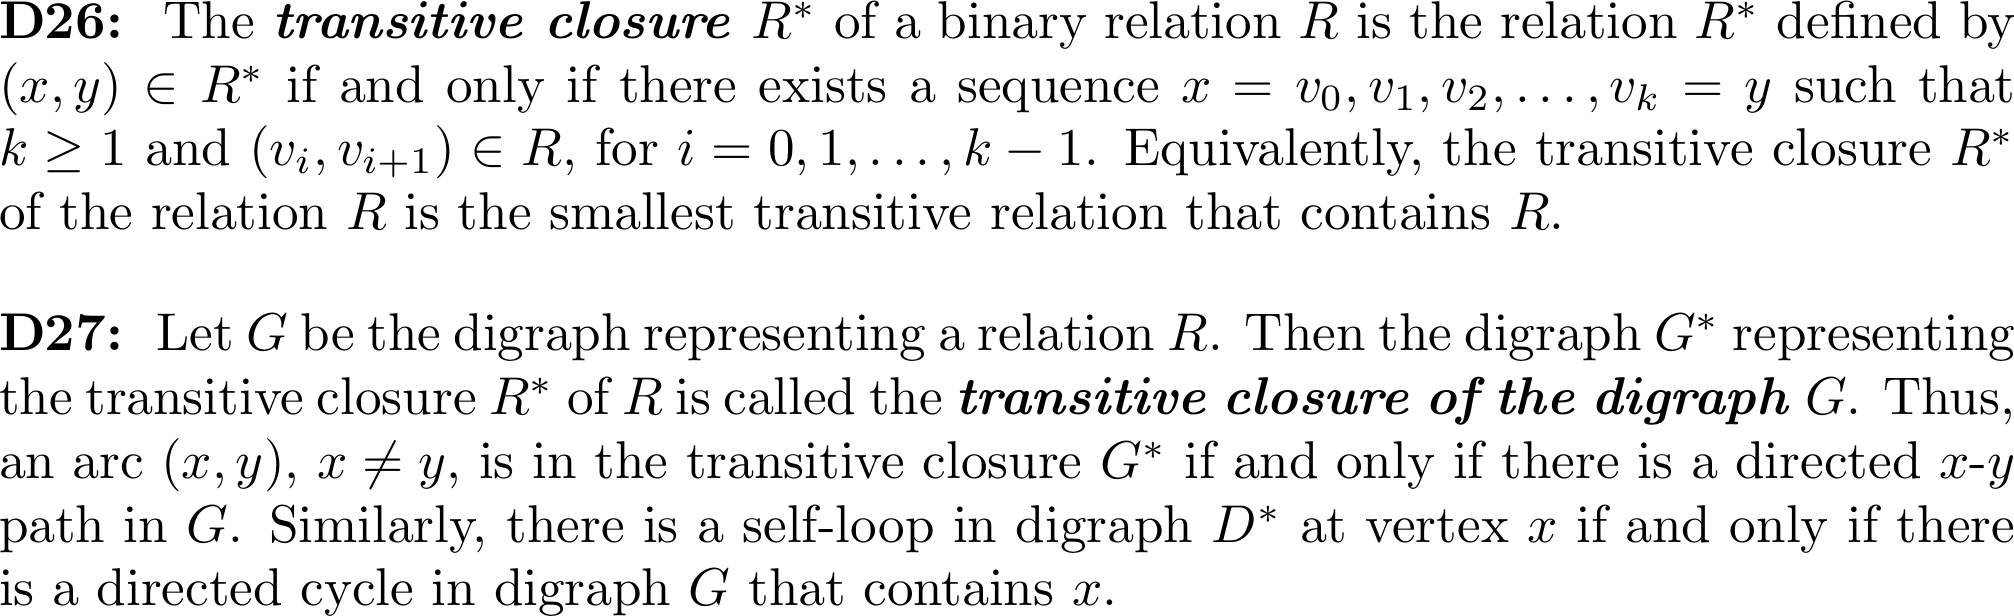
\includegraphics[width=.95\linewidth]{../img/grapht1.png}}
    \normalcolor%\caption{aus \cite[Seite 172]{gross2013handbook}}
\end{figure}

Oder kurz zusammengefasst: die transitive Hülle eines gerichteten Graphens $G$ ist wiederum ein gerichteter Graph $G^*$, der von jedem Knoten einen Bogen zu allen von diesem Knoten aus in $G$ erreichbaren Nachbarn besitzt. 

\newpage

In \cite[Seite 172]{gross2013handbook} ist hierzu folgendes Beispiel dargestellt:

\begin{figure}[H]
    \centering
    \setlength{\fboxsep}{10pt}\color{black!20}\fbox{
    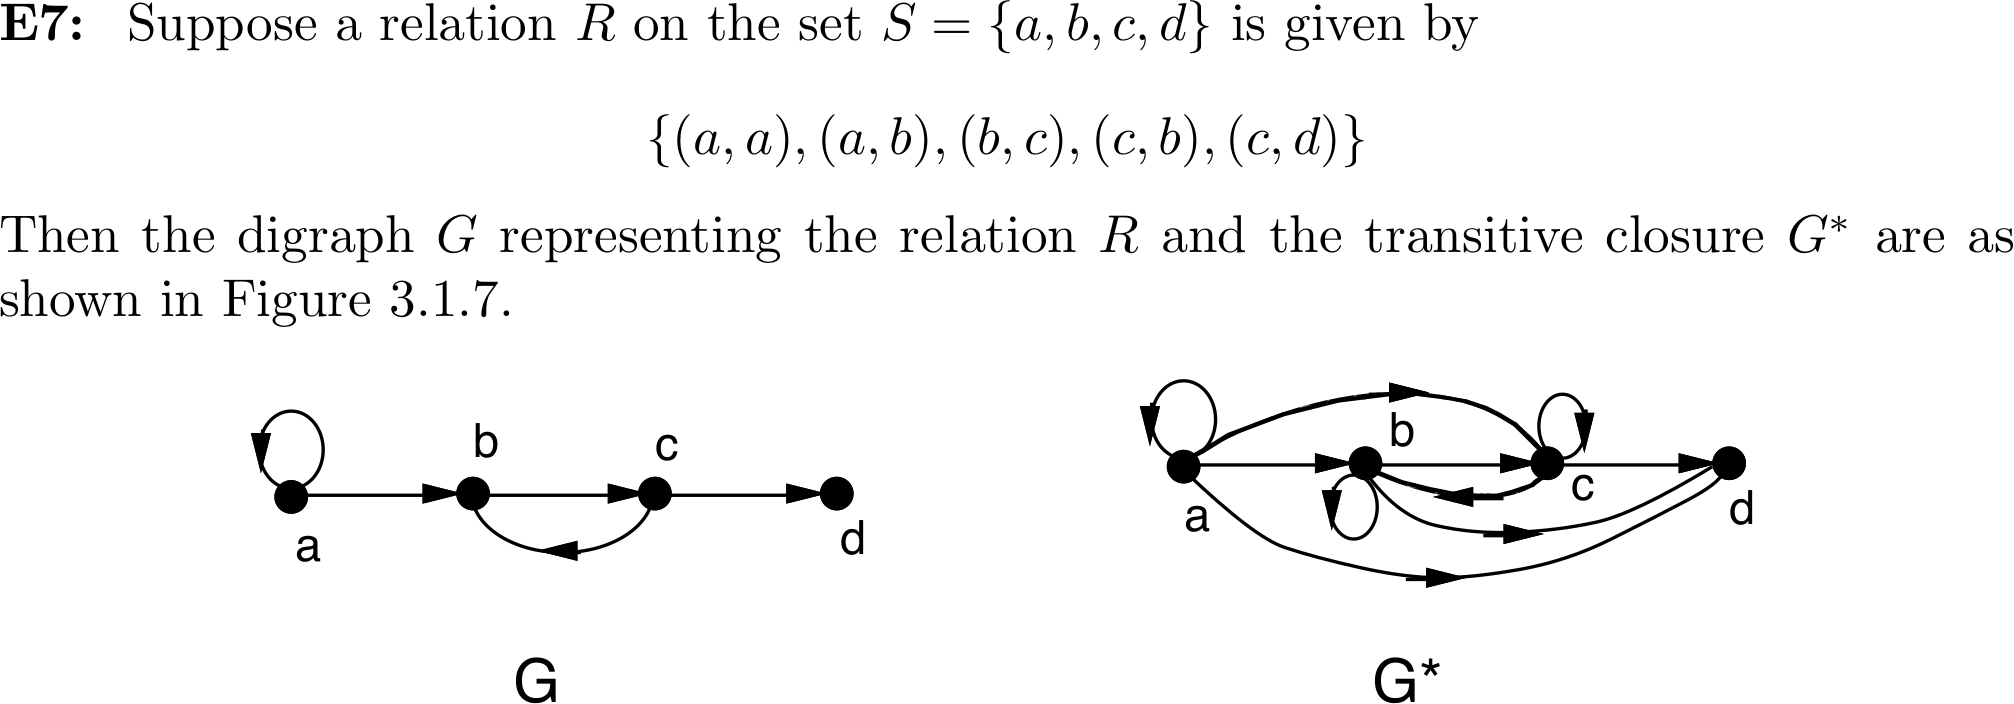
\includegraphics[width=.95\linewidth]{../img/grapht2.png}}
    \normalcolor%\caption{aus \cite[Seite 172]{gross2013handbook}}
\end{figure}

Es gibt mehrere Verfahren, um die transitive Hülle zu bestimmen. Es werden nun zwei Algorithmen vorgestellt, die anhand ihrer primären Suchrichtung benannt sind.

Wie in den Graphen dargestellt, läuft die \emph{horizontale} Suche primär über die Versionen -- mit jeweils einzelnen Kodes. Die \emph{vertikale} Suche läuft primär über die Kodes -- das heißt es werden zuerst alle Kodes einer Version gelesen.

\subsection{Horizontale Suche}

Ein intuitives Verfahren die transitive Hülle zu bestimmen wird in \cite[Seite 200]{jakobsson1991mixed} so beschrieben:

\begin{figure}[H]
    \centering
    \setlength{\fboxsep}{10pt}\color{black!20}\fbox{
    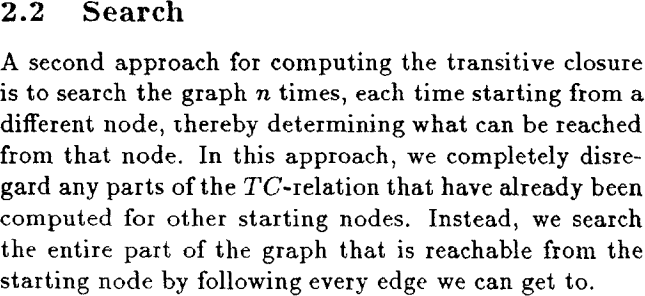
\includegraphics[width=.6\linewidth]{../img/search.png}}
    \normalcolor%\caption{aus \cite[Seite 200]{jakobsson1991mixed}}
    \vspace{-1em}
\end{figure}

Ähnlich wie im vorherigen Abschnitt für den Kode M21.6 dargestellt, werden also einfach ausgehend von einem Knoten so viele Suchen gestartet bis keine benachbarten Knoten mehr gefunden werden -- oder im Anwendungsfall der Umsteiger bis alle Versionen verarbeitet wurden.

Vorher erzielte Ergebnisse für andere Knoten, beziehungsweise Kodes, werden ignoriert. Das hieße im Beispiel oben, dass eine rückwärts chronologische Suche nach Umsteigern von M21.60 und M21.61 der ICD-10-GM Version ab dem Vorgänger M21.6 der Version 2014 zweimal exakt gleich ablaufen würde. 

Der Pseudocode für diese Vorgehensweise:

\begin{comment}
\begin{centernss}
\begin{struktogramm}(95,50)[test]
\assign{%
\begin{declaration}[Parameter:]
\description{\pVar{iPar}}{ an \pKey{int} parameter with the meaning described here}
\end{declaration}
\begin{declaration}[local Variables:]
\description{\pVar{iVar}}{an \pKey{int} variable with the meaning
described here}
\description{\pVar{dVar}}{a \pKey{double} variable with the
meaning described here}
\end{declaration}
}
\end{struktogramm}
\end{centernss}

\newpage
\end{comment}

%\subsection{SearchHorizontal}

\newpara{searchHorizontal}

Funktionsparameter:

\begin{comment}
\begin{itemize}
\item \texttt{system} \newline Das Kodiersystem, also zum Beispiel \texttt{icd10gm} oder \texttt{ops}. 
\item \texttt{version} \newline Version, beziehungsweise Jahrgang. 
\item \texttt{code} \newline Kode, nach dem gesucht wird. 
\end{itemize}
\end{comment}

\begin{itemize}
\item \texttt{\$system}, \texttt{\$version}, \texttt{\$code} \newline 
Wie Funktion readData, siehe Unterabschnitt \ref{function-read-data}.
\end{itemize}

Lokale Variable:

\begin{itemize}
\item \texttt{\$data} \hspace{2em} Rückgabewert, initial: leer.
\newline Eine assoziative Datenstruktur mit Key \texttt{fwd} $\Rightarrow$ Umsteiger, die chronologisch vorwärts von dem Suchkode erreichbar sind und \texttt{rev} $\Rightarrow$ chronologisch rückwärts. \\
\end{itemize}

\begin{comment}
\begingroup
\renewcommand{\arraystretch}{1.2}
\setlength{\tabcolsep}{12pt}
\begin{tabular}{|c|c|c|c|c|c|c|c|}
\hline
 & 2024 & 2023 & \dots & 2004 & 2.0 & 1.3 & \\
\hline
\end{tabular}
\endgroup
\end{comment}

\struktogrammAO{24}
{
\assign[\heightNS]{\$data[ 'fwd' ] = searchHorizontalRecursion (\$system, \$version, \$code, true)}
\assign[\heightNS]{\$data[ 'rev' ] = searchHorizontalRecursion (\$system, \$version, \$code, false)}
\return[\heightNS]{RETURN \$data}
}

\struktkommentar{Ausgehend von einem gegebenen Kodiersystem, Version, Kode wird chronologisch vorwärts und rückwärts eine rekursive Suche über alle Versionen gestartet.}

%\subsection{SearchHorizontalRecursion}

\newpara{searchHorizontalRecursion}

Funktionsparameter:

\begin{itemize}
\item \texttt{\$system}, \texttt{\$version}, \texttt{\$code} \newline Wie searchHorizontal. 
\item \texttt{\$chronological}
\newline Bestimmt die Suchrichtung. TRUE: chronologisch vorwärts und FALSE: rückwärts. 
\end{itemize}

Lokale Variablen:

\begin{itemize}
\item \texttt{\$data} \hspace{2em} Rückgabewert, initial: leer.
\newline Eine mehrdimensionale, assoziative Datenstruktur, die die Ergebnisse der rekursiven Suche enthält. Gefundene Umsteiger werden als Liste mit dem Key \texttt{umsteiger} gespeichert; zusätzlich zu den Listen wird auch die Versionen vorher und nachher notiert. Jeder einzelne Umsteiger-Eintrag enthält wiederum die Informationen zur automatischen Überleitbarkeit, sowie die Titel der Kodes vorher und nachher. Falls ein Umsteiger weitere Umsteiger hat, werden diese unter einem Key \texttt{recursion} abgelegt und die Suche fortgesetzt. Das heißt unter \texttt{recursion} ist das gleiche Datenkonstrukt nochmal enthalten. Ein Beispielergebnis für M21.6 befindet sich im Anhang \ref{search-horizontal-example}.
\item \texttt{\$otherVersion} \newline Die Version, zu der die Umsteiger ermittelt werden; \texttt{\$version} $\rightarrow$ \texttt{\$otherVersion}. 
\item \texttt{\$otherCode} \newline Die Spalte im Umsteiger-Eintrag, zu der der aktuelle Kode übergeleitet wird.
\item \texttt{\$readType} \newline Auf welche Art die Daten gelesen werden; siehe \texttt{readData}.
\item \texttt{\$umsteiger}, \texttt{\$entry} \newline Liste der Umsteiger, Schleifenvariable: Umsteiger-Eintrag.
\item \texttt{\$recursion} \newline Ergebnis des rekursiven Funktionsaufrufs bei gefundenen Umsteigern. \\
\end{itemize}

\struktogrammAO{35}{
    \ifthenelse[10]{1}{1}{IF \$chronological}{Y}{N}
        \assign[\heightNS]{\$otherVersion = \newline nextNewerVersion(\$system, \$version)}
        \assign[\heightNS]{\$readType = 'umsteiger\_join\_alt'}
        \assign[\heightNS]{\$otherCode = 'new'}
    \change
        \assign[\heightNS]{\$otherVersion = \newline nextOlderVersion(\$system, \$version)}
        \assign[\heightNS]{\$readType = 'umsteiger\_join'}
        \assign[\heightNS]{\$otherCode = 'old'}
    \ifend
}

\struktkommentar{Lokale Variablen werden anhand der Suchrichtung unterschiedlich belegt.}

\struktogrammAO{16}{
    \ifthenelse[10]{5}{1}{IF empty(\$version) OR empty(\$otherVersion)}{Y}{}
        \return[\heightNS]{RETURN \$data}
    \change
    \ifend
}

\struktkommentar{Falls es in der Suchrichtung keine weitere Version mehr gibt, endet die Rekursion.}

\struktogrammAO{27}{
    \assign[\heightNS]{\$umsteiger = readData(\$system, \$version, \$code, \$readType)}
    \ifthenelse[10]{5}{1}{IF empty(\$umsteiger)}{Y}{}
        \return[\heightNS]{RETURN \newline searchHorizontalRecursion(\$type, \$otherVersion, \$code, \$chronological)}
    \change
    \ifend
}

\struktkommentar{Die Umsteiger zwischen den Versionen im aktuellen Rekursionsschritt werden ermittelt. Falls es keine gibt --also keine, die eine Veränderung ausdrücken -- dann wird die Rekursion mit der nächsten Version fortgesetzt.}

%\texttt{readData ('icd10gm', '2014', 'M21.4', 'kodes')} 

\struktogrammAO{54}{
    \while[\heightNS]{FOREACH \$entry IN \$umsteiger}
        \ifthenelse[10]{5}{1}{IF \$entry[ \$otherCode ] IS NOT 'UNDEF'}{Y}{}
            \assign[\heightNS]{\$recursion = searchHorizontalRecursion \newline (\$system, \$version, \$entry[ \$otherCode ], \$chronological)}
            \ifthenelse[10]{4}{1}{IF NOT empty(\$recursion)}{Y}{}
                \assign[\heightNS]{\$entry[ 'recursion' ] = \$recursion}
            \change
            \ifend
        \change
        \ifend
        \assign[\heightNS]{\$data[ 'umsteiger' ][ ] = \$entry}
    \whileend
}

\struktkommentar{Für jeden Umsteiger wird die Rekursion mit dem veränderten Kode fortgesetzt. Allerdings nur falls dieser nicht UNDEF ist, weil es sich dann um einen entfernten oder neu hinzugefügten Kode handelt. Also wenn wie im Beispiel der M21.6 der ICD-10-GM Version 2013 die Umsteiger [ M21.60, M21.67, M21.87 ] in der Version 2012 hat, dann wird die Suche in die rückwärts chronologische Richtung mit diesen drei Kodes fortgesetzt statt mit M21.6. Die Ergebnisse dieser Verzweigung, sofern vorhanden, werden abgespeichert mit dem Key \texttt{recursion} zusätzlich zu jedem Umsteiger-Eintrag. Die Liste aller Umsteiger-Einträge, inklusive der UNDEF-Umsteiger, wird in das Ergebnis mit dem Key \texttt{umsteiger} aufgenommen.}

\struktogrammAO{23}{
    \assign[\heightNS]{\$data[ 'version' ] = \$version}
    \assign[\heightNS]{\$data[ 'other' ] = \$otherVersion}
    \return[\heightNS]{RETURN \$data}
}

\struktkommentar{Falls es Umsteiger für einen Kode gibt, werden zusätzlich die Versionen vorher und nachher gespeichert. Dann endet auch hier die Rekursion.}

Anhang \ref{search-horizontal-example} enthält das Ergebnis im JSON-Format für den Beispielaufruf der horizontale Suche für M21.6, Version 2014
%\texttt{searchHorizontal('icd10gm', '2014', 'M21.6')}
entsprechend der Abbildung \ref{img-m21-6}.

\begin{comment}
\struktogrammA{200}{searchUmsteigerHorizontal\_recursion
}{
    \assign[\heightNS]{ret = [ ]}
    \ifthenelse[10]{3}{1}{IF version === ' '}{TRUE}{FALSE}
        \return[\heightNS]{RETURN ret}
    \change
    \ifend
    \ifthenelse[10]{1}{1}{IF chronological}{TRUE}{FALSE}
        \assign[\heightNS]{other = nextNewerVersion(type, version)}
        \assign[\heightNS]{table = 'umsteiger\_join\_rev'}
        \assign[\heightNS]{which = 'new'}
    \change
        \assign[\heightNS]{other = nextOlderVersion(type, version)}
        \assign[\heightNS]{table = 'umsteiger\_join'}
        \assign[\heightNS]{which = 'old'}
    \ifend
    \ifthenelse[10]{3}{1}{IF other === ' '}{TRUE}{FALSE}
        \return[\heightNS]{RETURN ret}
    \change
    \ifend
    \assign[\heightNS]{umsteiger = readData(type, table, version, year, other, code)}
    \ifthenelse[10]{3}{1}{IF empty(umsteiger)}{TRUE}{FALSE}
        \return[\heightNS]{RETURN searchHorizontalRec(type, other, code, chronological)}
    \change
    \ifend
    \assign[\heightNS]{data = [ ]}
    \while[\heightNS]{FOREACH item IN umsteiger}
        \assign[\heightNS]{code = item[which]}
        \ifthenelse[10]{5}{1}{IF code !== 'UNDEF'}{TRUE}{FALSE}
            \assign[\heightNS]{recursion = searchHorizontalRec(type, other, search, chronological)}
            \ifthenelse[10]{4}{1}{IF NOT empty(recursion)}{TRUE}{FALSE}
                \assign[\heightNS]{item['recursion'] = recursion}
            \change
            \ifend
        \change
        \ifend
        \assign[\heightNS]{data[ ] = item}
    \whileend
    \assign[\heightNS]{ret['umsteiger'] = data}
    \assign[\heightNS]{ret['version'] = version}
    \assign[\heightNS]{ret['other'] = other}
    \return[\heightNS]{RETURN ret}
}
\end{comment}

\begin{comment}
{\small
\begin{struktogramm}(170,200)[searchUmsteigerHorizontal\_recursion]
    \assign[\heightNS]{ret = [ ]}
    \ifthenelse[10]{3}{1}{IF version === ' '}{TRUE}{FALSE}
        \return[\heightNS]{RETURN ret}
    \change
    \ifend
    \ifthenelse[10]{1}{1}{IF chronological}{TRUE}{FALSE}
        \assign[\heightNS]{other = nextNewerVersion(type, version)}
        \assign[\heightNS]{table = 'umsteiger\_join\_rev'}
        \assign[\heightNS]{which = 'new'}
    \change
        \assign[\heightNS]{other = nextOlderVersion(type, version)}
        \assign[\heightNS]{table = 'umsteiger\_join'}
        \assign[\heightNS]{which = 'old'}
    \ifend
    \ifthenelse[10]{3}{1}{IF other === ' '}{TRUE}{FALSE}
        \return[\heightNS]{RETURN ret}
    \change
    \ifend
    \assign[\heightNS]{umsteiger = readData(type, table, version, year, other, code)}
    \ifthenelse[10]{3}{1}{IF empty(umsteiger)}{TRUE}{FALSE}
        \return[\heightNS]{RETURN searchHorizontalRec(type, other, code, chronological)}
    \change
    \ifend
    \assign[\heightNS]{data = [ ]}
    \while[\heightNS]{FOREACH item IN umsteiger}
        \assign[\heightNS]{code = item[which]}
        \ifthenelse[10]{5}{1}{IF code !== 'UNDEF'}{TRUE}{FALSE}
            \assign[\heightNS]{recursion = searchHorizontalRec(type, other, search, chronological)}
            \ifthenelse[10]{4}{1}{IF NOT empty(recursion)}{TRUE}{FALSE}
                \assign[\heightNS]{item['recursion'] = recursion}
            \change
            \ifend
        \change
        \ifend
        \assign[\heightNS]{data[ ] = item}
    \whileend
    \assign[\heightNS]{ret['umsteiger'] = umsteiger}
    \assign[\heightNS]{ret['version'] = version}
    \assign[\heightNS]{ret['other'] = other}
    \return[\heightNS]{RETURN ret}
\end{struktogramm}
}
\end{comment}

% Bei UNDEF: array_unshift($umsteiger_out, $find);

\subsection{Vertikale Suche}
\label{vert-search}

Wie bereits erwähnt beginnt der Algorithmus der horizontalen Suche für jeden Kode ohne Vorkenntnisse über schon getätigte Aufrufe. Wenn die Umsteiger für alle Kodes einer Version --beziehungsweise eines ganzen Kodiersystems-- gefunden werden sollen, ist diese Vorgehensweise nicht effizient. 

Besonders für gerichtete Graphen ist allerdings Purdoms Algorithmus gut geeignet, um die transitive Hülle zu bestimmen, wie in \cite[Seite 77]{dar1993augmenting} beschrieben. Folgende kurze Zusammenfassung des Algorithmus basiert auf dieser Beschreibung, sowie auf \cite{purdom1970transitive} selbst: 

\begin{enumerate}
\item Ausgehend von einem Graphen $G$: Bestimme die stark zusammenhängenden Komponenten ($SCC$) in $G$ und vereinige diese in jeweils einen einzelnen Knoten. Das Ergebnis ist ein zyklenfreier, verdichteter Graph $G_c$.  %Let the original graph be G. Compute the strongly connected components in G, and collapse each one into a single node. Let the resulting acyclic condensation graph be Gc.
\item Sortiere $G_c$ topologisch. % Obtain a topological sort on Gc.
\item Ermittele die transitive Hülle von $G_c$ über dessen Adjazenzlisten in rückwärts topologischer Reihenfolge. % (Bestimme die erreichbaren Knoten über Adjazenzlisten) % Compute the transitive closure of Gc by expanding successor lists in reverse topological order.
\item Bestimme die transitive Hülle des ursprünglichen Graphens $G$ über die Nachbarschaftslisten der stark zusammenhängenen Komponenten in $G_c$: ein Knoten $y$ ist ein erreichbarer Nachbar von Knoten $x$, falls $SCC(y) = SCC(x)$ oder falls $SCC(y)$ ein erreichbarer Nachbar von $SCC(x)$ ist. % Compute the successor lists of the nodes in the original graph G from the successor lists of their respective SCCs: a node y is a successor of node x in G if SCC(y) = SCC(x) or SSC(y) is a succcessor of SCC(x) in Gc. 
\end{enumerate}

Die Vereinigung der stark zusammenhängenden Komponenten aus Schritt eins wird in \cite{purdom1970transitive} wie folgt dargestellt: 

%\begin{figure}[H]
%    \centering
%    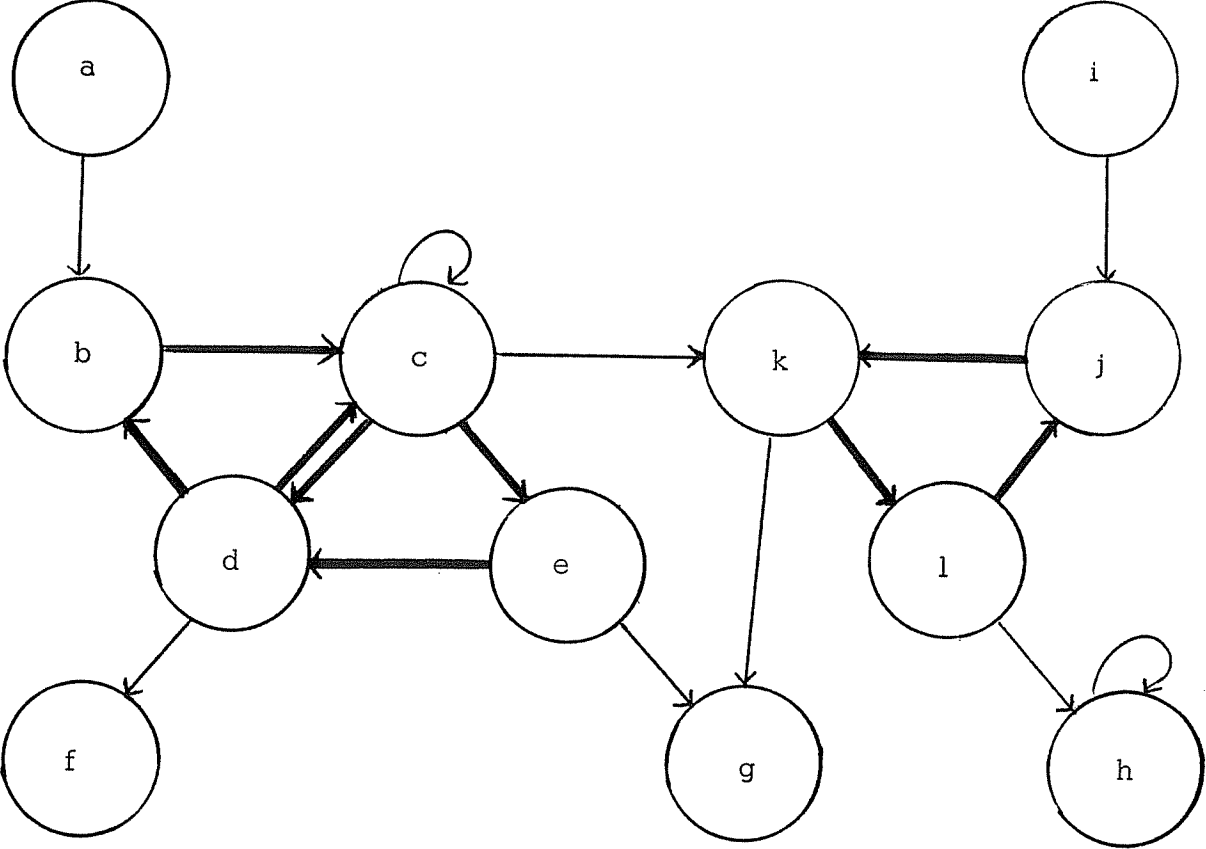
\includegraphics[width=.6\linewidth]{../img/purdom_g1.png}
%    \caption{Beispiel Graph $G$ von \cite[Seite 78]{purdom1970transitive}}
%\end{figure}

\begin{figure}[H]
    \centering
    \setlength{\fboxsep}{10pt}\color{black!20}\fbox{
    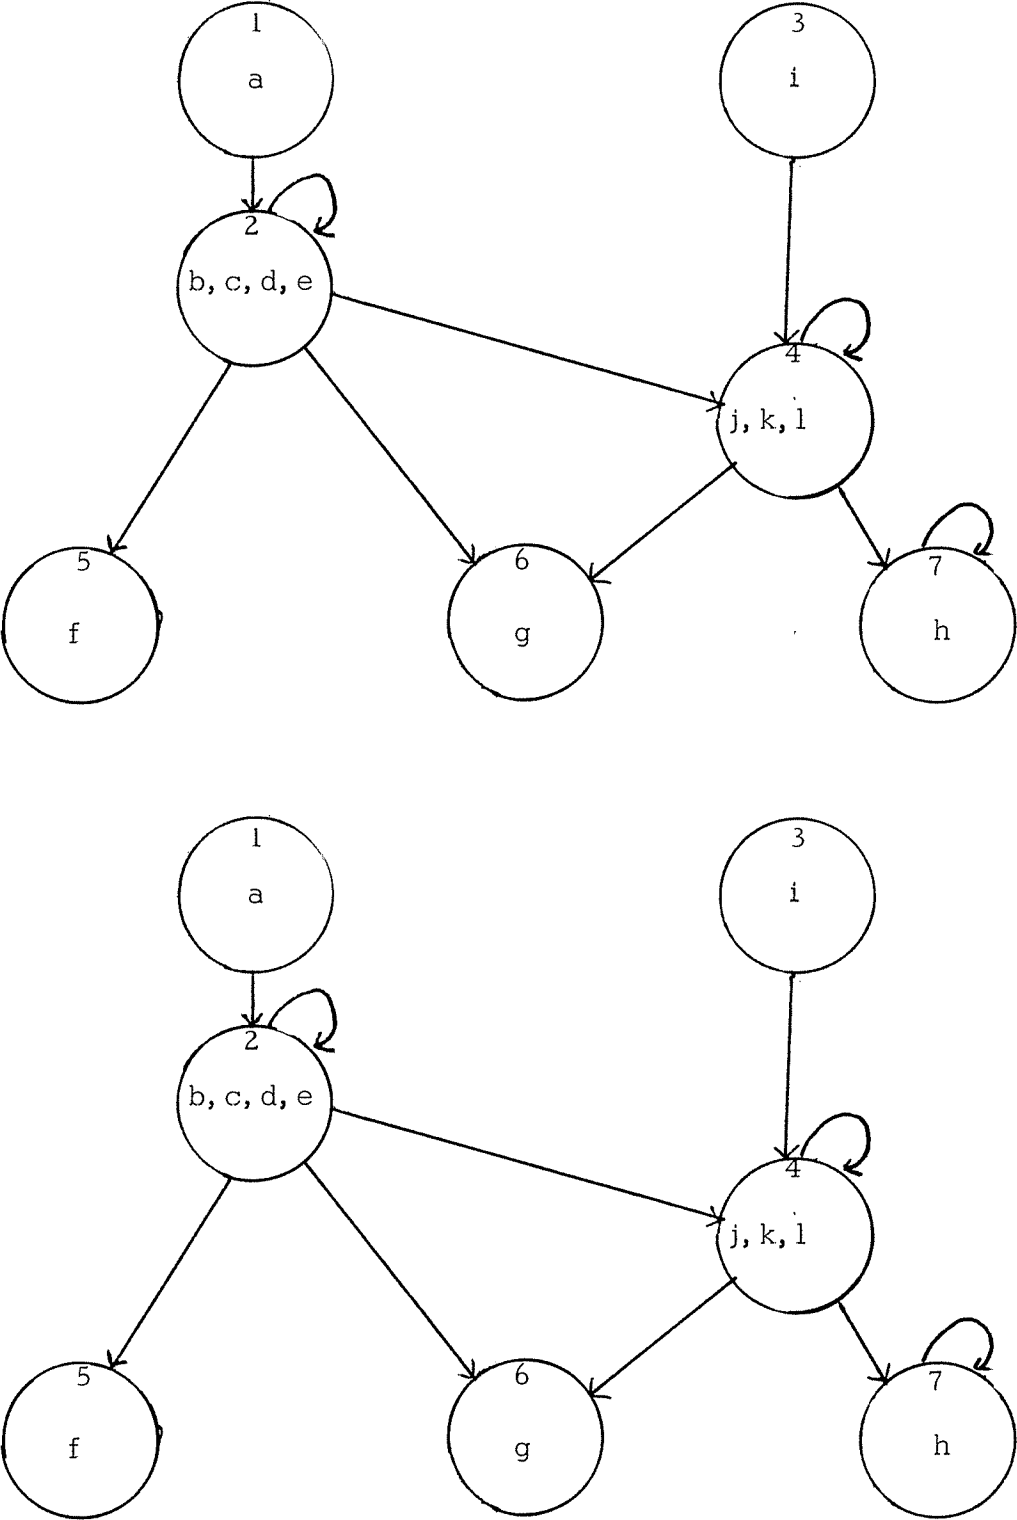
\includegraphics[width=.59\linewidth]{../img/purdom_g.png}}
    \normalcolor\caption{Beispielgraph $G$ und Vereinigung der stark zusammenhängenden Komponenten aus \cite[Seite 78]{purdom1970transitive}.}\vspace{-1.9em}
\end{figure}

Die hier vorgestellte vertikale Suche nach Umsteigern entspricht nicht ganz Purdoms Algorithmus. Sie weicht in mehreren Punkten ab:

\begin{itemize}
\item Die topologische Sortierung aus Schritt zwei in der Anwendung der Suche nach Umsteigern ist nicht notwendig, weil die Versionen immer in einer bestimmte Richtung verglichen werden und die Kodes sich nur zwischen zwei Versionen ändern können. Die Daten sind also schon implizit topologisch sortiert.
\item Ebenfalls ist nicht notwendig, die komplette transitiven Hülle zu ermitteln, sondern nur wie Kodes der Startversion in die Zielversion übergeleitet werden. Die Zwischenergebnisse werden trotzdem gespeichert. 
\item Auch bei der Suche nach Umsteigern nur mit Veränderungen ist es möglich, anders als bei den Knoten in einem Graphen, dass Kodes mehrmals vorkommen. Zum Beispiel gibt es G83.3 in ICD-10-GM nicht zwischen Version 2017 und 2005, aber schon davor und danach.  
\end{itemize} 

Trotzdem basiert die vertikale Suche wesentlich auf zwei Besonderheiten von Purdoms Algorithmus, die in \cite[Seite 76f]{dar1993augmenting} hervorgehoben werden:

\begin{figure}[H]
    \centering
    \setlength{\fboxsep}{10pt}\color{black!20}\fbox{
    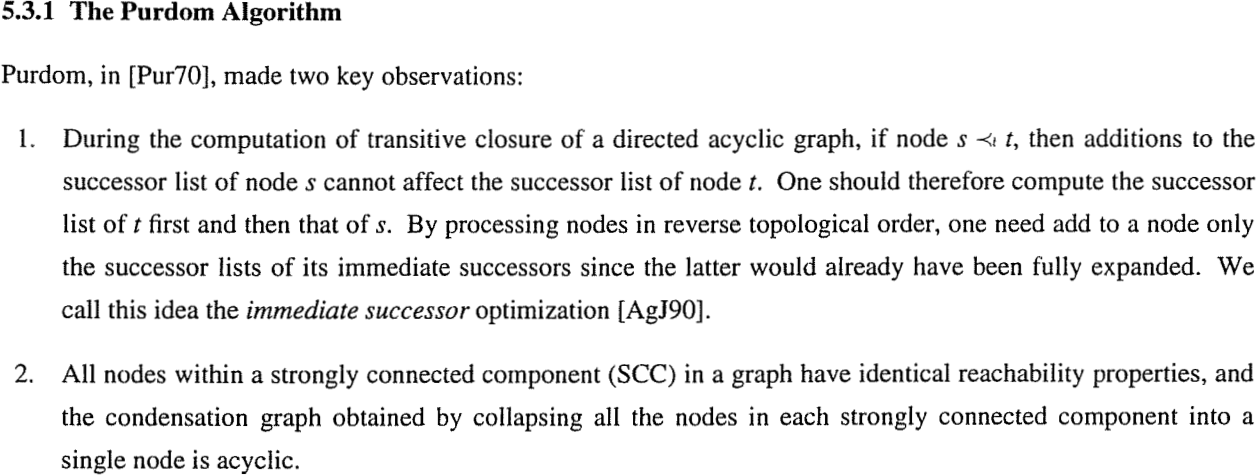
\includegraphics[width=.99\linewidth]{../img/purdom_r.png}}
    \normalcolor%\caption{aus \cite[Seite 76f]{dar1993augmenting}}
\end{figure}

Konkret bedeuten diese Besonderheiten für die Umsteiger-Suche:

\begin{enumerate}
\item Topologisch rückwärts gerichtete Vorgehensweise:\newline So ist zum Beispiel bei der Suche nach den Umsteigern eines ICD-GM-10 Kodes der Version 1.3 die Reihenfolge, in der die anderen Versionen abgearbeitet werden: 2024, 2023, 2022 und so weiter. Oder anders ausgedrückt: Wenn die Überleitungen in chronologischer Reihenfolge bestimmt werden sollen, dann läuft die vertikale Suche umgekehrt, also chronologisch rückwärts. 
\item Vereinigung der stark zusammenhängenden Komponenten:\newline Nach jedem Schritt über eine Version, wird geprüft, ob ein neu gefundener Umsteiger eine Überleitung in einen Kode enthält, der bereits in den davor abgearbeiteten Versionen als Umsteiger vorkommt. Falls ja, dann werden diese Umsteiger vereinigt, das heißt die Zwischenschritte werden zu einem Schritt zusammengefügt. 
\end{enumerate}

\ \\

Abbildung \ref{merge-illustrated} auf der nächsten Seite zeigt ein einfaches Beispiel für die Vereinigung: 

Angenommen ein abstraktes System hat Umsteiger von der Version 1.0 auf 2.0: $A$$\rightarrow$$B$ und $M$$\rightarrow$$N$, sowie von Version 2.0 auf 3.0: $B$$\rightarrow$$C$. Wenn nun in chronologischer Reihenfolge 1.0$\rightarrow$2.0$\rightarrow$3.0 Umsteiger ermittelt werden sollen, erfolgt die Suche sowie Vereinigung gefundener Umsteiger in umgekehrter Reihenfolge. Das heißt wenn im Schritt 3.0$\leftarrow$2.0 der Umsteiger $C$$\leftarrow$$B$ gefunden wird, dann wird danach bei der Vereinigung mit Version 1.0 der Umsteiger $B$$\leftarrow$$A$ in $C$$\leftarrow$$A$ umgewandelt. $A$ in Version 1.0 entspricht $C$ in Version 3.0. 

Falls es Verzweigungen gibt, also es mehrere Umsteiger für einen Kode gibt, dann werden entsprechend Listen vereinigt. Ein reales Beispiel dazu folgt später. 

\begin{figure}[H]
    \centering\Huge%\sffamily
    \resizebox{.75\linewidth}{!}{% Graphic for TeX using PGF
% Title: /home/simon/jacuke_ma/tex/dia/merge.dia
% Creator: Dia v0.97+git
% CreationDate: Mon Oct 28 09:00:01 2024
% For: simon
% \usepackage{tikz}
% The following commands are not supported in PSTricks at present
% We define them conditionally, so when they are implemented,
% this pgf file will use them.
\ifx\du\undefined
  \newlength{\du}
\fi
\setlength{\du}{15\unitlength}
\begin{tikzpicture}[even odd rule]
\pgftransformxscale{1.000000}
\pgftransformyscale{-1.000000}
\definecolor{dialinecolor}{rgb}{0.000000, 0.000000, 0.000000}
\pgfsetstrokecolor{dialinecolor}
\pgfsetstrokeopacity{1.000000}
\definecolor{diafillcolor}{rgb}{1.000000, 1.000000, 1.000000}
\pgfsetfillcolor{diafillcolor}
\pgfsetfillopacity{1.000000}
\pgfsetlinewidth{0.100000\du}
\pgfsetdash{}{0pt}
\pgfsetmiterjoin
\pgfsetbuttcap
{\pgfsetcornersarced{\pgfpoint{0.000000\du}{0.000000\du}}\definecolor{diafillcolor}{rgb}{1.000000, 1.000000, 1.000000}
\pgfsetfillcolor{diafillcolor}
\pgfsetfillopacity{0.117647}
\fill (-26.000000\du,-33.000000\du)--(-26.000000\du,-6.000000\du)--(29.000000\du,-6.000000\du)--(29.000000\du,-33.000000\du)--cycle;
}{\pgfsetcornersarced{\pgfpoint{0.000000\du}{0.000000\du}}\definecolor{dialinecolor}{rgb}{1.000000, 1.000000, 1.000000}
\pgfsetstrokecolor{dialinecolor}
\pgfsetstrokeopacity{1.000000}
\draw (-26.000000\du,-33.000000\du)--(-26.000000\du,-6.000000\du)--(29.000000\du,-6.000000\du)--(29.000000\du,-33.000000\du)--cycle;
}\pgfsetlinewidth{0.100000\du}
\pgfsetdash{}{0pt}
\pgfsetroundjoin
\pgfsetbuttcap
{\pgfsetcornersarced{\pgfpoint{2.000000\du}{2.000000\du}}\definecolor{diafillcolor}{rgb}{1.000000, 1.000000, 1.000000}
\pgfsetfillcolor{diafillcolor}
\pgfsetfillopacity{1.000000}
\fill (-9.000000\du,-27.000000\du)--(-9.000000\du,-7.000000\du)--(5.000000\du,-7.000000\du)--(5.000000\du,-27.000000\du)--cycle;
}{\pgfsetcornersarced{\pgfpoint{2.000000\du}{2.000000\du}}\definecolor{dialinecolor}{rgb}{0.411765, 0.411765, 0.411765}
\pgfsetstrokecolor{dialinecolor}
\pgfsetstrokeopacity{1.000000}
\draw (-9.000000\du,-27.000000\du)--(-9.000000\du,-7.000000\du)--(5.000000\du,-7.000000\du)--(5.000000\du,-27.000000\du)--cycle;
}\pgfsetlinewidth{0.100000\du}
\pgfsetdash{}{0pt}
\pgfsetroundjoin
\pgfsetbuttcap
{\pgfsetcornersarced{\pgfpoint{2.000000\du}{2.000000\du}}\definecolor{diafillcolor}{rgb}{1.000000, 1.000000, 1.000000}
\pgfsetfillcolor{diafillcolor}
\pgfsetfillopacity{1.000000}
\fill (-25.000000\du,-27.000000\du)--(-25.000000\du,-7.000000\du)--(-11.000000\du,-7.000000\du)--(-11.000000\du,-27.000000\du)--cycle;
}{\pgfsetcornersarced{\pgfpoint{2.000000\du}{2.000000\du}}\definecolor{dialinecolor}{rgb}{0.411765, 0.411765, 0.411765}
\pgfsetstrokecolor{dialinecolor}
\pgfsetstrokeopacity{1.000000}
\draw (-25.000000\du,-27.000000\du)--(-25.000000\du,-7.000000\du)--(-11.000000\du,-7.000000\du)--(-11.000000\du,-27.000000\du)--cycle;
}\pgfsetlinewidth{0.100000\du}
\pgfsetdash{}{0pt}
\definecolor{diafillcolor}{rgb}{1.000000, 1.000000, 1.000000}
\pgfsetfillcolor{diafillcolor}
\pgfsetfillopacity{1.000000}
\pgfpathellipse{\pgfpoint{-15.000000\du}{-23.000000\du}}{\pgfpoint{2.000000\du}{0\du}}{\pgfpoint{0\du}{2.000000\du}}
\pgfusepath{fill}
\definecolor{dialinecolor}{rgb}{0.000000, 0.000000, 0.000000}
\pgfsetstrokecolor{dialinecolor}
\pgfsetstrokeopacity{1.000000}
\pgfpathellipse{\pgfpoint{-15.000000\du}{-23.000000\du}}{\pgfpoint{2.000000\du}{0\du}}{\pgfpoint{0\du}{2.000000\du}}
\pgfusepath{stroke}
% setfont left to latex
\definecolor{dialinecolor}{rgb}{0.000000, 0.000000, 0.000000}
\pgfsetstrokecolor{dialinecolor}
\pgfsetstrokeopacity{1.000000}
\definecolor{diafillcolor}{rgb}{0.000000, 0.000000, 0.000000}
\pgfsetfillcolor{diafillcolor}
\pgfsetfillopacity{1.000000}
\node[anchor=base,inner sep=0pt, outer sep=0pt,color=dialinecolor] at (-15.000000\du,-22.354276\du){B};
\pgfsetlinewidth{0.200000\du}
\pgfsetdash{}{0pt}
\pgfsetbuttcap
{
\definecolor{diafillcolor}{rgb}{0.000000, 0.000000, 0.000000}
\pgfsetfillcolor{diafillcolor}
\pgfsetfillopacity{1.000000}
% was here!!!
\pgfsetarrowsend{stealth}
\definecolor{dialinecolor}{rgb}{0.000000, 0.000000, 0.000000}
\pgfsetstrokecolor{dialinecolor}
\pgfsetstrokeopacity{1.000000}
\draw (-17.044922\du,-23.000000\du)--(-18.955078\du,-23.000000\du);
}
\pgfsetlinewidth{0.100000\du}
\pgfsetdash{}{0pt}
\definecolor{diafillcolor}{rgb}{1.000000, 1.000000, 1.000000}
\pgfsetfillcolor{diafillcolor}
\pgfsetfillopacity{1.000000}
\pgfpathellipse{\pgfpoint{-21.000000\du}{-23.000000\du}}{\pgfpoint{2.000000\du}{0\du}}{\pgfpoint{0\du}{2.000000\du}}
\pgfusepath{fill}
\definecolor{dialinecolor}{rgb}{0.000000, 0.000000, 0.000000}
\pgfsetstrokecolor{dialinecolor}
\pgfsetstrokeopacity{1.000000}
\pgfpathellipse{\pgfpoint{-21.000000\du}{-23.000000\du}}{\pgfpoint{2.000000\du}{0\du}}{\pgfpoint{0\du}{2.000000\du}}
\pgfusepath{stroke}
% setfont left to latex
\definecolor{dialinecolor}{rgb}{0.000000, 0.000000, 0.000000}
\pgfsetstrokecolor{dialinecolor}
\pgfsetstrokeopacity{1.000000}
\definecolor{diafillcolor}{rgb}{0.000000, 0.000000, 0.000000}
\pgfsetfillcolor{diafillcolor}
\pgfsetfillopacity{1.000000}
\node[anchor=base,inner sep=0pt, outer sep=0pt,color=dialinecolor] at (-21.000000\du,-22.354276\du){C};
\pgfsetlinewidth{0.100000\du}
\pgfsetdash{}{0pt}
\definecolor{diafillcolor}{rgb}{1.000000, 1.000000, 1.000000}
\pgfsetfillcolor{diafillcolor}
\pgfsetfillopacity{1.000000}
\pgfpathellipse{\pgfpoint{1.000000\du}{-17.000000\du}}{\pgfpoint{2.000000\du}{0\du}}{\pgfpoint{0\du}{2.000000\du}}
\pgfusepath{fill}
\definecolor{dialinecolor}{rgb}{0.000000, 0.000000, 0.000000}
\pgfsetstrokecolor{dialinecolor}
\pgfsetstrokeopacity{1.000000}
\pgfpathellipse{\pgfpoint{1.000000\du}{-17.000000\du}}{\pgfpoint{2.000000\du}{0\du}}{\pgfpoint{0\du}{2.000000\du}}
\pgfusepath{stroke}
% setfont left to latex
\definecolor{dialinecolor}{rgb}{0.000000, 0.000000, 0.000000}
\pgfsetstrokecolor{dialinecolor}
\pgfsetstrokeopacity{1.000000}
\definecolor{diafillcolor}{rgb}{0.000000, 0.000000, 0.000000}
\pgfsetfillcolor{diafillcolor}
\pgfsetfillopacity{1.000000}
\node[anchor=base,inner sep=0pt, outer sep=0pt,color=dialinecolor] at (1.000000\du,-16.354276\du){A};
\pgfsetlinewidth{0.200000\du}
\pgfsetdash{}{0pt}
\pgfsetbuttcap
{
\definecolor{diafillcolor}{rgb}{0.000000, 0.000000, 0.000000}
\pgfsetfillcolor{diafillcolor}
\pgfsetfillopacity{1.000000}
% was here!!!
\pgfsetarrowsend{stealth}
\definecolor{dialinecolor}{rgb}{0.000000, 0.000000, 0.000000}
\pgfsetstrokecolor{dialinecolor}
\pgfsetstrokeopacity{1.000000}
\draw (-1.044922\du,-17.000000\du)--(-2.955078\du,-17.000000\du);
}
\pgfsetlinewidth{0.100000\du}
\pgfsetdash{}{0pt}
\definecolor{diafillcolor}{rgb}{1.000000, 1.000000, 1.000000}
\pgfsetfillcolor{diafillcolor}
\pgfsetfillopacity{1.000000}
\pgfpathellipse{\pgfpoint{-5.000000\du}{-17.000000\du}}{\pgfpoint{2.000000\du}{0\du}}{\pgfpoint{0\du}{2.000000\du}}
\pgfusepath{fill}
\definecolor{dialinecolor}{rgb}{0.000000, 0.000000, 0.000000}
\pgfsetstrokecolor{dialinecolor}
\pgfsetstrokeopacity{1.000000}
\pgfpathellipse{\pgfpoint{-5.000000\du}{-17.000000\du}}{\pgfpoint{2.000000\du}{0\du}}{\pgfpoint{0\du}{2.000000\du}}
\pgfusepath{stroke}
% setfont left to latex
\definecolor{dialinecolor}{rgb}{0.000000, 0.000000, 0.000000}
\pgfsetstrokecolor{dialinecolor}
\pgfsetstrokeopacity{1.000000}
\definecolor{diafillcolor}{rgb}{0.000000, 0.000000, 0.000000}
\pgfsetfillcolor{diafillcolor}
\pgfsetfillopacity{1.000000}
\node[anchor=base,inner sep=0pt, outer sep=0pt,color=dialinecolor] at (-5.000000\du,-16.354276\du){B};
\pgfsetlinewidth{0.100000\du}
\pgfsetdash{}{0pt}
\definecolor{diafillcolor}{rgb}{1.000000, 1.000000, 1.000000}
\pgfsetfillcolor{diafillcolor}
\pgfsetfillopacity{1.000000}
\pgfpathellipse{\pgfpoint{1.000000\du}{-11.000000\du}}{\pgfpoint{2.000000\du}{0\du}}{\pgfpoint{0\du}{2.000000\du}}
\pgfusepath{fill}
\definecolor{dialinecolor}{rgb}{0.000000, 0.000000, 0.000000}
\pgfsetstrokecolor{dialinecolor}
\pgfsetstrokeopacity{1.000000}
\pgfpathellipse{\pgfpoint{1.000000\du}{-11.000000\du}}{\pgfpoint{2.000000\du}{0\du}}{\pgfpoint{0\du}{2.000000\du}}
\pgfusepath{stroke}
% setfont left to latex
\definecolor{dialinecolor}{rgb}{0.000000, 0.000000, 0.000000}
\pgfsetstrokecolor{dialinecolor}
\pgfsetstrokeopacity{1.000000}
\definecolor{diafillcolor}{rgb}{0.000000, 0.000000, 0.000000}
\pgfsetfillcolor{diafillcolor}
\pgfsetfillopacity{1.000000}
\node[anchor=base,inner sep=0pt, outer sep=0pt,color=dialinecolor] at (1.000000\du,-10.354276\du){M};
\pgfsetlinewidth{0.200000\du}
\pgfsetdash{}{0pt}
\pgfsetbuttcap
{
\definecolor{diafillcolor}{rgb}{0.000000, 0.000000, 0.000000}
\pgfsetfillcolor{diafillcolor}
\pgfsetfillopacity{1.000000}
% was here!!!
\pgfsetarrowsend{stealth}
\definecolor{dialinecolor}{rgb}{0.000000, 0.000000, 0.000000}
\pgfsetstrokecolor{dialinecolor}
\pgfsetstrokeopacity{1.000000}
\draw (-1.044922\du,-11.000000\du)--(-2.955078\du,-11.000000\du);
}
\pgfsetlinewidth{0.100000\du}
\pgfsetdash{}{0pt}
\definecolor{diafillcolor}{rgb}{1.000000, 1.000000, 1.000000}
\pgfsetfillcolor{diafillcolor}
\pgfsetfillopacity{1.000000}
\pgfpathellipse{\pgfpoint{-5.000000\du}{-11.000000\du}}{\pgfpoint{2.000000\du}{0\du}}{\pgfpoint{0\du}{2.000000\du}}
\pgfusepath{fill}
\definecolor{dialinecolor}{rgb}{0.000000, 0.000000, 0.000000}
\pgfsetstrokecolor{dialinecolor}
\pgfsetstrokeopacity{1.000000}
\pgfpathellipse{\pgfpoint{-5.000000\du}{-11.000000\du}}{\pgfpoint{2.000000\du}{0\du}}{\pgfpoint{0\du}{2.000000\du}}
\pgfusepath{stroke}
% setfont left to latex
\definecolor{dialinecolor}{rgb}{0.000000, 0.000000, 0.000000}
\pgfsetstrokecolor{dialinecolor}
\pgfsetstrokeopacity{1.000000}
\definecolor{diafillcolor}{rgb}{0.000000, 0.000000, 0.000000}
\pgfsetfillcolor{diafillcolor}
\pgfsetfillopacity{1.000000}
\node[anchor=base,inner sep=0pt, outer sep=0pt,color=dialinecolor] at (-5.000000\du,-10.354276\du){N};
\pgfsetlinewidth{0.100000\du}
\pgfsetdash{}{0pt}
\pgfsetroundjoin
\pgfsetbuttcap
{\pgfsetcornersarced{\pgfpoint{2.000000\du}{2.000000\du}}\definecolor{diafillcolor}{rgb}{1.000000, 1.000000, 1.000000}
\pgfsetfillcolor{diafillcolor}
\pgfsetfillopacity{1.000000}
\fill (-22.000000\du,-32.000000\du)--(-22.000000\du,-28.000000\du)--(-14.000000\du,-28.000000\du)--(-14.000000\du,-32.000000\du)--cycle;
}{\pgfsetcornersarced{\pgfpoint{2.000000\du}{2.000000\du}}\definecolor{dialinecolor}{rgb}{0.411765, 0.411765, 0.411765}
\pgfsetstrokecolor{dialinecolor}
\pgfsetstrokeopacity{1.000000}
\draw (-22.000000\du,-32.000000\du)--(-22.000000\du,-28.000000\du)--(-14.000000\du,-28.000000\du)--(-14.000000\du,-32.000000\du)--cycle;
}% setfont left to latex
\definecolor{dialinecolor}{rgb}{0.000000, 0.000000, 0.000000}
\pgfsetstrokecolor{dialinecolor}
\pgfsetstrokeopacity{1.000000}
\definecolor{diafillcolor}{rgb}{0.000000, 0.000000, 0.000000}
\pgfsetfillcolor{diafillcolor}
\pgfsetfillopacity{1.000000}
\node[anchor=base,inner sep=0pt, outer sep=0pt,color=dialinecolor] at (-18.000000\du,-29.381708\du){3.0 – 2.0};
\pgfsetlinewidth{0.100000\du}
\pgfsetdash{}{0pt}
\pgfsetroundjoin
\pgfsetbuttcap
{\pgfsetcornersarced{\pgfpoint{2.000000\du}{2.000000\du}}\definecolor{diafillcolor}{rgb}{1.000000, 1.000000, 1.000000}
\pgfsetfillcolor{diafillcolor}
\pgfsetfillopacity{1.000000}
\fill (-6.000000\du,-32.000000\du)--(-6.000000\du,-28.000000\du)--(2.000000\du,-28.000000\du)--(2.000000\du,-32.000000\du)--cycle;
}{\pgfsetcornersarced{\pgfpoint{2.000000\du}{2.000000\du}}\definecolor{dialinecolor}{rgb}{0.411765, 0.411765, 0.411765}
\pgfsetstrokecolor{dialinecolor}
\pgfsetstrokeopacity{1.000000}
\draw (-6.000000\du,-32.000000\du)--(-6.000000\du,-28.000000\du)--(2.000000\du,-28.000000\du)--(2.000000\du,-32.000000\du)--cycle;
}% setfont left to latex
\definecolor{dialinecolor}{rgb}{0.000000, 0.000000, 0.000000}
\pgfsetstrokecolor{dialinecolor}
\pgfsetstrokeopacity{1.000000}
\definecolor{diafillcolor}{rgb}{0.000000, 0.000000, 0.000000}
\pgfsetfillcolor{diafillcolor}
\pgfsetfillopacity{1.000000}
\node[anchor=base,inner sep=0pt, outer sep=0pt,color=dialinecolor] at (-2.000000\du,-29.381708\du){2.0 – 1.0};
\pgfsetlinewidth{0.100000\du}
\pgfsetdash{}{0pt}
\pgfsetroundjoin
\pgfsetbuttcap
{\pgfsetcornersarced{\pgfpoint{2.000000\du}{2.000000\du}}\definecolor{diafillcolor}{rgb}{1.000000, 1.000000, 1.000000}
\pgfsetfillcolor{diafillcolor}
\pgfsetfillopacity{1.000000}
\fill (14.000000\du,-27.000000\du)--(14.000000\du,-7.000000\du)--(28.000000\du,-7.000000\du)--(28.000000\du,-27.000000\du)--cycle;
}{\pgfsetcornersarced{\pgfpoint{2.000000\du}{2.000000\du}}\definecolor{dialinecolor}{rgb}{0.411765, 0.411765, 0.411765}
\pgfsetstrokecolor{dialinecolor}
\pgfsetstrokeopacity{1.000000}
\draw (14.000000\du,-27.000000\du)--(14.000000\du,-7.000000\du)--(28.000000\du,-7.000000\du)--(28.000000\du,-27.000000\du)--cycle;
}\pgfsetlinewidth{0.100000\du}
\pgfsetdash{}{0pt}
\definecolor{diafillcolor}{rgb}{1.000000, 1.000000, 1.000000}
\pgfsetfillcolor{diafillcolor}
\pgfsetfillopacity{1.000000}
\pgfpathellipse{\pgfpoint{24.000000\du}{-17.000000\du}}{\pgfpoint{2.000000\du}{0\du}}{\pgfpoint{0\du}{2.000000\du}}
\pgfusepath{fill}
\definecolor{dialinecolor}{rgb}{0.000000, 0.000000, 0.000000}
\pgfsetstrokecolor{dialinecolor}
\pgfsetstrokeopacity{1.000000}
\pgfpathellipse{\pgfpoint{24.000000\du}{-17.000000\du}}{\pgfpoint{2.000000\du}{0\du}}{\pgfpoint{0\du}{2.000000\du}}
\pgfusepath{stroke}
% setfont left to latex
\definecolor{dialinecolor}{rgb}{0.000000, 0.000000, 0.000000}
\pgfsetstrokecolor{dialinecolor}
\pgfsetstrokeopacity{1.000000}
\definecolor{diafillcolor}{rgb}{0.000000, 0.000000, 0.000000}
\pgfsetfillcolor{diafillcolor}
\pgfsetfillopacity{1.000000}
\node[anchor=base,inner sep=0pt, outer sep=0pt,color=dialinecolor] at (24.000000\du,-16.354276\du){A};
\pgfsetlinewidth{0.200000\du}
\pgfsetdash{}{0pt}
\pgfsetbuttcap
{
\definecolor{diafillcolor}{rgb}{0.000000, 0.000000, 0.000000}
\pgfsetfillcolor{diafillcolor}
\pgfsetfillopacity{1.000000}
% was here!!!
\pgfsetarrowsend{stealth}
\definecolor{dialinecolor}{rgb}{0.000000, 0.000000, 0.000000}
\pgfsetstrokecolor{dialinecolor}
\pgfsetstrokeopacity{1.000000}
\draw (21.955078\du,-17.000000\du)--(20.044922\du,-17.000000\du);
}
\pgfsetlinewidth{0.100000\du}
\pgfsetdash{}{0pt}
\definecolor{diafillcolor}{rgb}{1.000000, 1.000000, 1.000000}
\pgfsetfillcolor{diafillcolor}
\pgfsetfillopacity{1.000000}
\pgfpathellipse{\pgfpoint{18.000000\du}{-17.000000\du}}{\pgfpoint{2.000000\du}{0\du}}{\pgfpoint{0\du}{2.000000\du}}
\pgfusepath{fill}
\definecolor{dialinecolor}{rgb}{0.000000, 0.000000, 0.000000}
\pgfsetstrokecolor{dialinecolor}
\pgfsetstrokeopacity{1.000000}
\pgfpathellipse{\pgfpoint{18.000000\du}{-17.000000\du}}{\pgfpoint{2.000000\du}{0\du}}{\pgfpoint{0\du}{2.000000\du}}
\pgfusepath{stroke}
% setfont left to latex
\definecolor{dialinecolor}{rgb}{0.000000, 0.000000, 0.000000}
\pgfsetstrokecolor{dialinecolor}
\pgfsetstrokeopacity{1.000000}
\definecolor{diafillcolor}{rgb}{0.000000, 0.000000, 0.000000}
\pgfsetfillcolor{diafillcolor}
\pgfsetfillopacity{1.000000}
\node[anchor=base,inner sep=0pt, outer sep=0pt,color=dialinecolor] at (18.000000\du,-16.354276\du){C};
\pgfsetlinewidth{0.100000\du}
\pgfsetdash{}{0pt}
\definecolor{diafillcolor}{rgb}{1.000000, 1.000000, 1.000000}
\pgfsetfillcolor{diafillcolor}
\pgfsetfillopacity{1.000000}
\pgfpathellipse{\pgfpoint{24.000000\du}{-23.000000\du}}{\pgfpoint{2.000000\du}{0\du}}{\pgfpoint{0\du}{2.000000\du}}
\pgfusepath{fill}
\definecolor{dialinecolor}{rgb}{0.000000, 0.000000, 0.000000}
\pgfsetstrokecolor{dialinecolor}
\pgfsetstrokeopacity{1.000000}
\pgfpathellipse{\pgfpoint{24.000000\du}{-23.000000\du}}{\pgfpoint{2.000000\du}{0\du}}{\pgfpoint{0\du}{2.000000\du}}
\pgfusepath{stroke}
% setfont left to latex
\definecolor{dialinecolor}{rgb}{0.000000, 0.000000, 0.000000}
\pgfsetstrokecolor{dialinecolor}
\pgfsetstrokeopacity{1.000000}
\definecolor{diafillcolor}{rgb}{0.000000, 0.000000, 0.000000}
\pgfsetfillcolor{diafillcolor}
\pgfsetfillopacity{1.000000}
\node[anchor=base,inner sep=0pt, outer sep=0pt,color=dialinecolor] at (24.000000\du,-22.354276\du){B};
\pgfsetlinewidth{0.200000\du}
\pgfsetdash{}{0pt}
\pgfsetbuttcap
{
\definecolor{diafillcolor}{rgb}{0.000000, 0.000000, 0.000000}
\pgfsetfillcolor{diafillcolor}
\pgfsetfillopacity{1.000000}
% was here!!!
\pgfsetarrowsend{stealth}
\definecolor{dialinecolor}{rgb}{0.000000, 0.000000, 0.000000}
\pgfsetstrokecolor{dialinecolor}
\pgfsetstrokeopacity{1.000000}
\draw (21.955078\du,-23.000000\du)--(20.044922\du,-23.000000\du);
}
\pgfsetlinewidth{0.100000\du}
\pgfsetdash{}{0pt}
\definecolor{diafillcolor}{rgb}{1.000000, 1.000000, 1.000000}
\pgfsetfillcolor{diafillcolor}
\pgfsetfillopacity{1.000000}
\pgfpathellipse{\pgfpoint{18.000000\du}{-23.000000\du}}{\pgfpoint{2.000000\du}{0\du}}{\pgfpoint{0\du}{2.000000\du}}
\pgfusepath{fill}
\definecolor{dialinecolor}{rgb}{0.000000, 0.000000, 0.000000}
\pgfsetstrokecolor{dialinecolor}
\pgfsetstrokeopacity{1.000000}
\pgfpathellipse{\pgfpoint{18.000000\du}{-23.000000\du}}{\pgfpoint{2.000000\du}{0\du}}{\pgfpoint{0\du}{2.000000\du}}
\pgfusepath{stroke}
% setfont left to latex
\definecolor{dialinecolor}{rgb}{0.000000, 0.000000, 0.000000}
\pgfsetstrokecolor{dialinecolor}
\pgfsetstrokeopacity{1.000000}
\definecolor{diafillcolor}{rgb}{0.000000, 0.000000, 0.000000}
\pgfsetfillcolor{diafillcolor}
\pgfsetfillopacity{1.000000}
\node[anchor=base,inner sep=0pt, outer sep=0pt,color=dialinecolor] at (18.000000\du,-22.354276\du){C};
\pgfsetlinewidth{0.100000\du}
\pgfsetdash{}{0pt}
\pgfsetroundjoin
\pgfsetbuttcap
{\pgfsetcornersarced{\pgfpoint{2.000000\du}{2.000000\du}}\definecolor{diafillcolor}{rgb}{1.000000, 1.000000, 1.000000}
\pgfsetfillcolor{diafillcolor}
\pgfsetfillopacity{1.000000}
\fill (17.000000\du,-32.000000\du)--(17.000000\du,-28.000000\du)--(25.000000\du,-28.000000\du)--(25.000000\du,-32.000000\du)--cycle;
}{\pgfsetcornersarced{\pgfpoint{2.000000\du}{2.000000\du}}\definecolor{dialinecolor}{rgb}{0.411765, 0.411765, 0.411765}
\pgfsetstrokecolor{dialinecolor}
\pgfsetstrokeopacity{1.000000}
\draw (17.000000\du,-32.000000\du)--(17.000000\du,-28.000000\du)--(25.000000\du,-28.000000\du)--(25.000000\du,-32.000000\du)--cycle;
}% setfont left to latex
\definecolor{dialinecolor}{rgb}{0.000000, 0.000000, 0.000000}
\pgfsetstrokecolor{dialinecolor}
\pgfsetstrokeopacity{1.000000}
\definecolor{diafillcolor}{rgb}{0.000000, 0.000000, 0.000000}
\pgfsetfillcolor{diafillcolor}
\pgfsetfillopacity{1.000000}
\node[anchor=base,inner sep=0pt, outer sep=0pt,color=dialinecolor] at (21.000000\du,-29.354276\du){Merge};
\pgfsetlinewidth{0.200000\du}
\pgfsetdash{}{0pt}
\pgfsetroundcap
{
\definecolor{diafillcolor}{rgb}{0.000000, 0.000000, 0.000000}
\pgfsetfillcolor{diafillcolor}
\pgfsetfillopacity{1.000000}
% was here!!!
\definecolor{dialinecolor}{rgb}{0.000000, 0.000000, 0.000000}
\pgfsetstrokecolor{dialinecolor}
\pgfsetstrokeopacity{1.000000}
\draw (10.000000\du,-19.000000\du)--(12.000000\du,-17.000000\du);
}
\pgfsetlinewidth{0.200000\du}
\pgfsetdash{}{0pt}
\pgfsetroundcap
{
\definecolor{diafillcolor}{rgb}{0.000000, 0.000000, 0.000000}
\pgfsetfillcolor{diafillcolor}
\pgfsetfillopacity{1.000000}
% was here!!!
\definecolor{dialinecolor}{rgb}{0.000000, 0.000000, 0.000000}
\pgfsetstrokecolor{dialinecolor}
\pgfsetstrokeopacity{1.000000}
\draw (10.000000\du,-15.000000\du)--(12.000000\du,-17.000000\du);
}
\pgfsetlinewidth{0.200000\du}
\pgfsetdash{}{0pt}
\pgfsetroundcap
{
\definecolor{diafillcolor}{rgb}{0.000000, 0.000000, 0.000000}
\pgfsetfillcolor{diafillcolor}
\pgfsetfillopacity{1.000000}
% was here!!!
\definecolor{dialinecolor}{rgb}{0.000000, 0.000000, 0.000000}
\pgfsetstrokecolor{dialinecolor}
\pgfsetstrokeopacity{1.000000}
\draw (7.000000\du,-18.000000\du)--(11.000000\du,-18.000000\du);
}
\pgfsetlinewidth{0.200000\du}
\pgfsetdash{}{0pt}
\pgfsetroundcap
{
\definecolor{diafillcolor}{rgb}{0.000000, 0.000000, 0.000000}
\pgfsetfillcolor{diafillcolor}
\pgfsetfillopacity{1.000000}
% was here!!!
\definecolor{dialinecolor}{rgb}{0.000000, 0.000000, 0.000000}
\pgfsetstrokecolor{dialinecolor}
\pgfsetstrokeopacity{1.000000}
\draw (7.000000\du,-16.000000\du)--(11.000000\du,-16.000000\du);
}
\pgfsetlinewidth{0.100000\du}
\pgfsetdash{}{0pt}
\definecolor{diafillcolor}{rgb}{1.000000, 1.000000, 1.000000}
\pgfsetfillcolor{diafillcolor}
\pgfsetfillopacity{1.000000}
\pgfpathellipse{\pgfpoint{24.000000\du}{-11.000000\du}}{\pgfpoint{2.000000\du}{0\du}}{\pgfpoint{0\du}{2.000000\du}}
\pgfusepath{fill}
\definecolor{dialinecolor}{rgb}{0.000000, 0.000000, 0.000000}
\pgfsetstrokecolor{dialinecolor}
\pgfsetstrokeopacity{1.000000}
\pgfpathellipse{\pgfpoint{24.000000\du}{-11.000000\du}}{\pgfpoint{2.000000\du}{0\du}}{\pgfpoint{0\du}{2.000000\du}}
\pgfusepath{stroke}
% setfont left to latex
\definecolor{dialinecolor}{rgb}{0.000000, 0.000000, 0.000000}
\pgfsetstrokecolor{dialinecolor}
\pgfsetstrokeopacity{1.000000}
\definecolor{diafillcolor}{rgb}{0.000000, 0.000000, 0.000000}
\pgfsetfillcolor{diafillcolor}
\pgfsetfillopacity{1.000000}
\node[anchor=base,inner sep=0pt, outer sep=0pt,color=dialinecolor] at (24.000000\du,-10.354276\du){M};
\pgfsetlinewidth{0.200000\du}
\pgfsetdash{}{0pt}
\pgfsetbuttcap
{
\definecolor{diafillcolor}{rgb}{0.000000, 0.000000, 0.000000}
\pgfsetfillcolor{diafillcolor}
\pgfsetfillopacity{1.000000}
% was here!!!
\pgfsetarrowsend{stealth}
\definecolor{dialinecolor}{rgb}{0.000000, 0.000000, 0.000000}
\pgfsetstrokecolor{dialinecolor}
\pgfsetstrokeopacity{1.000000}
\draw (21.955078\du,-11.000000\du)--(20.044922\du,-11.000000\du);
}
\pgfsetlinewidth{0.100000\du}
\pgfsetdash{}{0pt}
\definecolor{diafillcolor}{rgb}{1.000000, 1.000000, 1.000000}
\pgfsetfillcolor{diafillcolor}
\pgfsetfillopacity{1.000000}
\pgfpathellipse{\pgfpoint{18.000000\du}{-11.000000\du}}{\pgfpoint{2.000000\du}{0\du}}{\pgfpoint{0\du}{2.000000\du}}
\pgfusepath{fill}
\definecolor{dialinecolor}{rgb}{0.000000, 0.000000, 0.000000}
\pgfsetstrokecolor{dialinecolor}
\pgfsetstrokeopacity{1.000000}
\pgfpathellipse{\pgfpoint{18.000000\du}{-11.000000\du}}{\pgfpoint{2.000000\du}{0\du}}{\pgfpoint{0\du}{2.000000\du}}
\pgfusepath{stroke}
% setfont left to latex
\definecolor{dialinecolor}{rgb}{0.000000, 0.000000, 0.000000}
\pgfsetstrokecolor{dialinecolor}
\pgfsetstrokeopacity{1.000000}
\definecolor{diafillcolor}{rgb}{0.000000, 0.000000, 0.000000}
\pgfsetfillcolor{diafillcolor}
\pgfsetfillopacity{1.000000}
\node[anchor=base,inner sep=0pt, outer sep=0pt,color=dialinecolor] at (18.000000\du,-10.354276\du){N};
\end{tikzpicture}
}
    \normalsize\caption{Graphische Veranschaulichung der zwei Besonderheiten von Purdoms Algorithmus, die in der vertikalen Suche zur Anwendung kommen.}
    \label{merge-illustrated}
\end{figure}

Der gesamte Algorithmus für die vertikale Suche als Pseudocode:

\newpara{searchVertical}

Funktionsparameter:

\begin{itemize}
\item \texttt{\$system} \newline Das Kodiersystem. 
\item \texttt{\$targetVersion} \newline Die Zielversion, auf die von allen anderen Version die Umsteiger über alle Kodes ermittelt werden sollen.
\item \texttt{\$function} \newline Eine optionale, anonyme Funktion.
\end{itemize}

Lokale Variable:

\begin{itemize}
\item \texttt{\$data} \hspace{2em} Rückgabewert, initial: leer.
\newline Eine zweidimensionale, assoziative Datenstruktur -- wird nur befüllt wenn \texttt{\$function} nicht gesetzt ist. Nach Durchlauf des Algorithmus enthält die erste Dimension als Keys alle Versionen außer der Zielversion. Die zweite Dimension hat als Key jeweils einen Kode und als Value die Liste der zugehörigen Umsteiger nach erfolgter Vereinigung. Kodes ohne Umsteiger werden nicht aufgenommen.
\end{itemize}

\struktogrammAO{23}{
    \assign[\heightNS]{\$data += searchVerticalSubroutine(\$system, \$targetVersion, false, \$function)}
    \assign[\heightNS]{\$data += searchVerticalSubroutine(\$system, \$targetVersion, true, \$function)}
    \return[\heightNS]{RETURN \$data}
}

\struktkommentar{Basierend auf der Zielversionen wird in beide Richtungen die vertikale Suche als Unterfunktion gestartet.}

\texttt{\$data+=} bedeutet, dass die assoziativen Datenstrukturen zusammengefasst werden. Wenn ein Key auf beiden Seiten der Addition existiert, wird der von der linken Seite für die Summe übernommen. Das kann allerdings hier bei den Versionen als Keys nicht passieren, weil jede Version nur einmal bearbeitet wird. 

\newpara{searchVerticalSubroutine}

Funktionsparameter:

\begin{itemize}
\item \texttt{\$system}, \texttt{\$targetVersion}, \texttt{\$function}  \newline Wie searchVertical. 
\item \texttt{\$chronological}
\newline Bestimmt die Richtung, in der die Versionen abgearbeitet werden. TRUE: chronologisch vorwärts und FALSE: rückwärts. Die Reihenfolge ist wie erwähnt topologisch umgekehrt, das heißt ausgehend von der Zielversion. 
\end{itemize}

Lokale Variablen:

\begin{itemize}
\item \texttt{\$data \hspace{3em}} Rückgabewert, initial: leer.
\newline Wie searchVertical. %Eine zweidimensionale, assoziative Datenstruktur -- wird nur befüllt wenn \texttt{\$function} nicht gesetzt ist! Die erste Dimension hat als Keys alle Versionen außer der Zielversion. {\color{blue} §TODO: Rest streichen?} Die zweite Dimension hat als Keys die Kodes aller bisher verarbeiteten Umsteiger und als Values die Listen der Kodes, in die übergeleitet wird, inklusive Vereinigungen wie oben beschrieben. Das heißt im Gegensatz zur horizontalen Suche werden die Umsteiger als Key-Value Paare gespeichert: Kode der aktuellen Version $\Rightarrow$ Kode/s in die Vergleichsversion. Kodes ohne Umsteiger werden nicht aufgenommen.
\item \texttt{\$merge} \newline Key-Value-Paare mit Kode $\Rightarrow$[übergeleitete Kode(s)] nach Vereinigung.
\item \texttt{\$version}, \texttt{\$otherVersion} \newline Die aktuell zu verarbeitende Version und die nächste Version. %Die aktuell zu verarbeitende Version und die nächstältere beziehungsweise -neuere Version. 
\end{itemize}

\struktogrammAO{105}{
    \assign[\heightNS]{\$version = \$targetVersion}
    \while[\heightNS]{WHILE TRUE}
        \assign[\heightNS]{\$otherVersion = \$version}
        \ifthenelse[10]{1}{1}{IF \$chronological}{Y}{N}
            \assign[\heightNS]{\$version = nextOlderVersion \newline (\$system, \$otherVersion)}
        \change
            \assign[\heightNS]{\$version = nextNewerVersion \newline (\$system, \$otherVersion)}
        \ifend
        \ifthenelse[10]{1}{1}{IF empty(\$version)}{Y}{}
            \return[\heightNS]{RETURN \$data}
        \change
        \ifend
        \ifthenelse[10]{1}{1}{IF \$chronological}{Y}{N}
            \assign[\heightNS]{\$merge = mergeUmsteiger \newline (\$system, \$otherVersion, \newline \$chronological, \$merge)}
        \change
            \assign[\heightNS]{\$merge = mergeUmsteiger \newline (\$system, \$version, \newline \$chronological, \$merge)}
        \ifend
        \ifthenelse[10]{1}{1}{IF \$function}{Y}{N}
            \assign[\heightNS]{\$function \newline (\$merge, \$version, \$targetVersion)}
        \change
            \assign[10]{\$data[ \$version ] = \$merge}
        \ifend
    \whileend
}

\struktkommentar{Die Schleife wird solange durchlaufen bis es keine weitere Version in der vorgegebenen Suchrichtung gibt. Pro Durchlauf wird die Variable \texttt{\$merge} erweitert wie in Abbildung \ref{merge-illustrated} dargestellt; sie enthält die vereinigten Umsteiger aller bisher verarbeiteten Versionen. Abhängig davon, ob die anonyme Funktion \texttt{\$function} definiert ist, wird diese entweder ausgeführt
%{\color{blue} §TODO: Verweis auf ConceptMap-Schreiben?}
oder die Variable \texttt{\$data} für die Rückgabe befüllt.}

 %Eine zweidimensionale, assoziative Datenstruktur -- wird nur befüllt wenn \texttt{\$function} nicht gesetzt ist! Die erste Dimension hat als Keys alle Versionen außer der Zielversion. {\color{blue} §TODO: Rest streichen?} Die zweite Dimension hat als Keys die Kodes aller bisher verarbeiteten Umsteiger und als Values die Listen der Kodes, in die übergeleitet wird, inklusive Vereinigungen wie oben beschrieben. Das heißt im Gegensatz zur horizontalen Suche werden die Umsteiger als Key-Value Paare gespeichert: Kode der aktuellen Version $\Rightarrow$ Kode/s in die Vergleichsversion. Kodes ohne Umsteiger werden nicht aufgenommen.

\newpara{mergeUmsteiger}

Funktionsparameter:

\begin{itemize}
%\item \texttt{\$system}, \texttt{\$target}, \texttt{\$function}, \texttt{\$chronological} \newline Wie searchVerticalSubroutine.
\item \texttt{\$system}, \texttt{\$version}, \texttt{\$chronological}, \texttt{\$merge} \newline Wie searchVerticalSubroutine. 
%\item \texttt{\$merge} \newline Die vereinigten Umsteiger der bisher durchlaufenen Versionen. 
\end{itemize}

Lokale Variablen:

\begin{itemize}
\item \texttt{\$umsteiger} \newline Liste aller Umsteiger der Version; initial leer.
\item \texttt{\$item} \newline Schleifenvariable der readData-Funktion.
\item \texttt{\$current}, \texttt{\$other}, \texttt{\$currentCode}, \texttt{\$otherCode} \newline Abhängig von der Richtung werden pro Umsteiger-Eintrag entweder der alte oder neue Kode genommen, um die Umsteiger auf die nächste Version zu ermitteln. Im Gegensatz zur horizontalen Suche werden nur die Kodes abgefragt -- also ohne zusätzliche Informationen. Deswegen ist der \texttt{\$readType} der readData-Funktion hier einfach 'umsteiger'. Da alle Umsteiger aller Versionen gesammelt werden, könnte die \texttt{\$merge}-Variable sonst relativ groß werden. 
\end{itemize}

\struktogrammAO{90}{
    \ifthenelse[10]{1}{1}{IF \$chronological}{Y}{N}
        \assign[\heightNS]{\$current = 'old'}
        \assign[\heightNS]{\$other = 'new'}
    \change
        \assign[\heightNS]{\$current = 'new'}
        \assign[\heightNS]{\$other = 'old'}
    \ifend
    \while[\heightNS]{FOREACH \$item IN readData(\$system, \$version, '', 'umsteiger')}
        \assign[\heightNS]{\$currentCode = \$item[ \$current ]}
        \assign[\heightNS]{\$otherCode = \$item[ \$other ]}
        \ifthenelse[18]{1}{1}{IF exists(\$merge[ \$otherCode]) AND NOT (\$currentCode IS 'UNDEF' OR \$otherCode IS 'UNDEF')}{Y}{N}
            \assign[\heightNS]{\$umsteiger[ \$currentCode ] = \newline
            concatenate(\$merge[ \$otherCode ], \newline \$umsteiger[ \$currentCode ])}
        \change
            \assign[15]{\$umsteiger[ \$currentCode ][ ] = \newline \$otherCode}
        \ifend
    \whileend
    \return[\heightNS]{RETURN \$umsteiger + \$merge}
}

\struktkommentar{Es werden Umsteiger der aktuellen Versionen gelesen; wie erwähnt nur Überleitungen mit Veränderungen. Wenn der Zielkode einer Änderung bereits Umsteiger in \texttt{\$merge} enthält, der vereinigten Liste vorher verarbeiteter Versionen, dann werden diese genommen und mit den Umsteigern der aktuellen Version vereinigt. \texttt{concatenate} heißt, dass zwei Listen einfach zusammengefügt werden, ohne dass Indizes überschrieben werden. Ansonsten --oder falls Umsteiger UNDEF enthalten, also entfernt oder neu hinzugefügt werden-- werden die Umsteiger der aktuellen Version übernommen wie sie sind. 

Rückgabewert ist ein assoziatives Array der aktuellen Umsteiger als Key-Value-Paare mit Kode $\Rightarrow$[übergeleitete Kode(s)] + \texttt{\$merge}, wobei + hier bedeutet, dass die Einträge von der linken Seite der Summe genommen werden, falls dieselben Keys auf beiden Seiten vorhanden sind.}

\newpara{Konkretes Beispiel}

Angenommen es soll ermittelt werden, wie der ICD-10-GM Kode G83.8 der Version 1.3. in die neueren Versionen übergeleitet wurde. 

Der folgende Graph zeigt nur die hierfür relevanten Kodes der anderen Versionen. Bei der vertikalen Suche werden immer alle Kodes pro Version abgefragt. 

\begin{figure}[H]
    \centering\Large%\sffamily
    \resizebox{.99\linewidth}{!}{% Graphic for TeX using PGF
% Title: /home/simon/jacuke_ma/tex/dia/nodes3.dia
% Creator: Dia v0.97+git
% CreationDate: Fri Sep 20 16:54:12 2024
% For: simon
% \usepackage{tikz}
% The following commands are not supported in PSTricks at present
% We define them conditionally, so when they are implemented,
% this pgf file will use them.
\ifx\du\undefined
  \newlength{\du}
\fi
\setlength{\du}{15\unitlength}
\begin{tikzpicture}[even odd rule]
\pgftransformxscale{1.000000}
\pgftransformyscale{-1.000000}
\definecolor{dialinecolor}{rgb}{0.000000, 0.000000, 0.000000}
\pgfsetstrokecolor{dialinecolor}
\pgfsetstrokeopacity{1.000000}
\definecolor{diafillcolor}{rgb}{1.000000, 1.000000, 1.000000}
\pgfsetfillcolor{diafillcolor}
\pgfsetfillopacity{1.000000}
\pgfsetlinewidth{0.100000\du}
\pgfsetdash{}{0pt}
\pgfsetmiterjoin
\pgfsetbuttcap
{\pgfsetcornersarced{\pgfpoint{0.000000\du}{0.000000\du}}\definecolor{diafillcolor}{rgb}{1.000000, 1.000000, 1.000000}
\pgfsetfillcolor{diafillcolor}
\pgfsetfillopacity{0.117647}
\fill (-21.000000\du,-13.000000\du)--(-21.000000\du,11.000000\du)--(25.000000\du,11.000000\du)--(25.000000\du,-13.000000\du)--cycle;
}{\pgfsetcornersarced{\pgfpoint{0.000000\du}{0.000000\du}}\definecolor{dialinecolor}{rgb}{1.000000, 1.000000, 1.000000}
\pgfsetstrokecolor{dialinecolor}
\pgfsetstrokeopacity{1.000000}
\draw (-21.000000\du,-13.000000\du)--(-21.000000\du,11.000000\du)--(25.000000\du,11.000000\du)--(25.000000\du,-13.000000\du)--cycle;
}\pgfsetlinewidth{0.100000\du}
\pgfsetdash{{0.500000\du}{0.500000\du}}{0\du}
\pgfsetbuttcap
{
\definecolor{diafillcolor}{rgb}{0.411765, 0.411765, 0.411765}
\pgfsetfillcolor{diafillcolor}
\pgfsetfillopacity{1.000000}
% was here!!!
\definecolor{dialinecolor}{rgb}{0.411765, 0.411765, 0.411765}
\pgfsetstrokecolor{dialinecolor}
\pgfsetstrokeopacity{1.000000}
\draw (19.000000\du,-10.000000\du)--(19.000000\du,11.000000\du);
}
\pgfsetlinewidth{0.100000\du}
\pgfsetdash{{0.500000\du}{0.500000\du}}{0\du}
\pgfsetbuttcap
{
\definecolor{diafillcolor}{rgb}{0.411765, 0.411765, 0.411765}
\pgfsetfillcolor{diafillcolor}
\pgfsetfillopacity{1.000000}
% was here!!!
\definecolor{dialinecolor}{rgb}{0.411765, 0.411765, 0.411765}
\pgfsetstrokecolor{dialinecolor}
\pgfsetstrokeopacity{1.000000}
\draw (13.000000\du,-10.000000\du)--(13.000000\du,11.000000\du);
}
\pgfsetlinewidth{0.100000\du}
\pgfsetdash{}{0pt}
\pgfsetmiterjoin
\pgfsetbuttcap
{\pgfsetcornersarced{\pgfpoint{0.000000\du}{0.000000\du}}\definecolor{diafillcolor}{rgb}{1.000000, 1.000000, 1.000000}
\pgfsetfillcolor{diafillcolor}
\pgfsetfillopacity{1.000000}
\fill (11.000000\du,-12.000000\du)--(11.000000\du,-10.000000\du)--(15.000000\du,-10.000000\du)--(15.000000\du,-12.000000\du)--cycle;
}{\pgfsetcornersarced{\pgfpoint{0.000000\du}{0.000000\du}}\definecolor{dialinecolor}{rgb}{0.411765, 0.411765, 0.411765}
\pgfsetstrokecolor{dialinecolor}
\pgfsetstrokeopacity{1.000000}
\draw (11.000000\du,-12.000000\du)--(11.000000\du,-10.000000\du)--(15.000000\du,-10.000000\du)--(15.000000\du,-12.000000\du)--cycle;
}% setfont left to latex
\definecolor{dialinecolor}{rgb}{0.411765, 0.411765, 0.411765}
\pgfsetstrokecolor{dialinecolor}
\pgfsetstrokeopacity{1.000000}
\definecolor{diafillcolor}{rgb}{0.411765, 0.411765, 0.411765}
\pgfsetfillcolor{diafillcolor}
\pgfsetfillopacity{1.000000}
\node[anchor=base,inner sep=0pt, outer sep=0pt,color=dialinecolor] at (13.000000\du,-10.687351\du){2005};
\pgfsetlinewidth{0.100000\du}
\pgfsetdash{{0.500000\du}{0.500000\du}}{0\du}
\pgfsetbuttcap
{
\definecolor{diafillcolor}{rgb}{0.411765, 0.411765, 0.411765}
\pgfsetfillcolor{diafillcolor}
\pgfsetfillopacity{1.000000}
% was here!!!
\definecolor{dialinecolor}{rgb}{0.411765, 0.411765, 0.411765}
\pgfsetstrokecolor{dialinecolor}
\pgfsetstrokeopacity{1.000000}
\draw (5.000000\du,-10.000000\du)--(5.000000\du,11.000000\du);
}
\pgfsetlinewidth{0.100000\du}
\pgfsetdash{}{0pt}
\pgfsetmiterjoin
\pgfsetbuttcap
{\pgfsetcornersarced{\pgfpoint{0.000000\du}{0.000000\du}}\definecolor{diafillcolor}{rgb}{1.000000, 1.000000, 1.000000}
\pgfsetfillcolor{diafillcolor}
\pgfsetfillopacity{1.000000}
\fill (3.000000\du,-12.000000\du)--(3.000000\du,-10.000000\du)--(7.000000\du,-10.000000\du)--(7.000000\du,-12.000000\du)--cycle;
}{\pgfsetcornersarced{\pgfpoint{0.000000\du}{0.000000\du}}\definecolor{dialinecolor}{rgb}{0.411765, 0.411765, 0.411765}
\pgfsetstrokecolor{dialinecolor}
\pgfsetstrokeopacity{1.000000}
\draw (3.000000\du,-12.000000\du)--(3.000000\du,-10.000000\du)--(7.000000\du,-10.000000\du)--(7.000000\du,-12.000000\du)--cycle;
}% setfont left to latex
\definecolor{dialinecolor}{rgb}{0.411765, 0.411765, 0.411765}
\pgfsetstrokecolor{dialinecolor}
\pgfsetstrokeopacity{1.000000}
\definecolor{diafillcolor}{rgb}{0.411765, 0.411765, 0.411765}
\pgfsetfillcolor{diafillcolor}
\pgfsetfillopacity{1.000000}
\node[anchor=base,inner sep=0pt, outer sep=0pt,color=dialinecolor] at (5.000000\du,-10.687351\du){2015};
\pgfsetlinewidth{0.100000\du}
\pgfsetdash{{0.500000\du}{0.500000\du}}{0\du}
\pgfsetbuttcap
{
\definecolor{diafillcolor}{rgb}{0.411765, 0.411765, 0.411765}
\pgfsetfillcolor{diafillcolor}
\pgfsetfillopacity{1.000000}
% was here!!!
\definecolor{dialinecolor}{rgb}{0.411765, 0.411765, 0.411765}
\pgfsetstrokecolor{dialinecolor}
\pgfsetstrokeopacity{1.000000}
\draw (-1.000000\du,-10.000000\du)--(-1.000000\du,11.000000\du);
}
\pgfsetlinewidth{0.100000\du}
\pgfsetdash{}{0pt}
\pgfsetmiterjoin
\pgfsetbuttcap
{\pgfsetcornersarced{\pgfpoint{0.000000\du}{0.000000\du}}\definecolor{diafillcolor}{rgb}{1.000000, 1.000000, 1.000000}
\pgfsetfillcolor{diafillcolor}
\pgfsetfillopacity{1.000000}
\fill (-3.000000\du,-12.000000\du)--(-3.000000\du,-10.000000\du)--(1.000000\du,-10.000000\du)--(1.000000\du,-12.000000\du)--cycle;
}{\pgfsetcornersarced{\pgfpoint{0.000000\du}{0.000000\du}}\definecolor{dialinecolor}{rgb}{0.411765, 0.411765, 0.411765}
\pgfsetstrokecolor{dialinecolor}
\pgfsetstrokeopacity{1.000000}
\draw (-3.000000\du,-12.000000\du)--(-3.000000\du,-10.000000\du)--(1.000000\du,-10.000000\du)--(1.000000\du,-12.000000\du)--cycle;
}% setfont left to latex
\definecolor{dialinecolor}{rgb}{0.411765, 0.411765, 0.411765}
\pgfsetstrokecolor{dialinecolor}
\pgfsetstrokeopacity{1.000000}
\definecolor{diafillcolor}{rgb}{0.411765, 0.411765, 0.411765}
\pgfsetfillcolor{diafillcolor}
\pgfsetfillopacity{1.000000}
\node[anchor=base,inner sep=0pt, outer sep=0pt,color=dialinecolor] at (-1.000000\du,-10.687351\du){2016};
\pgfsetlinewidth{0.100000\du}
\pgfsetdash{{0.500000\du}{0.500000\du}}{0\du}
\pgfsetbuttcap
{
\definecolor{diafillcolor}{rgb}{0.411765, 0.411765, 0.411765}
\pgfsetfillcolor{diafillcolor}
\pgfsetfillopacity{1.000000}
% was here!!!
\definecolor{dialinecolor}{rgb}{0.411765, 0.411765, 0.411765}
\pgfsetstrokecolor{dialinecolor}
\pgfsetstrokeopacity{1.000000}
\draw (-9.000000\du,-10.000000\du)--(-9.000000\du,11.000000\du);
}
\pgfsetlinewidth{0.100000\du}
\pgfsetdash{}{0pt}
\pgfsetmiterjoin
\pgfsetbuttcap
{\pgfsetcornersarced{\pgfpoint{0.000000\du}{0.000000\du}}\definecolor{diafillcolor}{rgb}{1.000000, 1.000000, 1.000000}
\pgfsetfillcolor{diafillcolor}
\pgfsetfillopacity{1.000000}
\fill (-11.000000\du,-12.000000\du)--(-11.000000\du,-10.000000\du)--(-7.000000\du,-10.000000\du)--(-7.000000\du,-12.000000\du)--cycle;
}{\pgfsetcornersarced{\pgfpoint{0.000000\du}{0.000000\du}}\definecolor{dialinecolor}{rgb}{0.411765, 0.411765, 0.411765}
\pgfsetstrokecolor{dialinecolor}
\pgfsetstrokeopacity{1.000000}
\draw (-11.000000\du,-12.000000\du)--(-11.000000\du,-10.000000\du)--(-7.000000\du,-10.000000\du)--(-7.000000\du,-12.000000\du)--cycle;
}% setfont left to latex
\definecolor{dialinecolor}{rgb}{0.411765, 0.411765, 0.411765}
\pgfsetstrokecolor{dialinecolor}
\pgfsetstrokeopacity{1.000000}
\definecolor{diafillcolor}{rgb}{0.411765, 0.411765, 0.411765}
\pgfsetfillcolor{diafillcolor}
\pgfsetfillopacity{1.000000}
\node[anchor=base,inner sep=0pt, outer sep=0pt,color=dialinecolor] at (-9.000000\du,-10.687351\du){2018};
\pgfsetlinewidth{0.100000\du}
\pgfsetdash{{0.500000\du}{0.500000\du}}{0\du}
\pgfsetbuttcap
{
\definecolor{diafillcolor}{rgb}{0.411765, 0.411765, 0.411765}
\pgfsetfillcolor{diafillcolor}
\pgfsetfillopacity{1.000000}
% was here!!!
\definecolor{dialinecolor}{rgb}{0.411765, 0.411765, 0.411765}
\pgfsetstrokecolor{dialinecolor}
\pgfsetstrokeopacity{1.000000}
\draw (-15.000000\du,-10.000000\du)--(-15.000000\du,11.000000\du);
}
\pgfsetlinewidth{0.100000\du}
\pgfsetdash{}{0pt}
\pgfsetmiterjoin
\pgfsetbuttcap
{\pgfsetcornersarced{\pgfpoint{0.000000\du}{0.000000\du}}\definecolor{diafillcolor}{rgb}{1.000000, 1.000000, 1.000000}
\pgfsetfillcolor{diafillcolor}
\pgfsetfillopacity{1.000000}
\fill (-17.000000\du,-12.000000\du)--(-17.000000\du,-10.000000\du)--(-13.000000\du,-10.000000\du)--(-13.000000\du,-12.000000\du)--cycle;
}{\pgfsetcornersarced{\pgfpoint{0.000000\du}{0.000000\du}}\definecolor{dialinecolor}{rgb}{0.411765, 0.411765, 0.411765}
\pgfsetstrokecolor{dialinecolor}
\pgfsetstrokeopacity{1.000000}
\draw (-17.000000\du,-12.000000\du)--(-17.000000\du,-10.000000\du)--(-13.000000\du,-10.000000\du)--(-13.000000\du,-12.000000\du)--cycle;
}% setfont left to latex
\definecolor{dialinecolor}{rgb}{0.411765, 0.411765, 0.411765}
\pgfsetstrokecolor{dialinecolor}
\pgfsetstrokeopacity{1.000000}
\definecolor{diafillcolor}{rgb}{0.411765, 0.411765, 0.411765}
\pgfsetfillcolor{diafillcolor}
\pgfsetfillopacity{1.000000}
\node[anchor=base,inner sep=0pt, outer sep=0pt,color=dialinecolor] at (-15.000000\du,-10.687351\du){2019};
\pgfsetlinewidth{0.200000\du}
\pgfsetdash{}{0pt}
\pgfsetbuttcap
{
\definecolor{diafillcolor}{rgb}{0.000000, 0.000000, 0.000000}
\pgfsetfillcolor{diafillcolor}
\pgfsetfillopacity{1.000000}
% was here!!!
\pgfsetarrowsend{stealth}
\definecolor{dialinecolor}{rgb}{0.000000, 0.000000, 0.000000}
\pgfsetstrokecolor{dialinecolor}
\pgfsetstrokeopacity{1.000000}
\draw (17.424927\du,-2.312561\du)--(14.575073\du,-4.687439\du);
}
\pgfsetlinewidth{0.100000\du}
\pgfsetdash{}{0pt}
\definecolor{diafillcolor}{rgb}{1.000000, 1.000000, 1.000000}
\pgfsetfillcolor{diafillcolor}
\pgfsetfillopacity{1.000000}
\pgfpathellipse{\pgfpoint{-15.000000\du}{7.000000\du}}{\pgfpoint{2.000000\du}{0\du}}{\pgfpoint{0\du}{2.000000\du}}
\pgfusepath{fill}
\definecolor{dialinecolor}{rgb}{0.000000, 0.000000, 0.000000}
\pgfsetstrokecolor{dialinecolor}
\pgfsetstrokeopacity{1.000000}
\pgfpathellipse{\pgfpoint{-15.000000\du}{7.000000\du}}{\pgfpoint{2.000000\du}{0\du}}{\pgfpoint{0\du}{2.000000\du}}
\pgfusepath{stroke}
\pgfsetlinewidth{0.100000\du}
\pgfsetdash{}{0pt}
\definecolor{diafillcolor}{rgb}{1.000000, 1.000000, 1.000000}
\pgfsetfillcolor{diafillcolor}
\pgfsetfillopacity{1.000000}
\pgfpathellipse{\pgfpoint{-15.000000\du}{1.000000\du}}{\pgfpoint{2.000000\du}{0\du}}{\pgfpoint{0\du}{2.000000\du}}
\pgfusepath{fill}
\definecolor{dialinecolor}{rgb}{0.000000, 0.000000, 0.000000}
\pgfsetstrokecolor{dialinecolor}
\pgfsetstrokeopacity{1.000000}
\pgfpathellipse{\pgfpoint{-15.000000\du}{1.000000\du}}{\pgfpoint{2.000000\du}{0\du}}{\pgfpoint{0\du}{2.000000\du}}
\pgfusepath{stroke}
% setfont left to latex
\definecolor{dialinecolor}{rgb}{0.000000, 0.000000, 0.000000}
\pgfsetstrokecolor{dialinecolor}
\pgfsetstrokeopacity{1.000000}
\definecolor{diafillcolor}{rgb}{0.000000, 0.000000, 0.000000}
\pgfsetfillcolor{diafillcolor}
\pgfsetfillopacity{1.000000}
\node[anchor=base,inner sep=0pt, outer sep=0pt,color=dialinecolor] at (-15.000000\du,1.312649\du){G83.6};
\pgfsetlinewidth{0.200000\du}
\pgfsetdash{}{0pt}
\pgfsetbuttcap
{
\definecolor{diafillcolor}{rgb}{0.000000, 0.000000, 0.000000}
\pgfsetfillcolor{diafillcolor}
\pgfsetfillopacity{1.000000}
% was here!!!
\pgfsetarrowsend{stealth}
\definecolor{dialinecolor}{rgb}{0.000000, 0.000000, 0.000000}
\pgfsetstrokecolor{dialinecolor}
\pgfsetstrokeopacity{1.000000}
\draw (-3.000000\du,4.000000\du)--(-7.000000\du,4.000000\du);
}
\pgfsetlinewidth{0.000000\du}
\pgfsetdash{}{0pt}
\definecolor{diafillcolor}{rgb}{1.000000, 1.000000, 1.000000}
\pgfsetfillcolor{diafillcolor}
\pgfsetfillopacity{1.000000}
\pgfpathellipse{\pgfpoint{-5.000000\du}{4.000000\du}}{\pgfpoint{1.000000\du}{0\du}}{\pgfpoint{0\du}{1.000000\du}}
\pgfusepath{fill}
\definecolor{dialinecolor}{rgb}{1.000000, 1.000000, 1.000000}
\pgfsetstrokecolor{dialinecolor}
\pgfsetstrokeopacity{1.000000}
\pgfpathellipse{\pgfpoint{-5.000000\du}{4.000000\du}}{\pgfpoint{1.000000\du}{0\du}}{\pgfpoint{0\du}{1.000000\du}}
\pgfusepath{stroke}
% setfont left to latex
\definecolor{dialinecolor}{rgb}{0.000000, 0.000000, 0.000000}
\pgfsetstrokecolor{dialinecolor}
\pgfsetstrokeopacity{1.000000}
\definecolor{diafillcolor}{rgb}{0.000000, 0.000000, 0.000000}
\pgfsetfillcolor{diafillcolor}
\pgfsetfillopacity{1.000000}
\node[anchor=base,inner sep=0pt, outer sep=0pt,color=dialinecolor] at (-5.000000\du,4.312649\du){...};
\pgfsetlinewidth{0.200000\du}
\pgfsetdash{}{0pt}
\pgfsetbuttcap
{
\definecolor{diafillcolor}{rgb}{0.000000, 0.000000, 0.000000}
\pgfsetfillcolor{diafillcolor}
\pgfsetfillopacity{1.000000}
% was here!!!
\pgfsetarrowsend{stealth}
\definecolor{dialinecolor}{rgb}{0.000000, 0.000000, 0.000000}
\pgfsetstrokecolor{dialinecolor}
\pgfsetstrokeopacity{1.000000}
\draw (11.000000\du,-6.000000\du)--(7.000000\du,-6.000000\du);
}
\pgfsetlinewidth{0.000000\du}
\pgfsetdash{}{0pt}
\definecolor{diafillcolor}{rgb}{1.000000, 1.000000, 1.000000}
\pgfsetfillcolor{diafillcolor}
\pgfsetfillopacity{1.000000}
\pgfpathellipse{\pgfpoint{9.000000\du}{-6.000000\du}}{\pgfpoint{1.000000\du}{0\du}}{\pgfpoint{0\du}{1.000000\du}}
\pgfusepath{fill}
\definecolor{dialinecolor}{rgb}{1.000000, 1.000000, 1.000000}
\pgfsetstrokecolor{dialinecolor}
\pgfsetstrokeopacity{1.000000}
\pgfpathellipse{\pgfpoint{9.000000\du}{-6.000000\du}}{\pgfpoint{1.000000\du}{0\du}}{\pgfpoint{0\du}{1.000000\du}}
\pgfusepath{stroke}
% setfont left to latex
\definecolor{dialinecolor}{rgb}{0.000000, 0.000000, 0.000000}
\pgfsetstrokecolor{dialinecolor}
\pgfsetstrokeopacity{1.000000}
\definecolor{diafillcolor}{rgb}{0.000000, 0.000000, 0.000000}
\pgfsetfillcolor{diafillcolor}
\pgfsetfillopacity{1.000000}
\node[anchor=base,inner sep=0pt, outer sep=0pt,color=dialinecolor] at (9.000000\du,-5.687351\du){...};
\pgfsetlinewidth{0.100000\du}
\pgfsetdash{}{0pt}
\pgfsetmiterjoin
\pgfsetbuttcap
{\pgfsetcornersarced{\pgfpoint{0.000000\du}{0.000000\du}}\definecolor{diafillcolor}{rgb}{1.000000, 1.000000, 1.000000}
\pgfsetfillcolor{diafillcolor}
\pgfsetfillopacity{1.000000}
\fill (17.000000\du,-12.000000\du)--(17.000000\du,-10.000000\du)--(21.000000\du,-10.000000\du)--(21.000000\du,-12.000000\du)--cycle;
}{\pgfsetcornersarced{\pgfpoint{0.000000\du}{0.000000\du}}\definecolor{dialinecolor}{rgb}{0.411765, 0.411765, 0.411765}
\pgfsetstrokecolor{dialinecolor}
\pgfsetstrokeopacity{1.000000}
\draw (17.000000\du,-12.000000\du)--(17.000000\du,-10.000000\du)--(21.000000\du,-10.000000\du)--(21.000000\du,-12.000000\du)--cycle;
}% setfont left to latex
\definecolor{dialinecolor}{rgb}{0.411765, 0.411765, 0.411765}
\pgfsetstrokecolor{dialinecolor}
\pgfsetstrokeopacity{1.000000}
\definecolor{diafillcolor}{rgb}{0.411765, 0.411765, 0.411765}
\pgfsetfillcolor{diafillcolor}
\pgfsetfillopacity{1.000000}
\node[anchor=base,inner sep=0pt, outer sep=0pt,color=dialinecolor] at (19.000000\du,-10.687351\du){2004};
\pgfsetlinewidth{0.000000\du}
\pgfsetdash{}{0pt}
\definecolor{diafillcolor}{rgb}{1.000000, 1.000000, 1.000000}
\pgfsetfillcolor{diafillcolor}
\pgfsetfillopacity{1.000000}
\pgfpathellipse{\pgfpoint{-5.000000\du}{-11.000000\du}}{\pgfpoint{1.000000\du}{0\du}}{\pgfpoint{0\du}{1.000000\du}}
\pgfusepath{fill}
\definecolor{dialinecolor}{rgb}{1.000000, 1.000000, 1.000000}
\pgfsetstrokecolor{dialinecolor}
\pgfsetstrokeopacity{1.000000}
\pgfpathellipse{\pgfpoint{-5.000000\du}{-11.000000\du}}{\pgfpoint{1.000000\du}{0\du}}{\pgfpoint{0\du}{1.000000\du}}
\pgfusepath{stroke}
% setfont left to latex
\definecolor{dialinecolor}{rgb}{0.411765, 0.411765, 0.411765}
\pgfsetstrokecolor{dialinecolor}
\pgfsetstrokeopacity{1.000000}
\definecolor{diafillcolor}{rgb}{0.411765, 0.411765, 0.411765}
\pgfsetfillcolor{diafillcolor}
\pgfsetfillopacity{1.000000}
\node[anchor=base,inner sep=0pt, outer sep=0pt,color=dialinecolor] at (-5.000000\du,-10.687351\du){...};
\pgfsetlinewidth{0.000000\du}
\pgfsetdash{}{0pt}
\definecolor{diafillcolor}{rgb}{1.000000, 1.000000, 1.000000}
\pgfsetfillcolor{diafillcolor}
\pgfsetfillopacity{1.000000}
\pgfpathellipse{\pgfpoint{9.000000\du}{-11.000000\du}}{\pgfpoint{1.000000\du}{0\du}}{\pgfpoint{0\du}{1.000000\du}}
\pgfusepath{fill}
\definecolor{dialinecolor}{rgb}{1.000000, 1.000000, 1.000000}
\pgfsetstrokecolor{dialinecolor}
\pgfsetstrokeopacity{1.000000}
\pgfpathellipse{\pgfpoint{9.000000\du}{-11.000000\du}}{\pgfpoint{1.000000\du}{0\du}}{\pgfpoint{0\du}{1.000000\du}}
\pgfusepath{stroke}
% setfont left to latex
\definecolor{dialinecolor}{rgb}{0.411765, 0.411765, 0.411765}
\pgfsetstrokecolor{dialinecolor}
\pgfsetstrokeopacity{1.000000}
\definecolor{diafillcolor}{rgb}{0.411765, 0.411765, 0.411765}
\pgfsetfillcolor{diafillcolor}
\pgfsetfillopacity{1.000000}
\node[anchor=base,inner sep=0pt, outer sep=0pt,color=dialinecolor] at (9.000000\du,-10.687351\du){...};
\pgfsetlinewidth{0.100000\du}
\pgfsetdash{}{0pt}
\definecolor{diafillcolor}{rgb}{1.000000, 1.000000, 1.000000}
\pgfsetfillcolor{diafillcolor}
\pgfsetfillopacity{1.000000}
\pgfpathellipse{\pgfpoint{19.000000\du}{-1.000000\du}}{\pgfpoint{2.000000\du}{0\du}}{\pgfpoint{0\du}{2.000000\du}}
\pgfusepath{fill}
\definecolor{dialinecolor}{rgb}{0.000000, 0.000000, 0.000000}
\pgfsetstrokecolor{dialinecolor}
\pgfsetstrokeopacity{1.000000}
\pgfpathellipse{\pgfpoint{19.000000\du}{-1.000000\du}}{\pgfpoint{2.000000\du}{0\du}}{\pgfpoint{0\du}{2.000000\du}}
\pgfusepath{stroke}
% setfont left to latex
\definecolor{dialinecolor}{rgb}{0.000000, 0.000000, 0.000000}
\pgfsetstrokecolor{dialinecolor}
\pgfsetstrokeopacity{1.000000}
\definecolor{diafillcolor}{rgb}{0.000000, 0.000000, 0.000000}
\pgfsetfillcolor{diafillcolor}
\pgfsetfillopacity{1.000000}
\node[anchor=base,inner sep=0pt, outer sep=0pt,color=dialinecolor] at (19.000000\du,-0.687351\du){G83.8};
\pgfsetlinewidth{0.100000\du}
\pgfsetdash{}{0pt}
\definecolor{diafillcolor}{rgb}{1.000000, 1.000000, 1.000000}
\pgfsetfillcolor{diafillcolor}
\pgfsetfillopacity{1.000000}
\pgfpathellipse{\pgfpoint{13.000000\du}{-6.000000\du}}{\pgfpoint{2.000000\du}{0\du}}{\pgfpoint{0\du}{2.000000\du}}
\pgfusepath{fill}
\definecolor{dialinecolor}{rgb}{0.000000, 0.000000, 0.000000}
\pgfsetstrokecolor{dialinecolor}
\pgfsetstrokeopacity{1.000000}
\pgfpathellipse{\pgfpoint{13.000000\du}{-6.000000\du}}{\pgfpoint{2.000000\du}{0\du}}{\pgfpoint{0\du}{2.000000\du}}
\pgfusepath{stroke}
% setfont left to latex
\definecolor{dialinecolor}{rgb}{0.000000, 0.000000, 0.000000}
\pgfsetstrokecolor{dialinecolor}
\pgfsetstrokeopacity{1.000000}
\definecolor{diafillcolor}{rgb}{0.000000, 0.000000, 0.000000}
\pgfsetfillcolor{diafillcolor}
\pgfsetfillopacity{1.000000}
\node[anchor=base,inner sep=0pt, outer sep=0pt,color=dialinecolor] at (13.000000\du,-5.687351\du){G83.80};
\pgfsetlinewidth{0.100000\du}
\pgfsetdash{}{0pt}
\definecolor{diafillcolor}{rgb}{1.000000, 1.000000, 1.000000}
\pgfsetfillcolor{diafillcolor}
\pgfsetfillopacity{1.000000}
\pgfpathellipse{\pgfpoint{-1.000000\du}{-6.000000\du}}{\pgfpoint{2.000000\du}{0\du}}{\pgfpoint{0\du}{2.000000\du}}
\pgfusepath{fill}
\definecolor{dialinecolor}{rgb}{0.000000, 0.000000, 0.000000}
\pgfsetstrokecolor{dialinecolor}
\pgfsetstrokeopacity{1.000000}
\pgfpathellipse{\pgfpoint{-1.000000\du}{-6.000000\du}}{\pgfpoint{2.000000\du}{0\du}}{\pgfpoint{0\du}{2.000000\du}}
\pgfusepath{stroke}
% setfont left to latex
\definecolor{dialinecolor}{rgb}{0.000000, 0.000000, 0.000000}
\pgfsetstrokecolor{dialinecolor}
\pgfsetstrokeopacity{1.000000}
\definecolor{diafillcolor}{rgb}{0.000000, 0.000000, 0.000000}
\pgfsetfillcolor{diafillcolor}
\pgfsetfillopacity{1.000000}
\node[anchor=base,inner sep=0pt, outer sep=0pt,color=dialinecolor] at (-1.000000\du,-5.687351\du){G83.5};
\pgfsetlinewidth{0.100000\du}
\pgfsetdash{}{0pt}
\definecolor{diafillcolor}{rgb}{1.000000, 1.000000, 1.000000}
\pgfsetfillcolor{diafillcolor}
\pgfsetfillopacity{1.000000}
\pgfpathellipse{\pgfpoint{5.000000\du}{-6.000000\du}}{\pgfpoint{2.000000\du}{0\du}}{\pgfpoint{0\du}{2.000000\du}}
\pgfusepath{fill}
\definecolor{dialinecolor}{rgb}{0.000000, 0.000000, 0.000000}
\pgfsetstrokecolor{dialinecolor}
\pgfsetstrokeopacity{1.000000}
\pgfpathellipse{\pgfpoint{5.000000\du}{-6.000000\du}}{\pgfpoint{2.000000\du}{0\du}}{\pgfpoint{0\du}{2.000000\du}}
\pgfusepath{stroke}
% setfont left to latex
\definecolor{dialinecolor}{rgb}{0.000000, 0.000000, 0.000000}
\pgfsetstrokecolor{dialinecolor}
\pgfsetstrokeopacity{1.000000}
\definecolor{diafillcolor}{rgb}{0.000000, 0.000000, 0.000000}
\pgfsetfillcolor{diafillcolor}
\pgfsetfillopacity{1.000000}
\node[anchor=base,inner sep=0pt, outer sep=0pt,color=dialinecolor] at (5.000000\du,-5.687351\du){G83.80};
\pgfsetlinewidth{0.100000\du}
\pgfsetdash{}{0pt}
\definecolor{diafillcolor}{rgb}{1.000000, 1.000000, 1.000000}
\pgfsetfillcolor{diafillcolor}
\pgfsetfillopacity{1.000000}
\pgfpathellipse{\pgfpoint{13.000000\du}{4.000000\du}}{\pgfpoint{2.000000\du}{0\du}}{\pgfpoint{0\du}{2.000000\du}}
\pgfusepath{fill}
\definecolor{dialinecolor}{rgb}{0.000000, 0.000000, 0.000000}
\pgfsetstrokecolor{dialinecolor}
\pgfsetstrokeopacity{1.000000}
\pgfpathellipse{\pgfpoint{13.000000\du}{4.000000\du}}{\pgfpoint{2.000000\du}{0\du}}{\pgfpoint{0\du}{2.000000\du}}
\pgfusepath{stroke}
% setfont left to latex
\definecolor{dialinecolor}{rgb}{0.000000, 0.000000, 0.000000}
\pgfsetstrokecolor{dialinecolor}
\pgfsetstrokeopacity{1.000000}
\definecolor{diafillcolor}{rgb}{0.000000, 0.000000, 0.000000}
\pgfsetfillcolor{diafillcolor}
\pgfsetfillopacity{1.000000}
\node[anchor=base,inner sep=0pt, outer sep=0pt,color=dialinecolor] at (13.000000\du,4.312649\du){G83.88};
\pgfsetlinewidth{0.200000\du}
\pgfsetdash{}{0pt}
\pgfsetbuttcap
{
\definecolor{diafillcolor}{rgb}{0.000000, 0.000000, 0.000000}
\pgfsetfillcolor{diafillcolor}
\pgfsetfillopacity{1.000000}
% was here!!!
\pgfsetarrowsend{stealth}
\definecolor{dialinecolor}{rgb}{0.000000, 0.000000, 0.000000}
\pgfsetstrokecolor{dialinecolor}
\pgfsetstrokeopacity{1.000000}
\draw (17.424927\du,0.312561\du)--(14.575073\du,2.687439\du);
}
\pgfsetlinewidth{0.100000\du}
\pgfsetdash{}{0pt}
\definecolor{diafillcolor}{rgb}{1.000000, 1.000000, 1.000000}
\pgfsetfillcolor{diafillcolor}
\pgfsetfillopacity{1.000000}
\pgfpathellipse{\pgfpoint{5.000000\du}{4.000000\du}}{\pgfpoint{2.000000\du}{0\du}}{\pgfpoint{0\du}{2.000000\du}}
\pgfusepath{fill}
\definecolor{dialinecolor}{rgb}{0.000000, 0.000000, 0.000000}
\pgfsetstrokecolor{dialinecolor}
\pgfsetstrokeopacity{1.000000}
\pgfpathellipse{\pgfpoint{5.000000\du}{4.000000\du}}{\pgfpoint{2.000000\du}{0\du}}{\pgfpoint{0\du}{2.000000\du}}
\pgfusepath{stroke}
% setfont left to latex
\definecolor{dialinecolor}{rgb}{0.000000, 0.000000, 0.000000}
\pgfsetstrokecolor{dialinecolor}
\pgfsetstrokeopacity{1.000000}
\definecolor{diafillcolor}{rgb}{0.000000, 0.000000, 0.000000}
\pgfsetfillcolor{diafillcolor}
\pgfsetfillopacity{1.000000}
\node[anchor=base,inner sep=0pt, outer sep=0pt,color=dialinecolor] at (5.000000\du,4.312649\du){G83.88};
\pgfsetlinewidth{0.200000\du}
\pgfsetdash{}{0pt}
\pgfsetbuttcap
{
\definecolor{diafillcolor}{rgb}{0.000000, 0.000000, 0.000000}
\pgfsetfillcolor{diafillcolor}
\pgfsetfillopacity{1.000000}
% was here!!!
\pgfsetarrowsend{stealth}
\definecolor{dialinecolor}{rgb}{0.000000, 0.000000, 0.000000}
\pgfsetstrokecolor{dialinecolor}
\pgfsetstrokeopacity{1.000000}
\draw (11.000000\du,4.000000\du)--(7.000000\du,4.000000\du);
}
\pgfsetlinewidth{0.000000\du}
\pgfsetdash{}{0pt}
\definecolor{diafillcolor}{rgb}{1.000000, 1.000000, 1.000000}
\pgfsetfillcolor{diafillcolor}
\pgfsetfillopacity{1.000000}
\pgfpathellipse{\pgfpoint{9.000000\du}{4.000000\du}}{\pgfpoint{1.000000\du}{0\du}}{\pgfpoint{0\du}{1.000000\du}}
\pgfusepath{fill}
\definecolor{dialinecolor}{rgb}{1.000000, 1.000000, 1.000000}
\pgfsetstrokecolor{dialinecolor}
\pgfsetstrokeopacity{1.000000}
\pgfpathellipse{\pgfpoint{9.000000\du}{4.000000\du}}{\pgfpoint{1.000000\du}{0\du}}{\pgfpoint{0\du}{1.000000\du}}
\pgfusepath{stroke}
% setfont left to latex
\definecolor{dialinecolor}{rgb}{0.000000, 0.000000, 0.000000}
\pgfsetstrokecolor{dialinecolor}
\pgfsetstrokeopacity{1.000000}
\definecolor{diafillcolor}{rgb}{0.000000, 0.000000, 0.000000}
\pgfsetfillcolor{diafillcolor}
\pgfsetfillopacity{1.000000}
\node[anchor=base,inner sep=0pt, outer sep=0pt,color=dialinecolor] at (9.000000\du,4.312649\du){...};
\pgfsetlinewidth{0.100000\du}
\pgfsetdash{}{0pt}
\definecolor{diafillcolor}{rgb}{1.000000, 1.000000, 1.000000}
\pgfsetfillcolor{diafillcolor}
\pgfsetfillopacity{1.000000}
\pgfpathellipse{\pgfpoint{-1.000000\du}{4.000000\du}}{\pgfpoint{2.000000\du}{0\du}}{\pgfpoint{0\du}{2.000000\du}}
\pgfusepath{fill}
\definecolor{dialinecolor}{rgb}{0.000000, 0.000000, 0.000000}
\pgfsetstrokecolor{dialinecolor}
\pgfsetstrokeopacity{1.000000}
\pgfpathellipse{\pgfpoint{-1.000000\du}{4.000000\du}}{\pgfpoint{2.000000\du}{0\du}}{\pgfpoint{0\du}{2.000000\du}}
\pgfusepath{stroke}
% setfont left to latex
\definecolor{dialinecolor}{rgb}{0.000000, 0.000000, 0.000000}
\pgfsetstrokecolor{dialinecolor}
\pgfsetstrokeopacity{1.000000}
\definecolor{diafillcolor}{rgb}{0.000000, 0.000000, 0.000000}
\pgfsetfillcolor{diafillcolor}
\pgfsetfillopacity{1.000000}
\node[anchor=base,inner sep=0pt, outer sep=0pt,color=dialinecolor] at (-1.000000\du,4.312649\du){G83.8};
\pgfsetlinewidth{0.200000\du}
\pgfsetdash{}{0pt}
\pgfsetbuttcap
{
\definecolor{diafillcolor}{rgb}{0.000000, 0.000000, 0.000000}
\pgfsetfillcolor{diafillcolor}
\pgfsetfillopacity{1.000000}
% was here!!!
\pgfsetarrowsend{stealth}
\definecolor{dialinecolor}{rgb}{0.000000, 0.000000, 0.000000}
\pgfsetstrokecolor{dialinecolor}
\pgfsetstrokeopacity{1.000000}
\draw (2.955078\du,-6.000000\du)--(1.044922\du,-6.000000\du);
}
\pgfsetlinewidth{0.200000\du}
\pgfsetdash{}{0pt}
\pgfsetbuttcap
{
\definecolor{diafillcolor}{rgb}{0.000000, 0.000000, 0.000000}
\pgfsetfillcolor{diafillcolor}
\pgfsetfillopacity{1.000000}
% was here!!!
\pgfsetarrowsend{stealth}
\definecolor{dialinecolor}{rgb}{0.000000, 0.000000, 0.000000}
\pgfsetstrokecolor{dialinecolor}
\pgfsetstrokeopacity{1.000000}
\draw (2.955078\du,4.000000\du)--(1.044922\du,4.000000\du);
}
\pgfsetlinewidth{0.100000\du}
\pgfsetdash{}{0pt}
\definecolor{diafillcolor}{rgb}{1.000000, 1.000000, 1.000000}
\pgfsetfillcolor{diafillcolor}
\pgfsetfillopacity{1.000000}
\pgfpathellipse{\pgfpoint{-9.000000\du}{4.000000\du}}{\pgfpoint{2.000000\du}{0\du}}{\pgfpoint{0\du}{2.000000\du}}
\pgfusepath{fill}
\definecolor{dialinecolor}{rgb}{0.000000, 0.000000, 0.000000}
\pgfsetstrokecolor{dialinecolor}
\pgfsetstrokeopacity{1.000000}
\pgfpathellipse{\pgfpoint{-9.000000\du}{4.000000\du}}{\pgfpoint{2.000000\du}{0\du}}{\pgfpoint{0\du}{2.000000\du}}
\pgfusepath{stroke}
% setfont left to latex
\definecolor{dialinecolor}{rgb}{0.000000, 0.000000, 0.000000}
\pgfsetstrokecolor{dialinecolor}
\pgfsetstrokeopacity{1.000000}
\definecolor{diafillcolor}{rgb}{0.000000, 0.000000, 0.000000}
\pgfsetfillcolor{diafillcolor}
\pgfsetfillopacity{1.000000}
\node[anchor=base,inner sep=0pt, outer sep=0pt,color=dialinecolor] at (-9.000000\du,4.312649\du){G83.8};
% setfont left to latex
\definecolor{dialinecolor}{rgb}{0.000000, 0.000000, 0.000000}
\pgfsetstrokecolor{dialinecolor}
\pgfsetstrokeopacity{1.000000}
\definecolor{diafillcolor}{rgb}{0.000000, 0.000000, 0.000000}
\pgfsetfillcolor{diafillcolor}
\pgfsetfillopacity{1.000000}
\node[anchor=base,inner sep=0pt, outer sep=0pt,color=dialinecolor] at (-15.000000\du,7.312649\du){G83.8};
\pgfsetlinewidth{0.200000\du}
\pgfsetdash{}{0pt}
\pgfsetbuttcap
{
\definecolor{diafillcolor}{rgb}{0.000000, 0.000000, 0.000000}
\pgfsetfillcolor{diafillcolor}
\pgfsetfillopacity{1.000000}
% was here!!!
\pgfsetarrowsend{stealth}
\definecolor{dialinecolor}{rgb}{0.000000, 0.000000, 0.000000}
\pgfsetstrokecolor{dialinecolor}
\pgfsetstrokeopacity{1.000000}
\draw (-10.831055\du,3.084473\du)--(-13.168945\du,1.915527\du);
}
\pgfsetlinewidth{0.200000\du}
\pgfsetdash{}{0pt}
\pgfsetbuttcap
{
\definecolor{diafillcolor}{rgb}{0.000000, 0.000000, 0.000000}
\pgfsetfillcolor{diafillcolor}
\pgfsetfillopacity{1.000000}
% was here!!!
\pgfsetarrowsend{stealth}
\definecolor{dialinecolor}{rgb}{0.000000, 0.000000, 0.000000}
\pgfsetstrokecolor{dialinecolor}
\pgfsetstrokeopacity{1.000000}
\draw (-10.831055\du,4.915527\du)--(-13.168945\du,6.084473\du);
}
\pgfsetlinewidth{0.200000\du}
\pgfsetdash{}{0pt}
\pgfsetbuttcap
{
\definecolor{diafillcolor}{rgb}{0.000000, 0.000000, 0.000000}
\pgfsetfillcolor{diafillcolor}
\pgfsetfillopacity{1.000000}
% was here!!!
\pgfsetarrowsend{stealth}
\definecolor{dialinecolor}{rgb}{0.000000, 0.000000, 0.000000}
\pgfsetstrokecolor{dialinecolor}
\pgfsetstrokeopacity{1.000000}
\draw (24.000000\du,-1.000000\du)--(21.000000\du,-1.000000\du);
}
\pgfsetlinewidth{0.200000\du}
\pgfsetdash{}{0pt}
\pgfsetbuttcap
{
\definecolor{diafillcolor}{rgb}{0.000000, 0.000000, 0.000000}
\pgfsetfillcolor{diafillcolor}
\pgfsetfillopacity{1.000000}
% was here!!!
\pgfsetarrowsend{stealth}
\definecolor{dialinecolor}{rgb}{0.000000, 0.000000, 0.000000}
\pgfsetstrokecolor{dialinecolor}
\pgfsetstrokeopacity{1.000000}
\draw (-17.000000\du,1.000000\du)--(-20.000000\du,1.000000\du);
}
\pgfsetlinewidth{0.200000\du}
\pgfsetdash{}{0pt}
\pgfsetbuttcap
{
\definecolor{diafillcolor}{rgb}{0.000000, 0.000000, 0.000000}
\pgfsetfillcolor{diafillcolor}
\pgfsetfillopacity{1.000000}
% was here!!!
\pgfsetarrowsend{stealth}
\definecolor{dialinecolor}{rgb}{0.000000, 0.000000, 0.000000}
\pgfsetstrokecolor{dialinecolor}
\pgfsetstrokeopacity{1.000000}
\draw (-17.000000\du,7.000000\du)--(-20.000000\du,7.000000\du);
}
\pgfsetlinewidth{0.200000\du}
\pgfsetdash{}{0pt}
\pgfsetbuttcap
{
\definecolor{diafillcolor}{rgb}{0.000000, 0.000000, 0.000000}
\pgfsetfillcolor{diafillcolor}
\pgfsetfillopacity{1.000000}
% was here!!!
\pgfsetarrowsend{stealth}
\definecolor{dialinecolor}{rgb}{0.000000, 0.000000, 0.000000}
\pgfsetstrokecolor{dialinecolor}
\pgfsetstrokeopacity{1.000000}
\draw (-3.000000\du,-6.000000\du)--(-20.000000\du,-6.000000\du);
}
\pgfsetlinewidth{0.000000\du}
\pgfsetdash{}{0pt}
\definecolor{diafillcolor}{rgb}{1.000000, 1.000000, 1.000000}
\pgfsetfillcolor{diafillcolor}
\pgfsetfillopacity{1.000000}
\pgfpathellipse{\pgfpoint{-19.000000\du}{-11.000000\du}}{\pgfpoint{1.000000\du}{0\du}}{\pgfpoint{0\du}{1.000000\du}}
\pgfusepath{fill}
\definecolor{dialinecolor}{rgb}{1.000000, 1.000000, 1.000000}
\pgfsetstrokecolor{dialinecolor}
\pgfsetstrokeopacity{1.000000}
\pgfpathellipse{\pgfpoint{-19.000000\du}{-11.000000\du}}{\pgfpoint{1.000000\du}{0\du}}{\pgfpoint{0\du}{1.000000\du}}
\pgfusepath{stroke}
% setfont left to latex
\definecolor{dialinecolor}{rgb}{0.411765, 0.411765, 0.411765}
\pgfsetstrokecolor{dialinecolor}
\pgfsetstrokeopacity{1.000000}
\definecolor{diafillcolor}{rgb}{0.411765, 0.411765, 0.411765}
\pgfsetfillcolor{diafillcolor}
\pgfsetfillopacity{1.000000}
\node[anchor=base,inner sep=0pt, outer sep=0pt,color=dialinecolor] at (-19.000000\du,-10.687351\du){...};
\pgfsetlinewidth{0.000000\du}
\pgfsetdash{}{0pt}
\definecolor{diafillcolor}{rgb}{1.000000, 1.000000, 1.000000}
\pgfsetfillcolor{diafillcolor}
\pgfsetfillopacity{1.000000}
\pgfpathellipse{\pgfpoint{23.000000\du}{-11.000000\du}}{\pgfpoint{1.000000\du}{0\du}}{\pgfpoint{0\du}{1.000000\du}}
\pgfusepath{fill}
\definecolor{dialinecolor}{rgb}{1.000000, 1.000000, 1.000000}
\pgfsetstrokecolor{dialinecolor}
\pgfsetstrokeopacity{1.000000}
\pgfpathellipse{\pgfpoint{23.000000\du}{-11.000000\du}}{\pgfpoint{1.000000\du}{0\du}}{\pgfpoint{0\du}{1.000000\du}}
\pgfusepath{stroke}
% setfont left to latex
\definecolor{dialinecolor}{rgb}{0.411765, 0.411765, 0.411765}
\pgfsetstrokecolor{dialinecolor}
\pgfsetstrokeopacity{1.000000}
\definecolor{diafillcolor}{rgb}{0.411765, 0.411765, 0.411765}
\pgfsetfillcolor{diafillcolor}
\pgfsetfillopacity{1.000000}
\node[anchor=base,inner sep=0pt, outer sep=0pt,color=dialinecolor] at (23.000000\du,-10.687351\du){...};
\end{tikzpicture}
}
    \normalsize\caption{Graphisches Beispiel für die vertikale Suche nach Umsteigern ausgehend von ICD-10-GM Kode G83.8, Version 1.3 in chronologischer Richtung.}
    \label{vertical-example}
\end{figure}

\vspace{-0.7em}

Die Suche erfolgt topologisch rückwärts, das heißt wenn die Suchrichtung chronologisch ist wie im aktuellen Beispiel, dann ist die Bearbeitungsreihenfolge chronologisch rückwärts. 

Die Datenstruktur, welche die vereinigten Umsteiger enthält, wird also schrittweise aufgebaut von der neuesten Version ausgehend:

\texttt{'2018' $\Rightarrow$ [ 'G83.8' $\Rightarrow$ [ 'G83.6', 'G83.8' ] ]}

\texttt{'2015' $\Rightarrow$ [ 'G83.8' $\Rightarrow$ [ 'G83.6', 'G83.8' ],} \newline
\texttt{\hphantom{'2015' $\Rightarrow$ [} 'G83.80' $\Rightarrow$ [ 'G83.5' ],} \newline
\texttt{\hphantom{'2015' $\Rightarrow$ [} 'G83.88' $\Rightarrow$ [ 'G83.6', 'G83.8' ] ]}

Der erste Eintrag wird übernommen, der zweite kommt neu hinzu und für den dritten Eintrag wird G83.88 $\Rightarrow$ G83.8 entsprechend umgewandelt, weil es Umsteiger für G83.8 schon gibt.

\texttt{'2004' $\Rightarrow$ [ 'G83.8' $\Rightarrow$ [ 'G83.5', 'G83.6', 'G83.8' ],} \newline
\texttt{\hphantom{'2015' $\Rightarrow$ [} 'G83.80' $\Rightarrow$ [ 'G83.5' ],} \newline
\texttt{\hphantom{'2015' $\Rightarrow$ [} 'G83.88' $\Rightarrow$ [ 'G83.6', 'G83.8' ] ]}

Ähnlich wie oben wird hier G83.8 $\Rightarrow$ [G83.80, G83.88] umgewandelt und dann aber der vorhandene Eintrag für G83.8 ersetzt. Das Übernehmen der unveränderten Einträge wird noch bis zur Version 1.3 fortgesetzt, so dass auf der fertigen Datenstruktur gilt:

\texttt{\$data['1.3']['G83.8'] = [ 'G83.5', 'G83.6', 'G83.8' ]}

\begin{comment}
\begin{figure}[H]
    \centering
    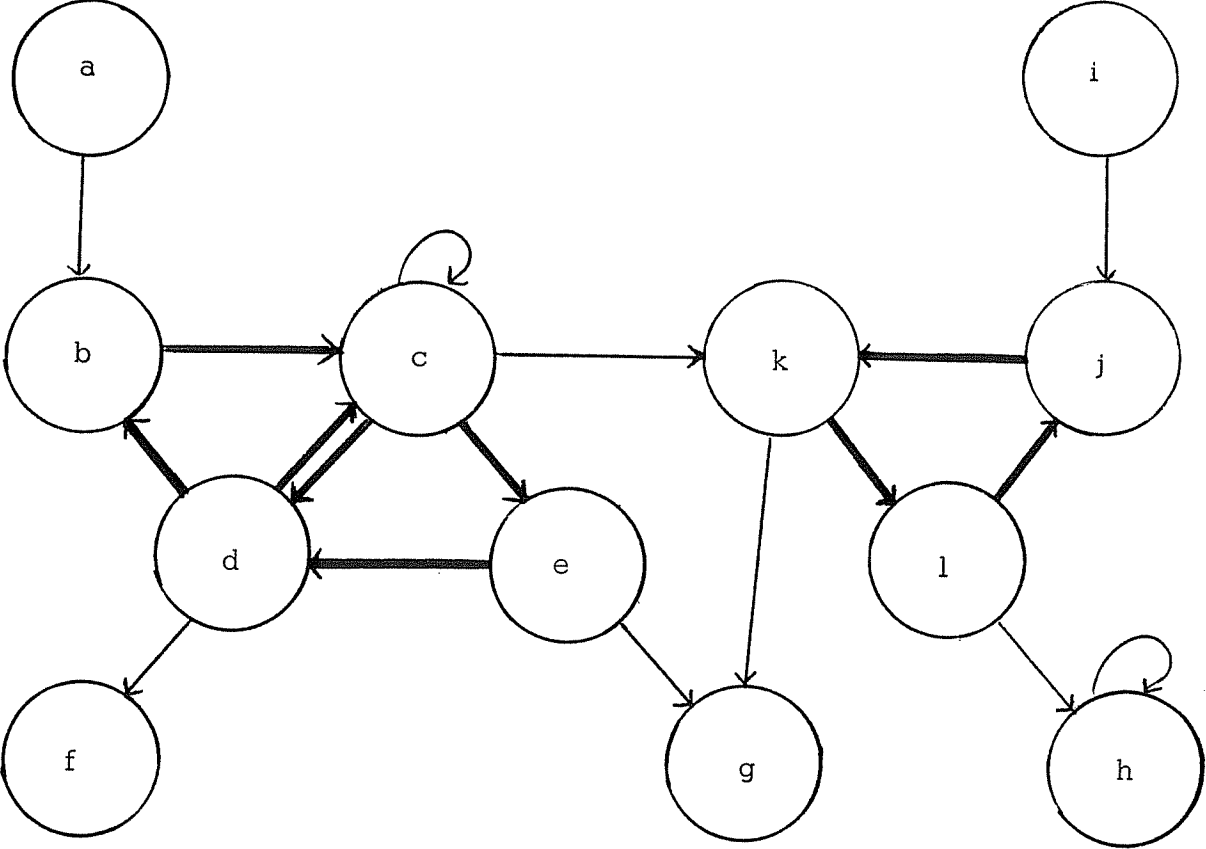
\includegraphics[width=.49\linewidth]{../img/purdom_g1.png}
    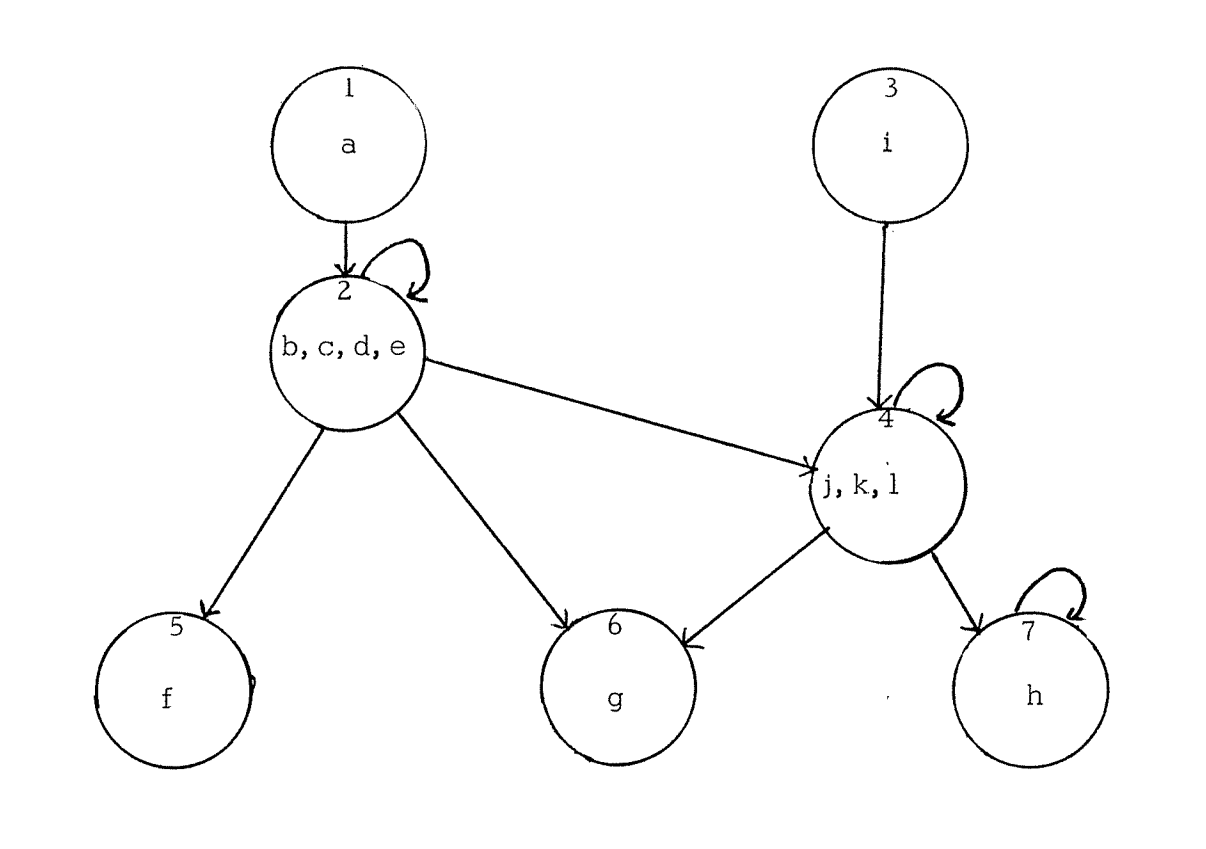
\includegraphics[width=.49\linewidth]{../img/purdom_g2b.png}
    \caption{aus \cite[Seite 78]{purdom1970transitive}}
\end{figure}

\begin{minipage}[t]{.5\textwidth}
test1
\end{minipage}
\begin{minipage}[t]{.5\textwidth}
test2
\end{minipage}

%\end{comment}

%% algo

\section{Vergleich der Suchalgorithmen}

Wie bereits erwähnt erfolgt die horizontale Suche pro Kode über alle Versionen ohne Vorkenntnisse vorheriger Suchergebnisse. Im Gegensatz dazu verarbeitet die vertikale Suche pro Version alle Kodes nur einmal, ist also allein deshalb schon effizienter, wenn Umsteiger für mehr als einen Kode ermittelt werden sollen. 

Wenn die Daten zusätlich aus einer Datenbank gelesen werden, ist die Anzahl an Aufrufen der readData-Funktion wesentlich entscheidender als die Menge an Ergebnissen pro Aufruf. Denn das Verbinden mit der Datenbank und Auslösen eines Suchbefehls dauert eine gewisse Zeit, was sich bei sehr vielen Aufrufen schnell aufaddiert. Dementsprechend ist es wesentlich schneller, alle Umsteiger einer Version auf einmal zu lesen, statt einzeln. 

Andererseits würde wiederum das Abfragen zusätzlicher Informationen, wie beispielsweise der Titel der Kodes eines Umsteigers vorher und nachher, bei der vertikalen Suche schnell die Größe der Daten im Arbeitsspeicher ansteigen lassen, weil pro Aufruf immer alle Umsteiger pro Version zwischengespeichert werden. 

Daher werden die beiden Algorithmen für unterschiedliche Zwecke eingesetzt.

Horizontale Suche:

\begin{itemize}
\item Darstellung der Umsteiger eines einzelnen Kodes mit Zusatzinformationen
\end{itemize}

Vertikale Suche: 

\begin{itemize}
\item Schreiben einer ConceptMap
\item Für alle Kodes einer Version bestimmen, ob diese Umsteiger haben (ja/nein)
\end{itemize}

\section{Schreiben der FHIR ConceptMap}

Dieser Abschnitt bezieht sich auf die in Kapitel \ref{conceptmap-structure} beschriebene ConceptMap-Struktur. 

Die anonyme Funktion, die der vertikalen Suche übergeben werden kann, dient zum Schreiben der ConceptMap. Jeder Aufruf der Funktion innerhalb des Algorithmus verfügt über die Daten, die zum Schreiben einer \emph{group} an Umsteigern mit Start- und Zielversion benötigt werden. Ein Durchlauf der vertikalen Suche kann dann mehrere Gruppen generieren, die ein Mapping auf eine Zielversionen ausgehend von allen anderen Versionen des Kodiersystems ermöglichen. Ebenfalls kann die Kombination mehrerer vertikalen Suche für jede Version als Zielversion aufgerufen werden, um so eine ConceptMap von allen Versionen auf alle Versionen zu schreiben.

Eine alle Versionen umfassende ConceptMap wird jedoch sehr groß. Zum Beispiel für die ICD-10-GM mit allen Kodes aus allen Versionen im XML-Format ist die Datei circa 1 GB groß. Wie in \cite{braaksma2014streaming} beschrieben macht es Sinn solche Dateien zu streamen, denn andernfalls müsste die komplette Datei im Arbeitsspeicher des Servers geschrieben werden. Die Vorgehensweise über die anonymen Funktionen ermöglicht genau das Streaming, weil nach jedem Aufruf der Ausgabepuffer des Servers geleert werden kann. Ein weiterer Vorteil ist, dass selbst wenn ein User sehr große ConceptMaps generieren lässt, der Download-Fortschritt über das Streaming angezeigt wird.  

Konkret enthält jede Iteration der anonymen Funktion die Informationen über Zielversion, aktuelle verarbeitete Version, sowie die vereinigten Umsteiger über alle vorher verarbeiteten Versionen. Zusätzlich muss allerdings noch bekannt sein, welche Kodes insgesamt in der Startversion vorhanden sind; zum einen, um Kodes ohne Umsteiger abzudecken und zum anderen, um keine Umsteiger aus vorher verarbeiteten Version aufzunehmen, deren Ursprungskode in der aktuellen Version nicht existiert. Hierfür ist also ein weiterer readData-Aufruf notwendig. Aus dem Vergleich dieser Kodes mit den Einträgen in der Merge-Datenstruktur können die Relationen für das Mapping bestimmt werden:

{
\renewcommand{\arraystretch}{1.2}
%\setlength{\tabcolsep}{12pt}
\begin{tabular}{ll}
%\uzlemph{Kode} & \uzlemph{Titel} \\
Kode in Merge-Daten enthalten? & Relation (R4) \\
\hline
Nein & \emph{equivalent} \\
Ja, übergeleitet auf UNDEF & \emph{unmatched} \\
Ja, übergeleitet auf einen Kode & \emph{related-to} \\
Ja, überleitetet auf mehrere Kodes & \emph{wider} \\
\end{tabular}
}

%, weil wie in (§Verweis) beschrieben die Liste der vereinigten Umsteiger immer auch Einträge aus vorher verarbeiteten Versionen enthalten durch die rückwärts topologische Vorgehensweise bedingt. Also zum Beispiel Kodes die in neueren Versionen erst hinzukommen. Außerdem wird über die beiden Informationen Umsteiger über die Versionen zwischen Start und Ziel sowie Kodes der Startversion die relationship bestimmt.

%Kode in Startversion;  Kode in Vereinigte Umsteiger; relationship
%vorhanden; Liste an Umsteigern; wider
%vorhanden; ein Umsteiger; related-to
%vorhanden; => UNDEF; unmapped
%vorhanden; nicht vorhanden; equivalent

Ablauf des Schreibens einer ConceptMap mit einer einzelnen Zielversion: 

\begin{enumerate}
\item Anfang der ConceptMap schreiben: \emph{ConceptMap}, \emph{url}, \emph{id}.
\item Vertikale Suche mit anonymer Funktion starten; jeder Aufruf generiert eine \emph{group}. \newline
Für jeden Kode wird ein \emph{element$\rightarrow$code}, \emph{element$\rightarrow$target$\rightarrow$code} Paar geschrieben -- \newline oder bei Relation \emph{wider} entsprechend mehrere \emph{target$\rightarrow$code} Einträge. 
\item Ende der ConceptMap schreiben.
\end{enumerate}

%Außerdem erlaubt die Vorgehensweise mit der anonymen Funktion ein Streaming der Datei. Das heißt muss nicht erst komplett im Arbeitsspeicher erstellt werden. Selbst wenn Umsteiger von allen Versionen als Start auf alle Versionen als Ziel geschrieben werden soll, werden als Daten im Arbeitsspeicher nur maximal die Sammlung der vereinigten Umsteiger von Start zu Ziel (oder andersherum) 

Eine Beispiel-ConceptMap im XML-Format befindet sich im Appendix \ref{conceptmap-example}.

